%==============================================================================
%  ĐỒ ÁN TỐT NGHIỆP — Nhận Dạng Từ Khóa Ít Mẫu Tập Mở ở Quy Mô Từ Vựng Lớn
%  Bản dịch tiếng Việt của thesis_en_2026.tex
%  Overleaf-ready (compiler: pdfLaTeX).
%
%  Thư mục hình ảnh: ./assets/ — tải cả thư mục này lên Overleaf cùng file .tex.
%
%  ---------------------------------------------------------------------------
%  QUY ƯỚC ĐÁNH DẤU (để phân biệt nội dung gốc và nội dung thêm mới):
%    \NEW{...}       -> văn bản thêm vào trong mục ĐÃ CÓ — màu xanh + ký hiệu [+]
%    \reviewnote{...}-> banner vàng — MỤC/PHẦN HOÀN TOÀN MỚI
%    \colabfig{...}  -> hộp đỏ — hình cần xuất từ Colab
%==============================================================================
\documentclass[12pt,a4paper]{report}

\usepackage[utf8]{inputenc}
\usepackage[T5]{fontenc}
\usepackage[vietnamese]{babel}
\usepackage{lmodern}
\usepackage{microtype}
\usepackage[a4paper,margin=2.5cm]{geometry}

\usepackage{amsmath,amssymb,amsfonts}
\usepackage{graphicx}
\graphicspath{{assets/}}
\usepackage{booktabs}
\usepackage{multirow}
\usepackage{array}
\usepackage[table,dvipsnames]{xcolor}
\usepackage{caption}
\usepackage{subcaption}
\usepackage{enumitem}
\usepackage{tikz}
\usepackage{pgfplots}
\pgfplotsset{compat=1.18}
\usetikzlibrary{arrows.meta,positioning,fit,backgrounds,calc}
\usepackage{algorithm}
\usepackage{algpseudocode}
\usepackage{setspace}
\onehalfspacing
\usepackage[hidelinks,colorlinks=true,linkcolor=blue!55!black,
            citecolor=blue!55!black,urlcolor=blue!55!black]{hyperref}
\usepackage{cleveref}
\usepackage{float}

\captionsetup{font=small,labelfont=bf}

%------------------------------ ký hiệu đánh dấu ----------------------------
% CÔNG TẮC DUYỆT: đặt \reviewmarkstrue để HIỆN đánh dấu (tự rà soát nội dung
% thêm mới), đặt \reviewmarksfalse để có BẢN SẠCH gửi hội đồng (ẩn banner vàng
% và bỏ tô màu chữ thêm). Hộp \colabfig luôn hiển thị vì là việc còn tồn đọng.
\newif\ifreviewmarks
\reviewmarksfalse
\definecolor{addcolor}{rgb}{0.05,0.25,0.6}
\ifreviewmarks
  \newcommand{\NEW}[1]{{\color{addcolor}#1\,\textsuperscript{\tiny[+]}}}
  \newcommand{\reviewnote}[1]{%
    \par\smallskip\noindent
    \colorbox{yellow!35}{\parbox{0.97\linewidth}{\small\textbf{[XEM XÉT — MỤC MỚI DO TRỢ LÝ VIẾT]}\; #1}}%
    \par\smallskip}
\else
  \newcommand{\NEW}[1]{#1}
  \newcommand{\reviewnote}[1]{}
\fi
\newcommand{\colabfig}[1]{%
  \par\smallskip\begin{center}
  \fcolorbox{red!60!black}{red!6}{\parbox{0.9\linewidth}{\centering\small
  \textbf{[HÌNH CẦN XUẤT TỪ COLAB]}\\[2pt] #1}}\end{center}\par\smallskip}

\newcommand{\code}[1]{\texttt{\small #1}}
\newcommand{\acc}{\text{ACC}}
\newcommand{\far}{\text{FAR}}
\newcommand{\frr}{\text{FRR}}
\newcommand{\eer}{\text{EER}}
\newcommand{\auc}{\text{AUC}}
\newcommand{\R}{\mathbb{R}}
\newcommand{\norm}[1]{\lVert #1\rVert}
\newcommand{\best}[1]{\textbf{#1}}

%==============================================================================
\begin{document}

%------------------------------ trang bìa ------------------------------------
\begin{titlepage}
\thispagestyle{empty}
\begin{tikzpicture}[remember picture, overlay]
  \draw[line width=0.8pt]
    ([shift={(1.6cm,1.6cm)}]current page.south west)
    rectangle
    ([shift={(-1.6cm,-1.6cm)}]current page.north east);
\end{tikzpicture}%
\centering
\vspace*{0.6cm}
{\normalsize\bfseries TRƯỜNG ĐẠI HỌC KHOA HỌC VÀ CÔNG NGHỆ HÀ NỘI\par}
{\normalsize\bfseries KHOA CÔNG NGHỆ THÔNG TIN VÀ TRUYỀN THÔNG\par}
\vspace{1.3cm}

\includegraphics[width=4.5cm]{Logo_USTH.png}\par
\vspace{1.1cm}
{\Huge\bfseries ĐỒ ÁN TỐT NGHIỆP\par}
\vspace{0.7cm}
{\large Sinh viên thực hiện\par}
{\large\bfseries Phạm Hoàng An - 23BI14002\par}
\vspace{1.0cm}
{\large\bfseries Đề tài:\par}
{\large Nhận Dạng Từ Khóa Ít Mẫu Tập Mở ở Quy Mô Từ Vựng Lớn\par}
\vspace{0.25cm}
{\normalsize Nghiên Cứu Học Độ Đo về Bộ Trích Xuất Đặc Trưng, Bộ Mã Hóa\\
và Phương Pháp Từ Chối Tập Mở\par}
\vfill
{\large Giảng viên hướng dẫn:\quad TS.\ Trần Hoàng Tùng\par}
\vspace{1.6cm}
{\large\bfseries Hà Nội, tháng 6 năm 2026\par}
\vspace*{0.5cm}
\end{titlepage}

%------------------------------ trang xác nhận -------------------------------
\thispagestyle{empty}
\vspace*{2.5cm}
\begin{center}
Kính gửi các bên liên quan,
\end{center}
\vspace{0.6cm}
\noindent Tôi, TS.\ Trần Hoàng Tùng, xác nhận rằng đồ án / báo cáo thực tập của
Ông Phạm Hoàng An đủ điều kiện để trình bày trước Hội đồng Thực tập
2025--2026.
\vspace{2.5cm}
\begin{flushright}
Hà Nội, tháng 6 năm 2026\\[1.4cm]
\textbf{Chữ ký của giảng viên hướng dẫn}
\end{flushright}
\clearpage

% Phần đầu (bìa/cảm ơn/tóm tắt/mục lục) đánh số La Mã; Chương 1 sẽ đặt lại số Ả Rập.
\pagenumbering{roman}

%------------------------------ lời cảm ơn -----------------------------------
\chapter*{Lời Cảm Ơn}
\addcontentsline{toc}{chapter}{Lời Cảm Ơn}

Trước hết, em xin bày tỏ lòng biết ơn sâu sắc tới giảng viên hướng dẫn,
TS.\ Trần Hoàng Tùng, vì những phản hồi sâu sắc và sự hướng dẫn tận tình trong
suốt 3 tháng thực tập. Em cũng xin chân thành cảm ơn TS.\ Trần Giang Sơn đã tạo
điều kiện cho em toàn quyền sử dụng máy chủ ICTLab, giúp phần tính toán của đồ
án thành công tốt đẹp.

Xin cảm ơn gia đình đã luôn động viên và ủng hộ về mặt tinh thần, giúp em duy
trì động lực và hoàn thành đồ án này. Em cũng xin gửi lời cảm ơn tới những ai đã
dành thời gian đọc và góp ý cho đồ án.

%------------------------------ tóm tắt -------------------------------------
\chapter*{Tóm Tắt}
\addcontentsline{toc}{chapter}{Tóm Tắt}

Chúng tôi nghiên cứu bài toán \emph{nhận dạng từ khóa ít mẫu tập mở} (Few-Shot
Open-Set Keyword Spotting --- KWS): một bộ mã hóa embedding duy nhất được huấn
luyện một lần trên kho từ vựng lớn, sau đó được triển khai để nhận dạng tập từ
khóa tùy chọn của người dùng từ chỉ một số ít mẫu đăng ký, đồng thời từ chối
lời nói ngoài từ điển và tiếng im lặng. Chúng tôi xây dựng một pipeline hoàn
toàn tái tạo được xoay quanh hai bộ mã hóa nhỏ gọn --- mạng tích chập phân tách
theo chiều sâu DSCNN-L ($\approx$0{,}41\,M tham số) và mô hình cạnh chú ý thời gian
EdgeSpot-Full $\tau{=}4$ ($\approx$0{,}13\,M tham số) --- kết hợp với ba bộ trích
xuất đặc trưng (MFCC, log-mel và PCEN theo kênh có thể học được) và bốn hàm mục
tiêu học độ đo (Triplet, Sub-center ArcFace (SCAF), Generalized End-to-End (GE2E)
và Knowledge Distillation cosine (KD) từ mô hình giáo viên Wav2Vec\,2.0 đã đóng
băng). Toàn bộ hệ thống được huấn luyện trên Multilingual Spoken Words Corpus
(MSWC) tiếng Anh và đánh giá chéo kho ngữ liệu trên Google Speech Commands v2
(GSC) theo giao thức EdgeSpot-exact 10 mẫu tập mở với 100 lần chạy ngẫu nhiên.
Qua bộ sàng lọc 16 cấu hình chúng tôi chỉ ra rằng:
(i) bộ trích xuất PCEN có thể học được là cải tiến đáng tin cậy nhất (lên tới
$+9{,}2$ điểm độ chính xác tại tỷ lệ chấp nhận sai 1\% cho bộ mã hóa cạnh);
(ii) hàm mục tiêu GE2E dựa trên centroid vượt trội so với các hàm mục tiêu phân
loại trong tổng quát hóa tập mở;
(iii) quan trọng nhất, hàm mục tiêu phân loại SCAF sụp đổ khi từ vựng huấn luyện
tăng lên $37{.}387$ lớp nếu trọng số loss không được giảm bốn bậc độ lớn.
Chúng tôi thêm vào đó đặc trưng hóa việc độ chính xác bão hòa gần hai triệu
clip huấn luyện và chứng minh rằng hàm mục tiêu KD cosine đạt độ chính xác ngang
GE2E với khoảng một nửa dữ liệu. Cấu hình tốt nhất tổng thể (DSCNN-L + PCEN +
GE2E) đạt $86{,}36\%$ độ chính xác tập mở tại 1\% FAR và AUC $95{,}21$ trên GSC
test, trong khi mô hình nhỏ gọn nhất (EdgeSpot-Full + PCEN + GE2E) đạt $82{,}87\%$
với một phần ba số tham số. Chúng tôi công bố mã nguồn đầy đủ, các giao thức
huấn luyện/đánh giá và bản demo web chạy offline.

\bigskip
\noindent\textbf{Từ khóa:} nhận dạng từ khóa, học ít mẫu, nhận dạng tập mở, học
độ đo, PCEN, GE2E, MSWC, Google Speech Commands.

%------------------------------ mục lục --------------------------------------
\tableofcontents

%==============================================================================
% Đặt lại số trang Ả Rập, bắt đầu từ Chương 1.
\clearpage
\pagenumbering{arabic}
\chapter{Giới Thiệu}\label{ch:intro}

Chương này giới thiệu bài toán mà đồ án giải quyết và lý do nó quan trọng. Mục
\Cref{sec:context} đặt nhận dạng từ khóa vào bối cảnh các giao diện thoại hiện đại
và nêu động lực chuyển từ thiết kế tập đóng sang tập mở ít mẫu. \Cref{sec:objectives}
phát biểu các mục tiêu của đồ án và \Cref{sec:outcomes} nêu các kết quả kỳ vọng.
\Cref{sec:plain} giải thích bài toán theo ngôn ngữ thông thường. Cuối cùng,
\Cref{sec:thesisstruct} trình bày cấu trúc của toàn bộ đồ án.

Trước khi đi vào chi tiết, \Cref{fig:overview} tóm tắt toàn cảnh hệ thống ở mức
khái niệm: bộ mã hóa được \emph{huấn luyện một lần} để học cách so sánh hai âm thanh; khi triển khai, người dùng \emph{đăng ký} vài mẫu
cho mỗi từ khóa để tạo các điểm đại diện (prototype); mỗi âm thanh đến được
\emph{khớp} với prototype gần nhất; và nếu nó nằm xa mọi prototype thì bị
\emph{từ chối} là ``không phải từ khóa''. Toàn bộ đồ án xoay quanh bốn bước này.

\begin{figure}[H]
\centering
\resizebox{\linewidth}{!}{%
\begin{tikzpicture}[
  node distance=6mm and 9mm,
  stage/.style={draw,rounded corners=3pt,align=center,minimum height=11mm,
              minimum width=24mm,font=\footnotesize,fill=blue!5},
  arr/.style={-{Latex[length=2.4mm]},thick},
  lbl/.style={font=\scriptsize\itshape,align=center,text=black!60}]
\node[stage] (train) {\textbf{1. Huấn luyện một lần}\\học so sánh âm thanh\\(kho từ vựng lớn)};
\node[stage,right=of train] (enroll) {\textbf{2. Đăng ký}\\vài mẫu mỗi từ khóa\\$\to$ prototype};
\node[stage,right=of enroll] (match) {\textbf{3. Khớp}\\prototype gần nhất\\trong không gian embedding};
\node[stage,right=of match] (reject) {\textbf{4. Quyết định}\\từ khóa \emph{hoặc}\\``không biết''};
\draw[arr](train)--(enroll);
\draw[arr](enroll)--(match);
\draw[arr](match)--(reject);
\node[lbl,below=3mm of train]{mô hình cố định\\sau bước này};
\node[lbl,below=3mm of enroll]{người dùng tự\\định nghĩa từ khóa};
\node[lbl,below=3mm of reject]{từ chối tập mở};
\end{tikzpicture}}
\caption{Toàn cảnh hệ thống nhận dạng từ khóa ít mẫu tập mở ở mức khái niệm: huấn
luyện một lần $\to$ đăng ký $\to$ khớp prototype gần nhất $\to$ quyết định tập mở.
Sơ đồ kỹ thuật chi tiết được trình bày ở \Cref{fig:pipeline}.}
\label{fig:overview}
\end{figure}

\section{Bối Cảnh và Động Lực}\label{sec:context}

Nhận dạng từ khóa (Keyword Spotting --- KWS) --- bài toán phát hiện một tập lệnh
thoại nhỏ trong luồng âm thanh liên tục --- là cổng vào luôn bật của hầu hết mọi
giao diện thoại hiện đại. Các hệ thống KWS cổ điển được huấn luyện dưới dạng bộ
phân loại tập đóng trên một từ điển cố định (ví dụ mười từ lệnh của Google Speech
Commands). Thiết kế này có hai hạn chế cấu trúc. Thứ nhất, tập từ khóa bị đóng
băng tại thời điểm huấn luyện: hỗ trợ một từ đánh thức hoặc lệnh mới đòi hỏi
phải thu thập dữ liệu và huấn luyện lại mô hình. Thứ hai, bộ phân loại softmax
về bản chất không phải là tập mở: mọi đầu vào đều bị ép vào một trong các lớp đã
biết, nên từ chưa từng gặp và tiếng ồn nền bị nhầm thành lệnh, gây ra kích hoạt
nhầm. Công trình này hướng đến bài toán ít mẫu tập mở thực tế hơn và khó hơn. Chúng tôi huấn luyện một bộ mã hóa embedding duy nhất
trên kho từ vựng rất lớn và đa dạng; khi triển khai, người dùng cuối tự định
nghĩa tập từ khóa bằng cách cung cấp chỉ vài ($k$) mẫu đăng ký cho mỗi
từ. Mỗi từ khóa được đại diện bởi một \emph{prototype} (trung bình embedding của
các mẫu đăng ký); nhận dạng được thực hiện bằng cách khớp prototype gần nhất
trong không gian embedding, và một quyết định tập mở tường minh từ chối bất kỳ
âm thanh nào quá xa tất cả các prototype. Vấn đề chúng tôi theo đuổi xuyên suốt
đồ án là điều gì khiến một bộ mã hóa như vậy tổng quát hóa được, và cần xử lý
bài toán ở quy mô từ vựng huấn luyện nào --- một từ vựng nhỏ liệu
có đủ hay bắt buộc phải lớn, và nếu lớn thì lớn đến mức nào --- để đạt được khả
năng tổng quát hóa đó.

\paragraph{Đóng góp.} Các đóng góp chính gồm:
\begin{itemize}[leftmargin=1.4em,itemsep=2pt]
\item Một framework KWS ít mẫu tập mở dễ tái tạo, ít phụ thuộc, với hai bộ mã
hóa nhỏ gọn, ba bộ trích xuất đặc trưng, bốn hàm mục tiêu độ đo và bốn đầu từ
chối tập mở, tất cả chia sẻ giao diện prototype chung (\Cref{ch:method}).
\item Bộ sàng lọc 16 cấu hình trên MSWC toàn từ vựng, cô lập đóng góp từng trục
bằng các delta cặp; PCEN và GE2E nổi lên là hai lợi thế ổn định
(\Cref{ch:results}).
\item Phân tích quy mô cho thấy:
\begin{itemize}[leftmargin=1.3em,itemsep=1pt]
\item Độ chính xác bão hòa gần $\sim$2\,M clip huấn luyện; và
\item Chế độ thất bại của Sub-center ArcFace tại $37$k lớp, kèm giải thích theo
cơ chế gradient và cách khắc phục thực tế (\Cref{ch:results}).
\end{itemize}
\item Nghiên cứu knowledge distillation cho thấy hàm mục tiêu cosine với mô hình
giáo viên Wav2Vec\,2.0 đóng băng đạt độ chính xác ngang GE2E với khoảng một nửa
dữ liệu huấn luyện (\Cref{ch:results}).
\item Đánh giá chéo kho ngữ liệu hoàn chỉnh theo giao thức EdgeSpot-exact 10
mẫu (100 lần chạy), kèm pipeline phát trực tuyến trên CPU (Silero VAD + máy
trạng thái làm mượt) và bản demo web chạy offline (\Cref{ch:method}).
\end{itemize}

%------------------------------------------------------- MỤC MỚI 1.3 ---------
\section{Mục Tiêu Đề Tài}\label{sec:objectives}
\reviewnote{Mục mới, mô phỏng theo mục ``Mục Tiêu Đề Tài'' của đồ án mẫu.}

Mục tiêu chính của đồ án là thiết kế, triển khai và đánh giá nghiêm ngặt một hệ
thống nhận dạng từ khóa tập mở \emph{không cần huấn luyện lại}, học một embedding
có thể chuyển giao duy nhất và hỗ trợ từ điển tùy chọn của người dùng từ một số
ít mẫu đăng ký. Cụ thể, chúng tôi hướng đến:
\begin{enumerate}[leftmargin=1.5em,itemsep=2pt]
\item Xây dựng bộ mã hóa nhỏ gọn, hoạt động offline trên phần cứng bình thường;
\item Xác định, qua nghiên cứu nhân tố có kiểm soát, bộ trích xuất đặc trưng, cấu
trúc bộ mã hóa và hàm mục tiêu độ đo nào tổng quát hóa tốt nhất giữa các kho ngữ
liệu;
\item Đặc trưng hóa hành vi của các lựa chọn thiết kế khi từ vựng huấn luyện tăng
từ vài chục đến vài chục nghìn từ; và
\item Cung cấp đánh giá tập mở trung thực (DET/AUC/EER/ACC@FAR) theo giao thức
nghiêm ngặt, có thể tái tạo, kèm bản demo phát trực tuyến hoạt động được.
\end{enumerate}

\section{Kết Quả Kỳ Vọng}\label{sec:outcomes}
\reviewnote{Mục mới, mô phỏng theo mục ``Kết Quả Kỳ Vọng'' của đồ án mẫu.}

Hệ thống được kỳ vọng: (i) nhận dạng tập từ khóa do người dùng tự tạo được đăng
ký từ $\le 10$ mẫu mỗi từ mà không cần huấn luyện lại; (ii) từ chối lời nói ngoài
từ điển và tiếng im lặng với tỷ lệ chấp nhận sai có thể kiểm soát được; (iii) tổng
quát hóa qua các điều kiện ghi âm, chứng minh bằng cách huấn luyện trên một kho
ngữ liệu (MSWC) và kiểm tra trên một kho ngữ liệu hoàn toàn khác (GSC); và (iv) đủ
nhỏ để triển khai offline trên thiết bị đầu cuối. Các sản phẩm đi kèm gồm các bộ
mã hóa đã huấn luyện, các script huấn luyện/đánh giá và bản demo web offline có
phân tích thời điểm từ khóa trên audio dài.

%------------------------------------------------------------------ MỤC MỚI 1.4
\section{Giải Thích Bài Toán Theo Ngôn Ngữ Thông Thường}\label{sec:plain}
\reviewnote{Mục mới --- giải thích bài toán cho người đọc không chuyên, giọng văn
khách quan, độ dài khoảng một trang.}

Nhận dạng từ khóa là thành phần phần mềm luôn chạy nền của các thiết bị điều khiển
bằng giọng nói (loa thông minh, tai nghe), có nhiệm vụ phát hiện một số lệnh
thoại ngắn như ``dừng lại'', ``tiếp theo'' hoặc một từ đánh thức. Do phải hoạt
động liên tục, nó được thiết kế nhỏ và tiết kiệm năng lượng; bộ nhận dạng giọng nói đầy đủ, vốn tốn tài nguyên, chỉ được kích hoạt
\emph{sau khi} từ khóa đã được phát hiện. Vì vậy, nhận dạng từ khóa đóng vai trò
cổng vào của hầu hết các giao diện thoại.

\paragraph{Hạn chế của cách tiếp cận tập đóng.}
Phần lớn hệ thống nhận dạng từ khóa thương mại được huấn luyện dưới dạng bộ phân
loại trên một danh sách từ \emph{cố định} (ví dụ mười lệnh \textit{yes, no, up,
down, \dots}).
Thiết kế này có hai hạn chế. Thứ nhất, tập từ khóa bị cố định tại thời
điểm huấn luyện: muốn thêm một lệnh hoặc từ mới, nhà sản xuất phải thu
thập dữ liệu và huấn luyện lại mô hình. Thứ hai, một bộ phân loại tập đóng buộc
phải chọn một nhãn cho \emph{mọi} đầu vào, kể cả tiếng ho, tiếng nhạc hay một từ
chưa từng gặp; hệ quả là thiết bị bị \emph{kích hoạt nhầm} khi không có lệnh nào
thực sự được nói ra.

\paragraph{Hướng tiếp cận của đồ án.}
Đồ án xây dựng hệ thống theo hướng \emph{học độ đo}: thay vì ghi nhớ một danh sách
nhãn cố định, mô hình học một kỹ năng tổng quát hơn là xác định hai đoạn âm thanh
có cùng một từ hay không. Kỹ năng này được huấn luyện một lần trên một kho từ
nói lớn và đa dạng. Khi triển khai, người dùng tự định nghĩa tập lệnh
bằng cách cung cấp một vài mẫu ghi âm cho mỗi từ, và hệ thống không cần huấn luyện
lại. Về mặt biểu diễn, mỗi lệnh được tóm lược thành một điểm đại diện trong một
không gian đặc trưng (\emph{embedding}); để nhận dạng, hệ thống ánh xạ âm thanh
mới vào không gian này và xét xem nó gần điểm đại diện của lệnh nào nhất. Nếu âm
thanh nằm xa tất cả các lệnh đã đăng ký, hệ thống đưa ra kết luận ``không phải từ
khóa'' --- đây chính là năng lực \emph{tập mở}, cho phép bỏ qua lời nói không liên
quan và tiếng ồn.

\paragraph{Ý nghĩa thực tiễn và thách thức.}
Cách tiếp cận này mang lại ba lợi ích: (i) cá nhân hóa mà không cần huấn luyện lại,
phù hợp với trợ lý chạy trên thiết bị, công cụ hỗ trợ tiếp cận và điều khiển công
nghiệp tùy biến; (ii) giảm kích hoạt nhầm nhờ khả năng từ chối; và (iii) kích
thước mô hình nhỏ ($\sim$0{,}1--0{,}4 triệu tham số), đủ để chạy offline trên thiết
bị, bảo vệ quyền riêng tư. Đồng thời, bài toán đặt ra ba thách thức chính. Thứ
nhất là \emph{tổng quát hóa}: mô hình phải hoạt động trên các từ, thiết bị ghi âm
và giọng nói chưa gặp khi huấn luyện, nên đồ án cố tình huấn luyện trên một kho
ngữ liệu và đánh giá trên một kho khác. Thứ hai là \emph{ranh giới tập
mở}: việc từ chối đáng tin cậy không gian rất lớn của ``mọi thứ không phải lệnh''
khó hơn nhiều so với một vài lệnh đã biết, và cần định lượng trung thực
đánh đổi giữa từ chối quá mức và từ chối quá yếu. Thứ ba là \emph{quy mô}: khi từ
vựng huấn luyện tăng từ vài chục lên gần bốn mươi nghìn từ, một số kỹ thuật vốn
hiệu quả ở quy mô nhỏ lại thất bại --- một hiện tượng được phân tích ở
\Cref{ch:results}.

\section{Cấu Trúc Đồ Án}\label{sec:thesisstruct}
\reviewnote{Mục mới --- giới thiệu bố cục các chương, theo chuẩn đồ án.}

Phần còn lại của đồ án được tổ chức như sau. \Cref{ch:background} trình bày kiến
thức nền tảng: cách âm thanh được số hóa và biểu diễn dưới dạng mel-spectrogram,
sự khác biệt giữa nhận dạng tập đóng và tập mở, ý tưởng học ít mẫu và học độ đo,
cùng các công trình liên quan mà đồ án kế thừa. \Cref{ch:method} mô tả phương pháp
đề xuất: phát biểu bài toán, các bộ trích xuất đặc trưng, hai bộ mã hóa, các hàm
mục tiêu học độ đo, các đầu từ chối tập mở, phương pháp đánh giá và thiết kế thực
nghiệm --- chương này nêu \emph{những gì được làm và đo}.
\Cref{ch:results} trình bày và phân tích kết quả theo bốn câu hỏi nghiên cứu, gắn
với ý nghĩa sử dụng thực tế. \Cref{ch:conclusion} tổng kết hiện
trạng, điểm mạnh, điểm yếu và hướng phát triển tương lai.

%==============================================================================
\chapter{Kiến Thức Nền Tảng và Các Công Trình Liên Quan}\label{ch:background}
\reviewnote{Toàn bộ chương này là mới. Bao gồm kiến thức đại cương: âm thanh được
dùng như thế nào, dữ liệu có dạng ra sao, cách chuyển sang mel-spectrum, và các
công trình trước mà đồ án xây dựng trên đó.}

Chương này cung cấp kiến thức nền tảng cần thiết để hiểu phần phương pháp.
\Cref{sec:sound2data} mô tả cách âm thanh được số hóa thành dữ liệu mà máy tính
xử lý được; \Cref{sec:mel} trình bày biểu diễn thời gian--tần số (mel-spectrogram)
được dùng làm đầu vào cho mô hình. \Cref{sec:kws-bg} phân biệt nhận dạng từ khóa
tập đóng với tập mở, \Cref{sec:fewshot-bg} giới thiệu học ít mẫu và học độ đo, và
\Cref{sec:arc-bg} điểm qua các phương pháp biên góc cùng từ chối tập mở mà đồ án
kế thừa và so sánh.

\section{Từ Âm Thanh Đến Dữ Liệu Số}\label{sec:sound2data}

Âm thanh trong tự nhiên là một \emph{sóng áp suất liên tục} biến thiên theo thời
gian. Máy tính không lưu được tín hiệu liên tục, nên bước đầu tiên là \emph{số
hóa} qua hai thao tác: \emph{lấy mẫu} (sampling) đo biên độ sóng tại các thời
điểm cách đều nhau, và \emph{lượng tử hóa} (quantization) làm tròn mỗi giá trị đo
được về một số hữu hạn mức. Kết quả là một dãy số rời rạc đại diện cho dạng sóng.

Tần số lấy mẫu quyết định dải tần mà tín hiệu số còn giữ lại được. Theo
\emph{định lý lấy mẫu Nyquist}, một tần số lấy mẫu $f_s$ chỉ biểu diễn trung thực
các thành phần tần số dưới $f_s/2$. Năng lượng phân biệt các âm vị trong tiếng nói
tập trung dưới khoảng 8\,kHz, nên tần số $f_s = 16{.}000$ mẫu/giây (16\,kHz) ---
với giới hạn Nyquist 8\,kHz --- là đủ và đã trở thành tiêu chuẩn thực tế cho các
bài toán giọng nói. Tăng tần số lấy mẫu cao hơn chủ yếu làm tăng chi phí tính toán
mà ít cải thiện chất lượng nhận dạng từ. Toàn bộ đồ án dùng âm thanh 16\,kHz, một
kênh (mono).

Để mọi clip có cùng kích thước đầu vào, mỗi đoạn lệnh thoại được chuẩn hóa thành
đúng một giây, tương ứng một vector $16{.}000$ số (gọi là \emph{dạng sóng thô}):
clip ngắn hơn được đệm thêm các giá trị không ở hai đầu, clip dài hơn bị cắt bớt.
Việc cố định độ dài này giúp đóng gói dữ liệu thành batch và giữ cho bộ trích xuất
đặc trưng phía sau có kích thước tensor không đổi. \Cref{fig:audiofeat}(a) minh
họa một dạng sóng một giây của từ ``yes''.

\begin{figure}[H]
\centering
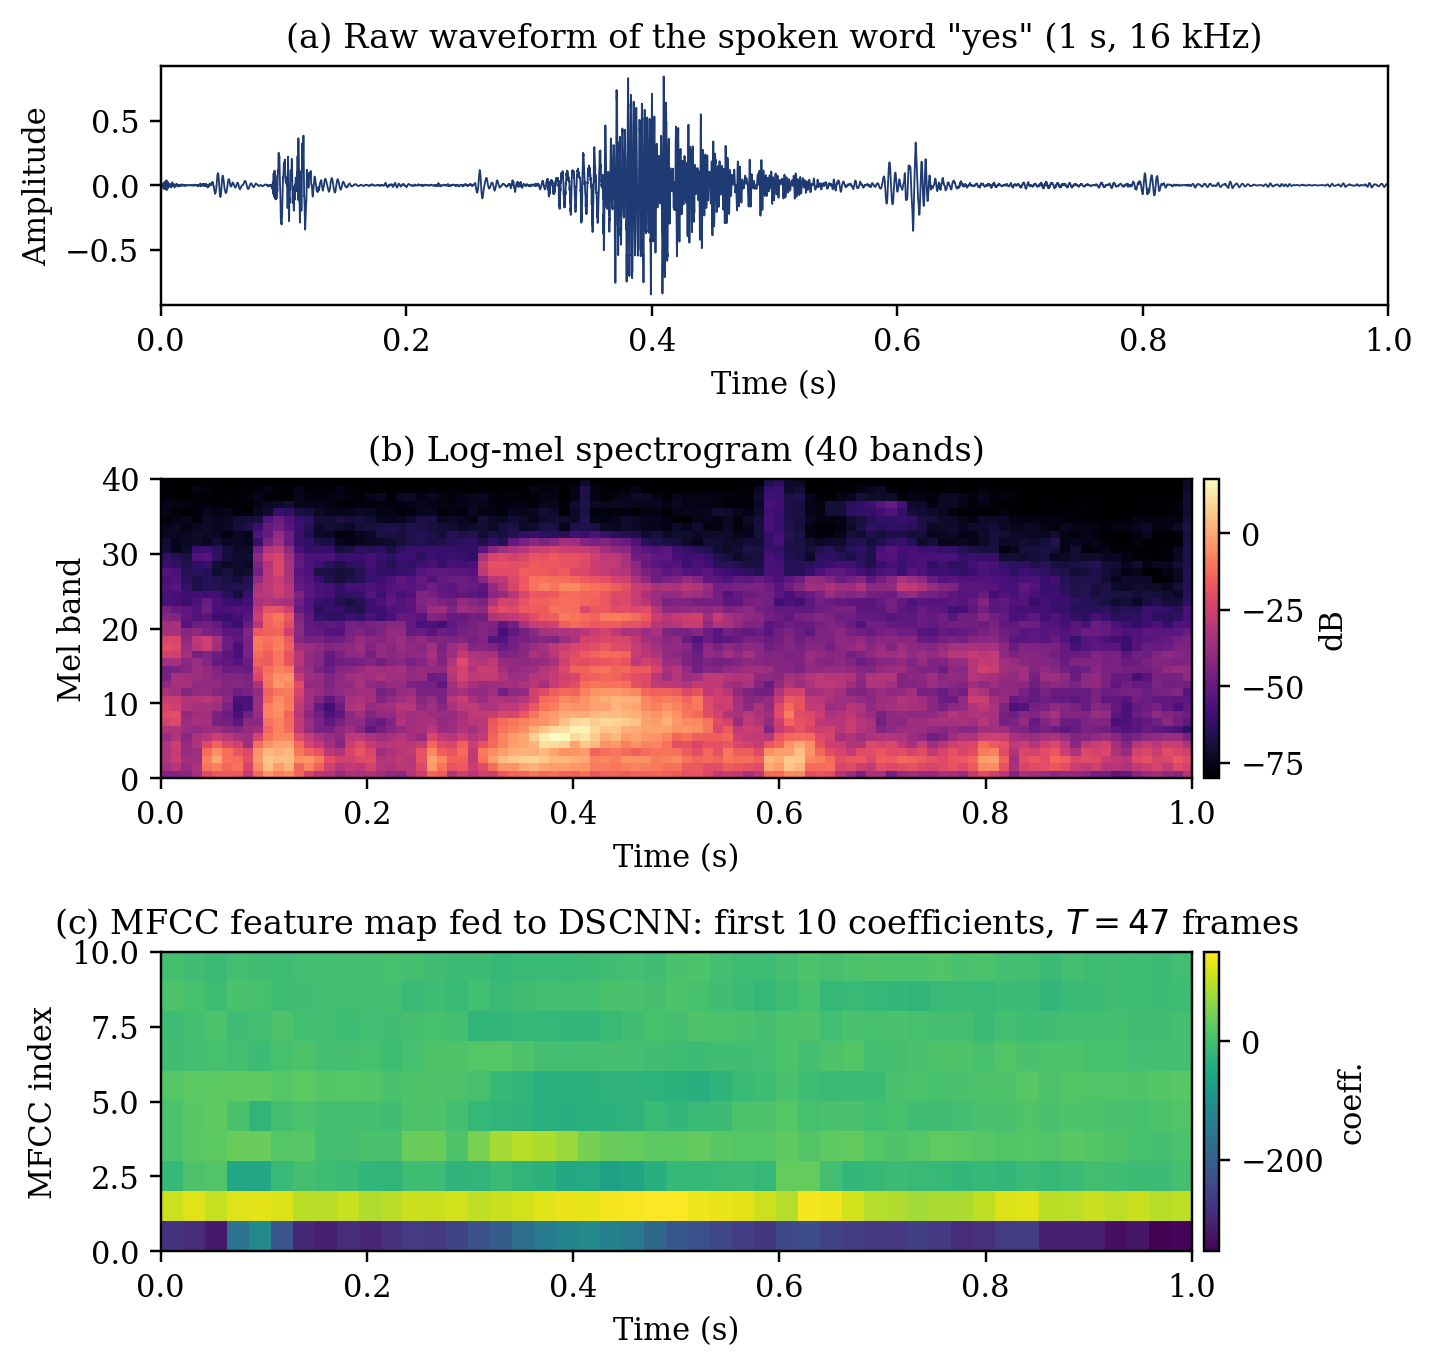
\includegraphics[width=0.92\linewidth]{fig_audio_features.png}
\caption{Từ âm thanh đến đặc trưng, tính từ bản ghi Google Speech Commands thật
của từ ``yes''.
(a) dạng sóng thô 1\,s, 16\,kHz;
(b) log-mel spectrogram 40 băng (ảnh thời gian--tần số tri giác);
(c) 10 hệ số MFCC đầu tiên trên $T{=}47$ khung --- tensor thực sự đưa vào bộ mã
hóa DSCNN.}
\label{fig:audiofeat}
\end{figure}

Tuy biểu diễn được tín hiệu, dạng sóng thô lại là đầu vào kém cho bộ phân loại.
Thứ nhất, nó có \emph{số chiều rất cao} ($16{.}000$ giá trị cho một giây). Thứ
hai, nó \emph{không bất biến với các biến đổi vô hại}: cùng một từ nói to hơn,
nói lệch thời gian một chút, hoặc thu ở thiết bị khác sẽ cho dãy mẫu rất khác nhau
ở mức từng điểm, dù tai người vẫn nghe ra cùng một từ. Vì vậy, thay vì đưa thẳng
dạng sóng vào mô hình, ta biến đổi nó sang một biểu diễn cô đọng và ổn định hơn
trong miền thời gian--tần số, trình bày ở \Cref{sec:mel}.

\section{Biểu Diễn Thời Gian--Tần Số: Mel-Spectrogram}\label{sec:mel}

Lời nói dễ mô hình hóa hơn nhiều trong miền \emph{thời gian--tần số}. Chúng tôi
trượt một cửa sổ phân tích ngắn (25--40\,ms) qua dạng sóng theo các bước nhảy nhỏ
(10--20\,ms) và, cho mỗi cửa sổ, tính biến đổi Fourier ngắn (STFT) để thu năng
lượng tại từng tần số. Hai thực tế tri giác về thính giác người hướng dẫn bước
tiếp theo: chúng ta cảm nhận độ cao âm thanh trên thang lôgarít, và nhạy cảm hơn
với sự khác biệt ở tần số thấp hơn ở tần số cao. \emph{Thang mel} mã hóa điều đó:
nó biến đổi tần số tuyến tính (Hz) thành trục mel tri giác theo công thức
\begin{equation}
m \;=\; 2595\,\log_{10}\!\Big(1+\frac{f}{700}\Big),
\label{eq:mel}
\end{equation}
trong đó $f$ là tần số tính bằng Hz và $m$ là giá trị tương ứng trên thang mel;
hằng số $700$ và $2595$ định hình đường cong sao cho ở vùng tần số thấp thang mel
gần tuyến tính với Hz, còn ở vùng tần số cao nó nén lại theo lôgarít --- phản ánh
đúng độ phân giải giảm dần của tai người. Nhờ vậy, một bộ (ở đây 40) bộ lọc tam
giác chồng lên nhau cách đều trên trục mel này tổng hợp năng lượng STFT vào 40
\emph{băng mel}, dành nhiều băng hơn cho vùng tần số mà tai người nhạy cảm. Lấy lôgarít của năng lượng băng
(vì độ to cũng được cảm nhận theo lôgarít) cho ra \emph{log-mel spectrogram} ở
\Cref{fig:audiofeat}(b): một ảnh nhỏ gọn trong đó trục ngang là thời gian, trục
dọc là tần số mel, và độ sáng là năng lượng.

\paragraph{MFCC.}
Một bước cổ điển nữa khử tương quan các băng log-mel bằng biến đổi cosin rời rạc
(DCT), tạo ra \emph{Hệ số Cepstral Tần Số Mel} (MFCC). Các hệ số bậc thấp nắm
bắt đường bao phổ biến đổi chậm (mang hầu hết thông tin âm vị), vì vậy thông
thường --- và chúng tôi làm theo --- chỉ giữ vài hệ số đầu tiên.
\Cref{fig:audiofeat}(c) cho thấy bản đồ 10 hệ số MFCC chúng tôi đưa vào bộ mã
hóa. Toàn bộ pipeline trích xuất đặc trưng vì vậy là một phép biến đổi cố định,
nhỏ, biến một giây âm thanh thành một ``ảnh'' một kênh có dạng
thời-gian$\times$đặc-trưng, mà mạng tích chập có thể xử lý.

\paragraph{PCEN.}
Lôgarít tĩnh dùng ở trên đơn giản nhưng không thích nghi với điều kiện ghi âm.
\emph{Chuẩn hóa Năng Lượng Theo Kênh} (Per-Channel Energy Normalization ---
PCEN)~\cite{wang2017trainable} thay thế bằng kiểm soát khuếch đại tự động theo
từng băng \emph{có thể học được} kèm nén mềm; các tham số của nó được học cùng với
mạng. PCEN được thiết kế cho phát hiện bền vững từ xa và, như \Cref{ch:results}
cho thấy, là cải tiến đáng tin cậy nhất trong nghiên cứu này. Phương trình chính
xác được trình bày tại \Cref{sec:frontends}.

\reviewnote{Hai hình minh họa dữ liệu mới bên dưới
(\ref{fig:dataexamples}, \ref{fig:melfb}), tạo từ dữ liệu dự án thật, theo phong
cách hình ảnh dữ liệu mẫu của đồ án ADAS tham khảo.}

Để xây dựng trực giác về những gì mô hình thực sự thấy, \Cref{fig:dataexamples}
cho thấy log-mel spectrogram của sáu từ lệnh khác nhau. Mỗi từ có chữ ký thời
gian--tần số đặc trưng riêng --- đoạn hữu thanh đi lên của ``yes'', tiếng bật
môi của ``stop'', khởi đầu mũi của ``no'' --- và chính cấu trúc này, chứ không
phải dạng sóng thô, mà bộ mã hóa học cách so sánh.

\begin{figure}[H]
\centering
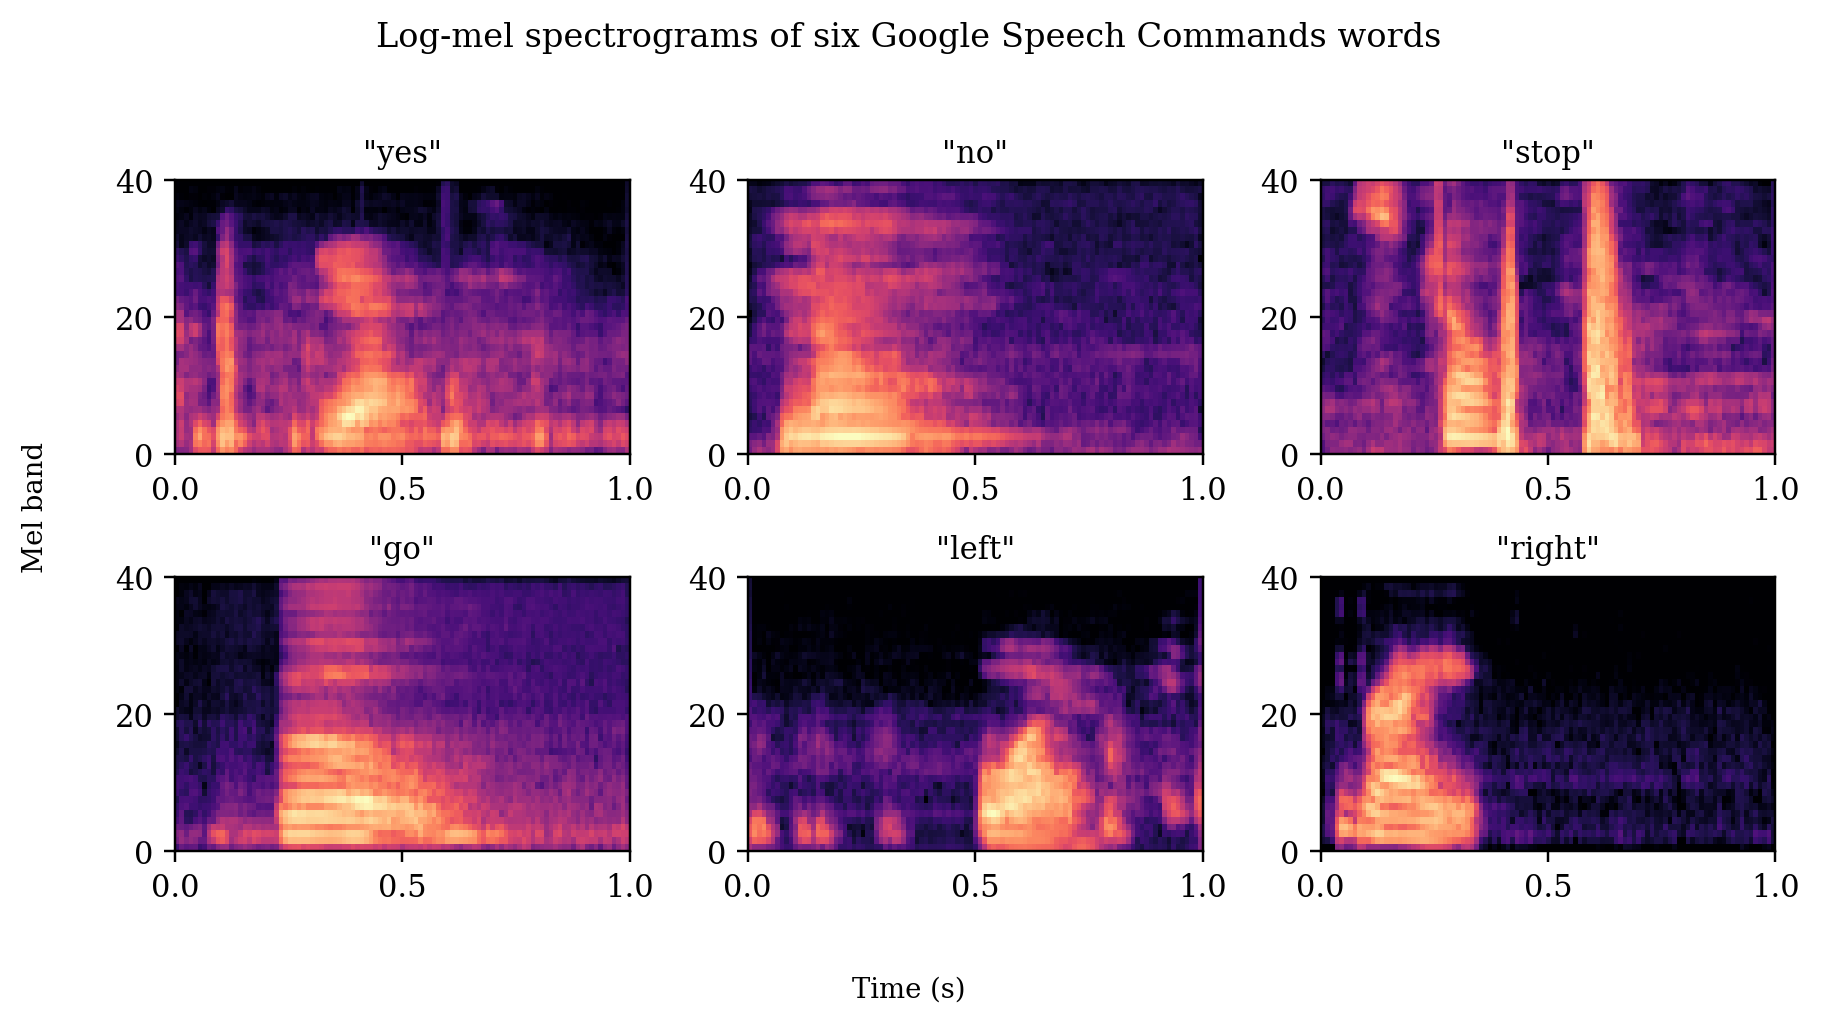
\includegraphics[width=0.95\linewidth]{fig_data_examples.png}
\caption{Log-mel spectrogram của sáu từ lệnh Google Speech Commands (dữ liệu thật).
Các từ khác nhau chiếm các mẫu thời gian--tần số khác nhau rõ ràng --- đây là lý
do khiến học độ đo trong không gian này hiệu quả. \emph{Tạo từ dữ liệu dự án.}}
\label{fig:dataexamples}
\end{figure}

\Cref{fig:melfb} minh họa cụ thể bộ trích xuất mel: (a) 40 bộ lọc tam giác chồng
nhau tổng hợp năng lượng STFT --- dày đặc ở tần số thấp và thưa ở tần số cao ---
và (b) đường cong biến đổi Hz$\to$mel theo \Cref{eq:mel}.

\begin{figure}[H]
\centering
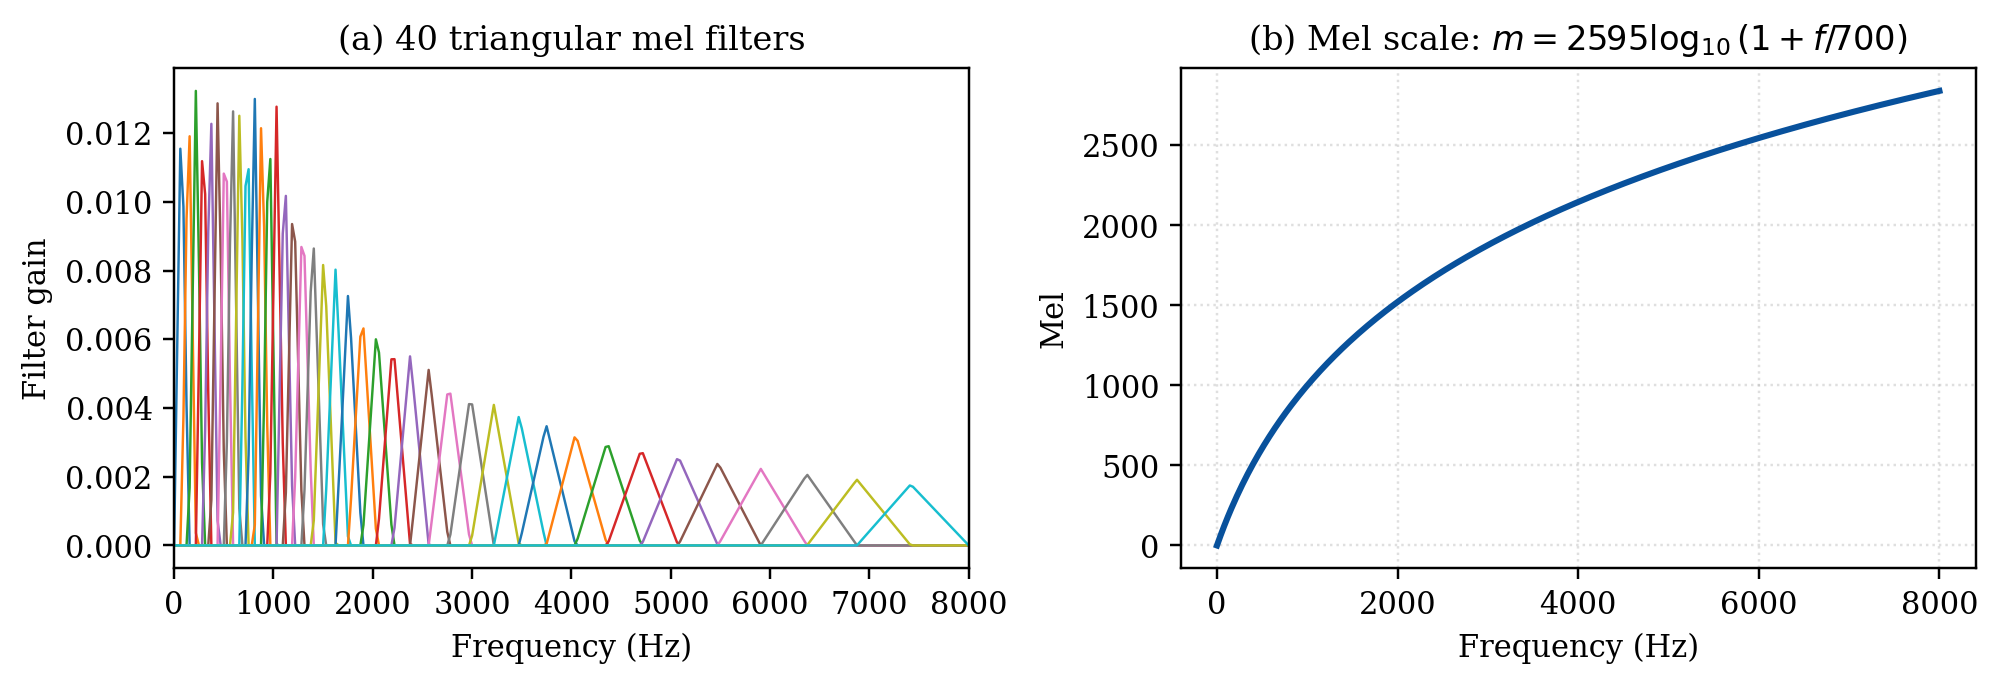
\includegraphics[width=0.95\linewidth]{fig_mel_filterbank.png}
\caption{Bộ trích xuất mel. (a) bộ lọc mel tam giác 40 kênh dùng trong công trình
này; (b) đường cong biến đổi tri giác Hz$\to$mel.}
\label{fig:melfb}
\end{figure}

\section{Nhận Dạng Từ Khóa: Tập Đóng vs.\ Tập Mở}\label{sec:kws-bg}

Nhận dạng từ khóa dấu chân nhỏ (small-footprint KWS) được phổ biến hóa bởi mạng
tích chập phân tách theo chiều sâu (DS-CNN)~\cite{zhang2017hello} và sau đó được
cải tiến bởi mạng broadcasted residual (BC-ResNet)~\cite{kim2021bcresnet}; cả hai
đều đánh đổi độ chính xác lấy số tham số nhỏ để triển khai trên vi điều khiển. Về
bản chất, đây là các bộ phân loại \emph{tập đóng} (closed-set): mô hình xuất ra
một phân phối xác suất trên một tập nhãn \emph{cố định} và luôn chọn nhãn có xác
suất cao nhất.

Hạn chế cốt lõi nằm ở chỗ bộ phân loại tập đóng \emph{không có lựa chọn ``không
thuộc nhãn nào''}. Hàm softmax buộc tổng xác suất trên các lớp đã biết bằng một,
nên mọi đầu vào --- kể cả tiếng ho, tiếng nhạc, hay một từ ngoài danh sách --- đều
bị quy về một trong các từ khóa đã biết. Trong điều kiện phòng thí nghiệm, nơi mọi
mẫu kiểm tra đều thuộc các lớp đã biết, điều này không lộ ra. Nhưng trong thực tế,
đại đa số âm thanh mà thiết bị nghe được \emph{không phải} là từ khóa, nên một bộ
phân loại tập đóng sẽ liên tục gán nhãn nhầm cho âm nền, gây kích hoạt sai.

Bài toán \emph{tập mở} (open-set) đặt ra yêu cầu khó hơn và sát thực tế hơn: hệ
thống phải vừa nhận đúng các từ khóa đã biết, vừa \emph{từ chối} mọi âm thanh
không thuộc tập từ khóa. Thách thức là không gian của ``mọi thứ không phải từ
khóa'' về cơ bản là vô hạn và không thể liệt kê khi huấn luyện, nên không thể coi
nó như một lớp thông thường. Thay vào đó, hệ thống cần một \emph{cơ chế từ chối}:
đo mức độ ``một đầu vào giống các từ khóa đã biết đến đâu'' và bác bỏ khi mức độ
này quá thấp. Khả năng định lượng và điều chỉnh ngưỡng từ chối --- chấp nhận từ
khóa đúng trong khi giữ tỷ lệ kích hoạt nhầm ở mức thấp --- chính là điều phân
biệt một con số độ chính xác trong phòng thí nghiệm với một động cơ từ đánh thức
triển khai được. Đồ án này theo đuổi đúng kịch bản tập mở đó, với cách đo cụ thể
trình bày ở \Cref{sec:eval}.

\section{Học Ít Mẫu và Học Độ Đo}\label{sec:fewshot-bg}

\emph{Học ít mẫu} (few-shot learning) là kịch bản trong đó mô hình phải nhận dạng
một lớp mới chỉ từ một số rất ít ví dụ (vài mẫu, ký hiệu $k$ mẫu). Đây đúng là nhu
cầu của KWS do người dùng định nghĩa: người dùng cung cấp vài mẫu cho mỗi từ khóa
và mong hệ thống nhận dạng được từ đó ngay, không cần huấn luyện lại. Vì không thể
huấn luyện một bộ phân loại mới cho mỗi từ điển, ta cần một cách biểu diễn cho phép
``so khớp'' trực tiếp giữa mẫu mới và vài mẫu đã đăng ký.

Cách tiếp cận tự nhiên là \emph{học độ đo} (metric learning): thay vì học ánh xạ
từ âm thanh sang nhãn cố định, mạng học một \emph{không gian embedding} sao cho
khoảng cách phản ánh sự giống nhau về ngữ nghĩa --- các phát âm của \emph{cùng}
một từ nằm gần nhau, các phát âm của các từ \emph{khác} nhau nằm xa nhau. Khi đã
có không gian như vậy, một từ khóa mới chỉ cần được biểu diễn bằng vị trí của các
mẫu đăng ký, và việc nhận dạng quy về tìm điểm gần nhất --- không phụ thuộc vào
việc từ đó có xuất hiện khi huấn luyện hay không.

Để mô hình học đúng tính chất này, quá trình huấn luyện được tổ chức theo
\emph{phép học} (episodic training): mỗi phép học mô phỏng một bài toán ít mẫu thu
nhỏ bằng cách lấy một nhóm lớp, chia các mẫu của mỗi lớp thành \emph{tập hỗ trợ}
(support, đóng vai mẫu đăng ký) và \emph{tập truy vấn} (query, đóng vai mẫu cần
nhận dạng). Cách tổ chức này khớp với điều kiện triển khai, nên kỹ năng học được
chuyển giao tốt sang lúc sử dụng thật. Mạng prototypical~\cite{snell2017prototypical}
biểu diễn mỗi lớp bằng trung bình (\emph{prototype}) của các embedding hỗ trợ rồi
phân loại truy vấn theo prototype gần nhất; embedding theo triplet~\cite{schroff2015facenet}
lại tối ưu trực tiếp khoảng cách tương đối, kéo cặp cùng lớp lại gần và đẩy cặp
khác lớp ra xa. Hàm mất mát Generalized End-to-End (GE2E)~\cite{wan2018ge2e}, ban
đầu đề xuất cho xác minh người nói, dựng centroid ngay bên trong mỗi batch huấn
luyện đúng như cách triển khai dựng prototype; sự khớp nhau giữa mục tiêu huấn
luyện và quy trình sử dụng khiến GE2E đặc biệt phù hợp với KWS ít mẫu tập mở, và
được đồ án xác nhận bằng thực nghiệm ở \Cref{ch:results}.

\section{Phân Loại Biên Góc và Từ Chối Tập Mở}\label{sec:arc-bg}

Một họ phương pháp khác để học embedding phân biệt cao là \emph{phân loại biên
góc} (angular-margin classification). Ý tưởng là chuẩn hóa cả embedding lẫn vector
trọng số của mỗi lớp về độ dài đơn vị, khiến điểm phân loại trở thành cosine của
góc giữa chúng; sau đó một \emph{biên} (margin) được cộng vào góc của lớp đúng để
ép các lớp tách biệt rõ hơn trên mặt siêu cầu. ArcFace~\cite{deng2019arcface} áp
dụng nguyên lý này và biến thể sub-center SCAF~\cite{deng2020subcenter} cho phép
mỗi lớp có nhiều tâm con, giúp bền vững với dữ liệu nhiễu; cả hai rất thành công
cho nhận dạng khuôn mặt với hàng nghìn danh tính. Vấn đề đặt ra là liệu cơ
chế này có chuyển sang hàng chục nghìn lớp \emph{từ} hay không --- và đây là câu
hỏi mà đồ án trả lời \emph{phủ định} ở quy mô cực lớn (\Cref{ch:results}): khi số
lớp lên tới hàng chục nghìn, số hạng phân loại biên góc lấn át và làm sụp đổ quá
trình học nếu không được giảm trọng số mạnh.

Bên cạnh việc học embedding tốt, KWS tập mở cần một \emph{cơ chế từ chối} để quyết
định khi nào một đầu vào không thuộc bất kỳ từ khóa nào. Cách đơn giản nhất là
ngưỡng theo khoảng cách tới prototype gần nhất (\emph{nearest-class-mean}): chấp
nhận nếu đủ gần, từ chối nếu quá xa. Các phương pháp tinh vi hơn cũng được khảo
sát: OpenMax~\cite{bendale2016openmax} khớp một phân phối đuôi Weibull vào khoảng
cách của từng lớp để ước lượng xác suất ``thuộc về'', còn điểm năng lượng
(energy score)~\cite{liu2020energy} cung cấp một thước đo không cần hiệu chỉnh dựa
trên tổng có trọng số mũ của các khoảng cách. Đồ án điều chỉnh cả hai để hoạt động
trên khoảng cách prototype và so sánh với ngưỡng nearest-class-mean đơn giản
(\Cref{sec:openset}).

Cuối cùng, các mô hình giọng nói tự giám sát như Wav2Vec\,2.0~\cite{baevski2020wav2vec}
được huấn luyện trên lượng lớn dữ liệu không nhãn và cung cấp các biểu diễn rất
mạnh, nhưng quá lớn để chạy trên thiết bị đầu cuối. Vì vậy đồ án dùng Wav2Vec\,2.0
\emph{đóng băng} chỉ như một mô hình \emph{giáo viên} trong \emph{chưng cất kiến
thức} (knowledge distillation): tri thức của giáo viên được truyền sang một bộ mã
hóa \emph{sinh viên} nhỏ gọn, giữ cho mô hình triển khai vẫn rất nhỏ trong khi
hưởng lợi từ biểu diễn của giáo viên (\Cref{sec:losses}).

%==============================================================================
\chapter{Phương Pháp Đề Xuất}\label{ch:method}
\reviewnote{Chương~3 trình bày \emph{những gì đã làm và cách đo lường}, không có
kết quả (kết quả ở Chương~4). Các khối từ bản gốc --- ``Dữ Liệu và Giao Thức'',
``Kiến Trúc Hệ Thống'' và phần phương pháp ``Đánh Giá'' --- được giữ nguyên; văn
bản \textcolor{addcolor}{màu xanh với ký hiệu [+]} là phần thêm mới.}

\NEW{Ở mức cao (\Cref{fig:pipeline}) phương pháp có hai giai đoạn chia sẻ một bộ
mã hóa đóng băng duy nhất. Trong \emph{giai đoạn huấn luyện}, bộ mã hóa được tối
ưu hóa một lần trên MSWC với hàm mục tiêu độ đo. Trong \emph{giai đoạn triển
khai}, người dùng đăng ký vài mẫu mỗi từ khóa để tạo prototype, và truy vấn được
nhận dạng bằng khoảng cách prototype gần nhất với ngưỡng tập mở tường minh ---
bộ mã hóa không bao giờ được huấn luyện lại.}

\begin{figure}[H]
\centering
\resizebox{\linewidth}{!}{%
\begin{tikzpicture}[
  node distance=5mm and 7mm,
  box/.style={draw,rounded corners=2pt,align=center,minimum height=8mm,
              minimum width=15mm,font=\footnotesize,fill=blue!4},
  arr/.style={-{Latex[length=2mm]},thick},
  small/.style={font=\scriptsize,align=center}]
\node[box] (wav) {1\,s âm thanh\\16\,kHz};
\node[box,right=of wav] (feat) {Trích xuất\\đặc trưng\\MFCC/mel$+$PCEN};
\node[box,right=of feat] (enc) {Bộ mã hóa\\$f_\theta$};
\node[box,right=of enc] (norm) {Chuẩn hóa\\$\ell_2$};
\node[box,right=of norm] (proto) {Prototype\\$p_w$};
\node[box,right=of proto] (dist) {Khoảng\\cách gần\\nhất};
\node[box,right=of dist] (dec) {Quyết định\\tập mở};
\draw[arr](wav)--(feat);\draw[arr](feat)--(enc);\draw[arr](enc)--(norm);
\draw[arr](norm)--(proto);\draw[arr](proto)--(dist);\draw[arr](dist)--(dec);
\node[small,below=4mm of proto]{đăng ký\\(ít mẫu)};
\node[small,below=4mm of dist]{truy vấn};
\node[small,below=4mm of dec]{từ khóa /\\\texttt{không biết}};
\begin{scope}[on background layer]
\node[draw,dashed,rounded corners,fit=(wav)(norm),inner sep=3mm,
      label={[font=\scriptsize]above:huấn luyện một lần trên MSWC}]{};
\node[draw,dashed,rounded corners,fit=(proto)(dec),inner sep=3mm,
      label={[font=\scriptsize]above:triển khai (không huấn luyện lại)}]{};
\end{scope}
\end{tikzpicture}}
\caption{\NEW{Pipeline KWS ít mẫu tập mở đầu cuối. Bộ mã hóa được huấn luyện một
lần; khi triển khai, từ khóa người dùng trở thành prototype và truy vấn được phân
loại bằng khoảng cách prototype gần nhất với ngưỡng tập mở.}}
\label{fig:pipeline}
\end{figure}

\section{Phát Biểu Bài Toán}\label{sec:formulation}
\reviewnote{Hình thức hóa ngắn gọn để các phương trình được tham chiếu sau có định
nghĩa rõ ràng.}

Đặt $f_\theta:\R^{T\times F}\!\to\!\R^{d}$ là bộ mã hóa ánh xạ biểu diễn một
giây sang embedding đơn vị chuẩn. Prototype của từ khóa $w$ là trung bình của $k$
embedding hỗ trợ,
\begin{equation}
p_w \;=\; \frac{1}{k}\sum_{i=1}^{k} f_\theta\!\big(x^{(w)}_i\big).
\label{eq:proto}
\end{equation}
Trong \Cref{eq:proto}, $x^{(w)}_i$ là mẫu đăng ký thứ $i$ của từ khóa $w$,
$f_\theta(\cdot)$ là embedding của nó, và $k$ là số mẫu đăng ký (ở đây $k{=}10$).
Ý nghĩa: prototype $p_w$ là ``điểm đại diện trung tâm'' của một từ khóa trong không
gian embedding; lấy trung bình nhiều mẫu giúp khử nhiễu ngẫu nhiên của từng lần
phát âm và cho một mô tả ổn định cho từ đó --- đây chính là thao tác ``đăng ký''
của người dùng.

Truy vấn $x$ được gán cho prototype gần nhất, với điểm tập mở bằng khoảng cách
cực tiểu lấy âm,
\begin{equation}
\hat w(x)=\arg\min_{w} d\!\big(f_\theta(x),p_w\big),\qquad
s(x)=-\!\min_{w} d\!\big(f_\theta(x),p_w\big),
\label{eq:score}
\end{equation}
và được chấp nhận là $\hat w(x)$ nếu $s(x)\ge\tau$, ngược lại được gán nhãn
\texttt{không biết}. Trong \Cref{eq:score}, $d(\cdot,\cdot)$ là khoảng cách trong
không gian embedding và $\tau$ là ngưỡng từ chối. Vế trái xác định \emph{từ khóa
nào} gần nhất; vế phải biến khoảng cách tới prototype gần nhất thành một
\emph{điểm tin cậy} $s(x)$ (gần thì điểm cao, xa thì điểm thấp). Quyết định tập mở
vì vậy rất trực giác: nếu điểm tin cậy vượt ngưỡng $\tau$ thì chấp nhận từ khóa
gần nhất, ngược lại coi đầu vào là ``không biết''. Việc nâng/hạ $\tau$ chính là núm
chỉnh đánh đổi giữa bỏ sót từ khóa và kích hoạt nhầm.

\reviewnote{Hình mới (\ref{fig:embedding}): phép chiếu t-SNE thực của không gian
embedding mô hình đã huấn luyện, tạo bằng cách chạy checkpoint local tốt nhất trên
GSC. Đây là minh họa trực tiếp nhất về lý do tại sao phương pháp hoạt động.}

\Cref{fig:embedding} trực quan hóa không gian học được. Chạy bộ mã hóa đã huấn
luyện tốt nhất trên bản ghi GSC thật và chiếu embedding xuống hai chiều, mỗi lệnh
đã biết tạo thành một cụm chặt, tách biệt quanh prototype của nó (ngôi sao), trong
khi các từ ngoài từ điển (dấu thập xám) nằm ở các khoảng trống giữa các cụm ---
đúng hình học khiến khớp prototype gần nhất với ngưỡng khoảng cách hiệu quả cho
từ chối tập mở.

\begin{figure}[H]
\centering
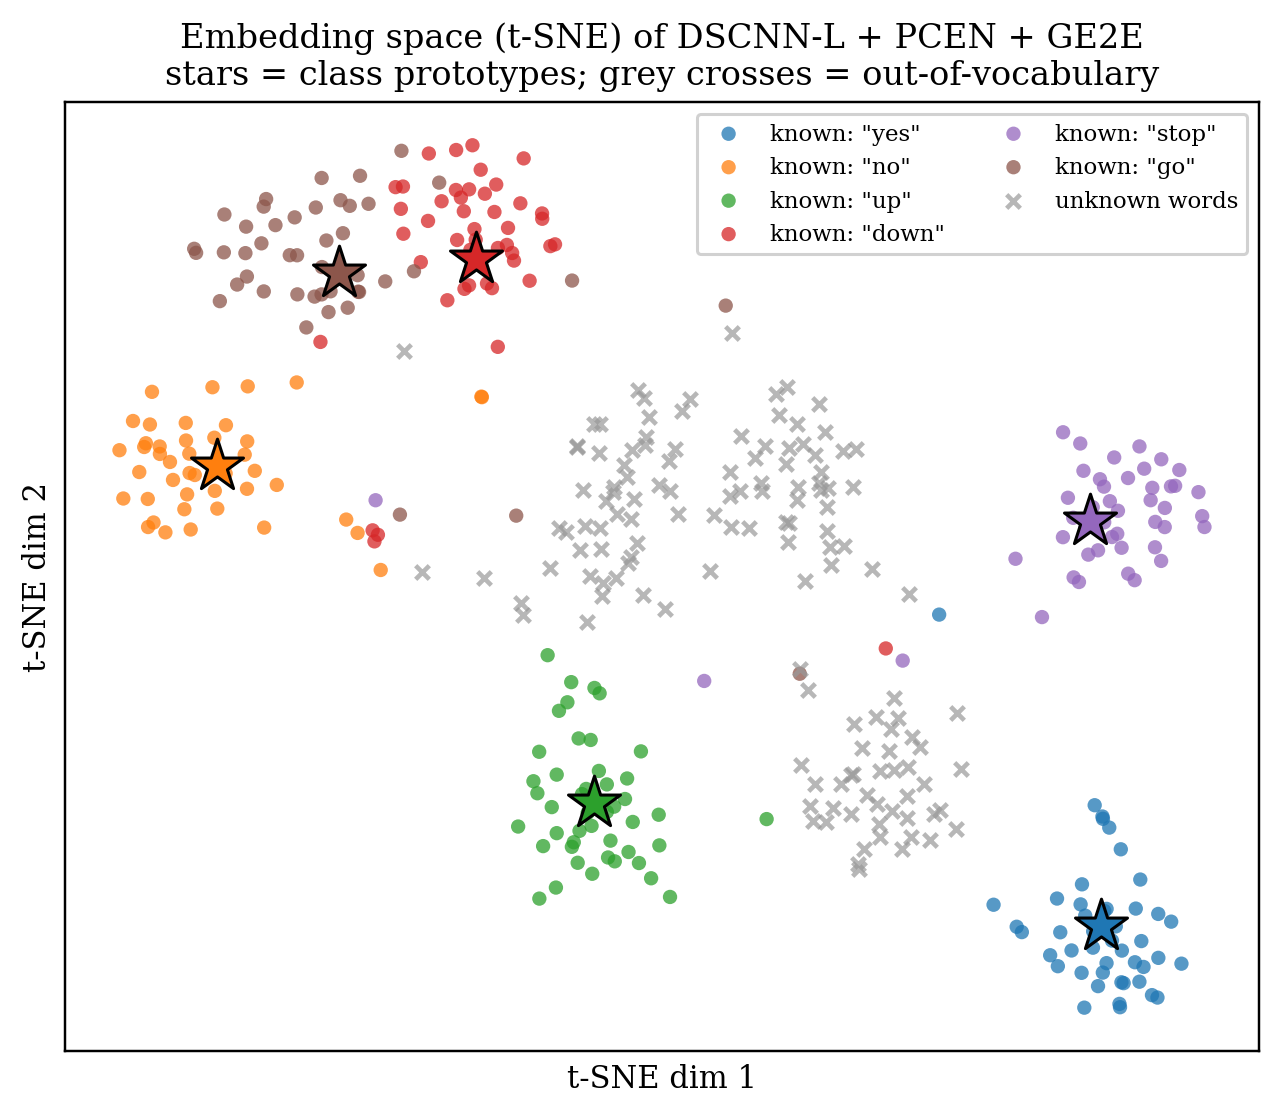
\includegraphics[width=0.68\linewidth]{fig_embedding_space.png}
\caption{\NEW{Chiếu t-SNE embedding từ mô hình DSCNN-L\,+\,PCEN\,+\,GE2E đã
huấn luyện trên audio GSC thật. Điểm màu là sáu lệnh đã biết, ngôi sao là
prototype của chúng, dấu thập xám là từ ngoài từ điển.}}
\label{fig:embedding}
\end{figure}

\reviewnote{Ví dụ minh họa mới --- diễn giải \Cref{eq:proto,eq:score} bằng một tình
huống cụ thể; các con số khoảng cách chỉ mang tính minh họa cho trực giác.}

\paragraph{Ví dụ minh họa: đăng ký, khớp và từ chối.}
Giả sử người dùng muốn thiết bị nhận lệnh ``stop''. \emph{Đăng ký}: người dùng thu
$k{=}10$ clip nói ``stop''; mỗi clip được đưa qua bộ mã hóa thành một embedding, và
trung bình của chúng cho prototype $p_{\text{stop}}$ theo \Cref{eq:proto}. Giả sử
hệ thống chỉ có một từ khóa này và ngưỡng được đặt $\tau$ tương ứng khoảng cách
chấp nhận tối đa $0{,}9$ (tức $s(x)\ge\tau \Leftrightarrow d\le 0{,}9$).
\emph{Khớp}: khi người dùng nói ``stop'', embedding của truy vấn rơi gần
$p_{\text{stop}}$, ví dụ $d=0{,}45$; vì $0{,}45\le 0{,}9$, truy vấn được
\emph{chấp nhận} và gán nhãn ``stop''. \emph{Từ chối}: khi micro thu một âm lạ ---
chẳng hạn một đoạn nhạc hoặc từ ``elephant'' không nằm trong từ điển --- embedding
của nó nằm xa mọi prototype, ví dụ $d=1{,}6$; vì $1{,}6>0{,}9$, hệ thống
\emph{từ chối} và trả về \texttt{không biết} thay vì ép gán nhầm thành ``stop''.
Đúng cơ chế khoảng cách--ngưỡng này, áp dụng đồng thời cho nhiều từ khóa, là nền
tảng cho nhận dạng tập mở của đồ án.

\section{Bộ Dữ Liệu và Giao Thức Huấn Luyện}\label{sec:data}

\textbf{Kho ngữ liệu huấn luyện (MSWC tiếng Anh):} Chúng tôi huấn luyện trên
phân đoạn tiếng Anh của Multilingual Spoken Words Corpus, sau khi lọc theo số
clip tối thiểu chứa 37.387 từ huấn luyện (và 763 từ kiểm định), lấy từ pool
metadata $\sim$38.150 từ và $\sim$6{,}6\,M clip. Để nghiên cứu quy mô, chúng tôi
tạo các giới hạn $\{20, 50, 220, 620\}$ clip mỗi từ --- khoảng $\{0{,}53; 0{,}94;
2{,}05; 2{,}99\}$\,M clip huấn luyện --- và hai chế độ thu nhỏ: phân chia Top-500
truyền thống (450 từ train / 50 từ val, đánh giá trên từ xếp hạng 501+ với
$\ge 1000$ phát âm) và micro-set MLCommons (31 từ khóa) chỉ dùng để xác nhận
pipeline và sàng lọc kiến trúc. \NEW{Ba chế độ từ vựng trải dài hơn ba bậc độ
lớn (\Cref{fig:vocabscale}); phạm vi này là điều khiến các hiệu ứng quy mô ở
\Cref{ch:results} có thể quan sát được.}

\begin{figure}[H]
\centering
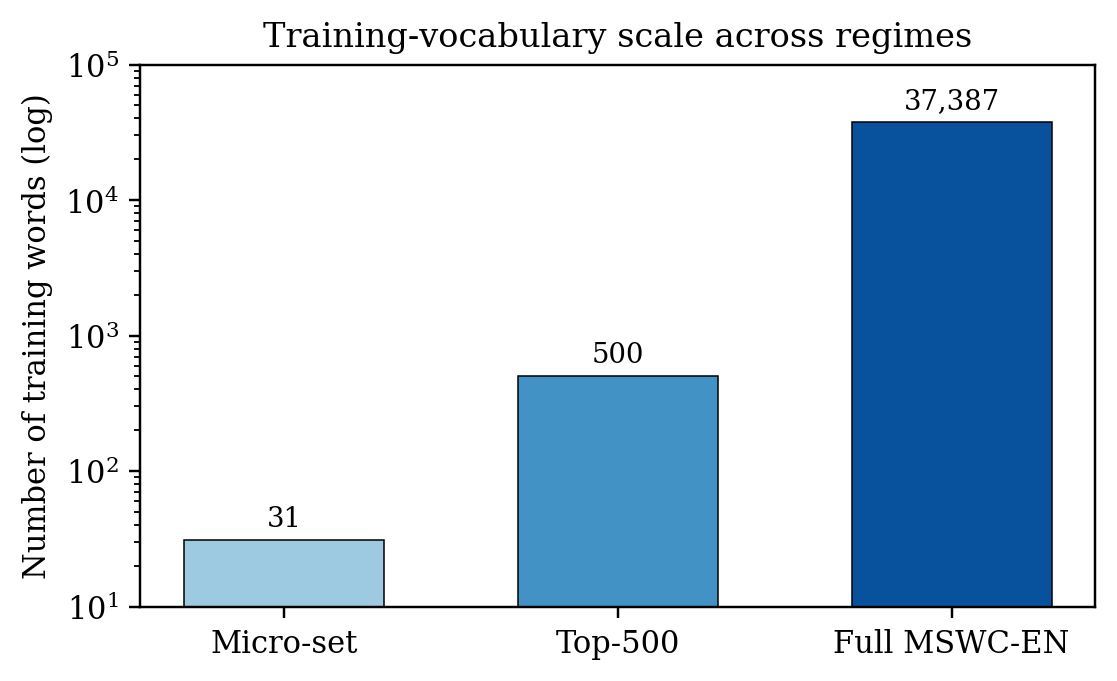
\includegraphics[width=0.72\linewidth]{fig_vocab_scale.png}
\caption{\NEW{Kích thước từ vựng huấn luyện cho ba chế độ (thang lôgarít). Micro-set
chỉ dùng để sàng lọc; MSWC tiếng Anh đầy đủ là chế độ chính.} \emph{Tạo từ dữ
liệu dự án.}}
\label{fig:vocabscale}
\end{figure}

\NEW{Ba chế độ trong \Cref{fig:vocabscale} phục vụ ba mục đích. \emph{Micro-set}
(31 từ) đủ nhỏ để huấn luyện trong vài phút, dùng kiểm tra tính đúng đắn của
pipeline và sàng lọc nhanh các lựa chọn kiến trúc trước khi chạy tốn kém.
\emph{Top-500} là quy mô trung gian theo phân chia truyền thống, cho phép đối
chiếu với các công trình trước dùng cùng thiết lập. \emph{MSWC đầy đủ}
(37.387 từ) là chế độ chính, phản ánh điều kiện thực tế khi từ vựng rất lớn; một
số hiện tượng --- như sự sụp đổ của SCAF ở \Cref{ch:results} --- chỉ bộc lộ ở
quy mô này.}

\textbf{Lấy mẫu theo phép học và tăng cường dữ liệu:} Mỗi phép học lấy 30 lớp
$\times$ 20 phát âm (chỉ các lớp có $\ge 20$ clip mới được chọn). Tăng cường
trực tuyến kết hợp tiếng ồn nền DEMAND (xác suất 0{,}5, SNR lấy mẫu trong
$[0, 10]$\,dB) và áp dụng SpecAugment (một mặt nạ tần số rộng 6, một mặt nạ thời
gian rộng 8); nhiễu khuếch đại ($\pm6$\,dB) và dịch thời gian ($\le 100$\,ms)
được áp dụng với xác suất 0{,}5. \NEW{\Cref{fig:augment} minh họa các tăng cường
này trên bản ghi thật: tiếng ồn nền cộng thêm ở 5\,dB SNR lấp đầy các vùng yên
tĩnh, và các mặt nạ tần số/thời gian của SpecAugment (dải đen) buộc bộ mã hóa
không dựa vào bất kỳ băng hay thời điểm nào.}

\begin{figure}[H]
\centering
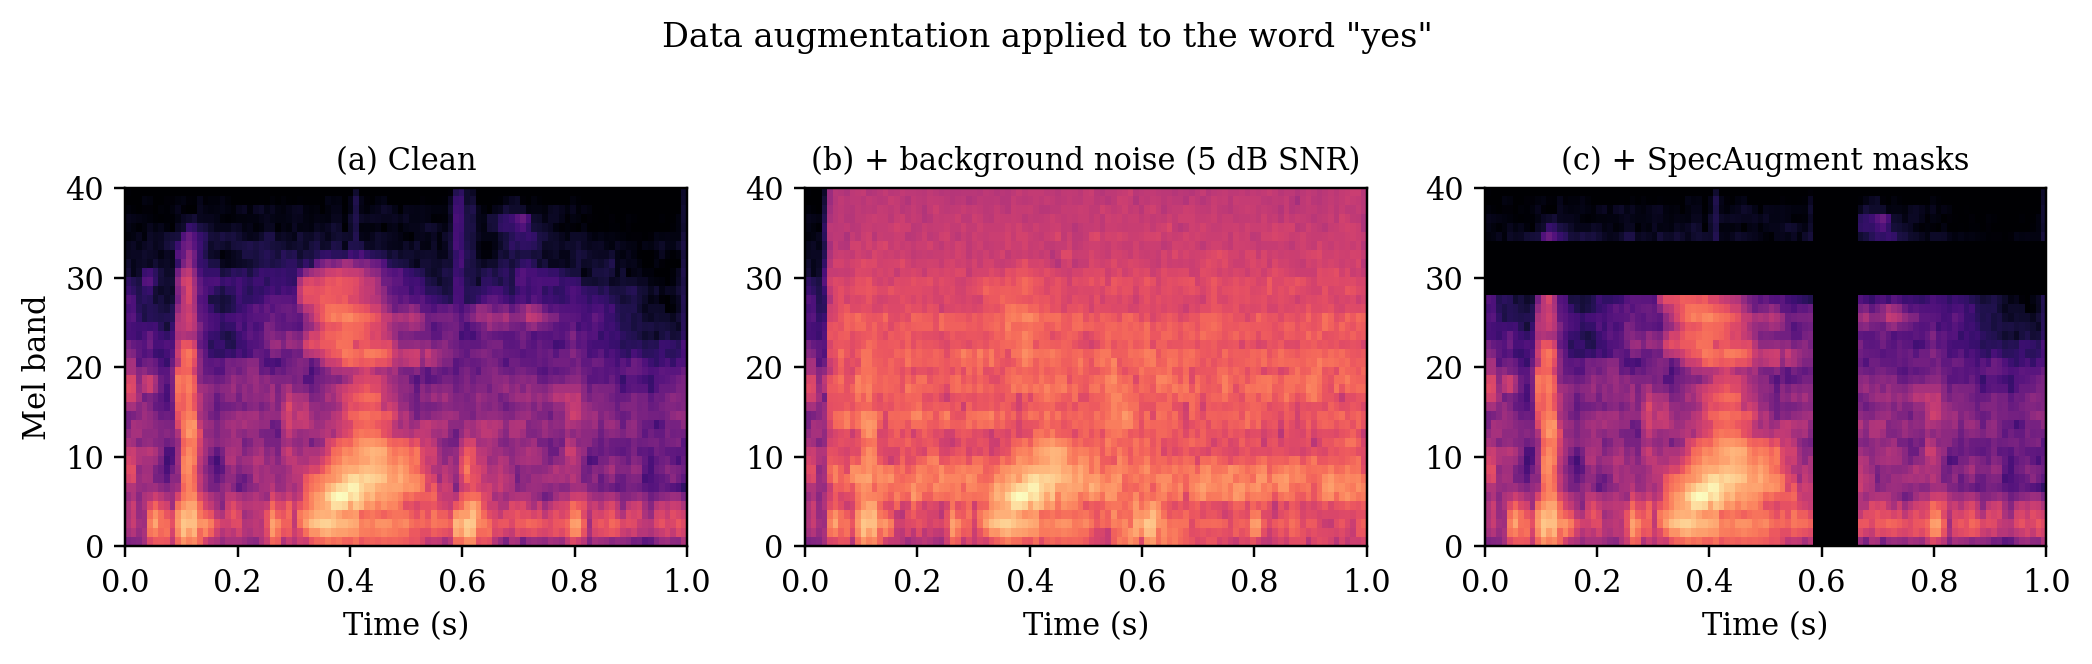
\includegraphics[width=0.98\linewidth]{fig_augmentation.png}
\caption{\NEW{Tăng cường dữ liệu trong huấn luyện trên từ ``yes'' (dữ liệu thật):
(a) log-mel sạch; (b) cộng tiếng ồn nền thật tại 5\,dB SNR; (c) cộng mặt nạ tần
số và thời gian SpecAugment. \emph{Tạo từ dữ liệu dự án.}}}
\label{fig:augment}
\end{figure}

\textbf{Kho ngữ liệu đánh giá (GSC v2):} Chúng tôi đánh giá chéo kho ngữ liệu
trên Google Speech Commands v2. Mẫu đăng ký (hỗ trợ) được lấy từ
\code{validation\_list.txt} chính thức. Mẫu truy vấn được lấy tùy theo phân chia
đánh giá: ở phân chia ``test'', truy vấn lấy từ \code{testing\_list.txt}; ở phân
chia ``dev'', truy vấn lấy từ các file \emph{không} nằm trong
\code{validation\_list.txt} lẫn \code{testing\_list.txt}. Nhờ ba danh sách tách
rời, không có rò rỉ dữ liệu giữa mẫu đăng ký và mẫu truy vấn. Lớp tổng hợp
\code{\_silence\_} được tạo từ các đoạn một giây ngẫu nhiên của
\code{\_background\_noise\_}, với các đoạn không chồng lên nhau cho hỗ trợ và
truy vấn.

\textbf{Giao thức EdgeSpot-exact:} Giao thức chính phân chia 35 từ của GSC thành
11 lớp dương --- mười từ lệnh \{yes, no, up, down, left, right, on, off, stop,
go\} cộng \code{\_silence\_} --- và 25 từ nói âm (không biết). Mỗi lần chạy đăng
ký $k{=}10$ mẫu mỗi từ dương, tính prototype và chấm điểm tối đa 50 mẫu truy
vấn mỗi từ (tập con hạt giống cố định). Chúng tôi báo cáo trung bình$\pm$std qua
100 lần chạy ngẫu nhiên; tính ngẫu nhiên đến từ việc chọn mẫu đăng ký (bản thân
từ điển đã biết/không biết cố định qua các lần chạy).

\reviewnote{Bảng tổng hợp dữ liệu mới (\ref{tab:datasets}): nêu rõ vai trò, nguồn,
quy mô, kích thước đầu vào/đầu ra cho cả hai kho ngữ liệu.}

\begin{table}[H]
\centering
\caption{Tổng hợp hai kho ngữ liệu: MSWC tiếng Anh (huấn luyện) và Google Speech
Commands v2 (đánh giá). Đầu vào và đầu ra của mô hình giống nhau cho cả hai kho do
dùng chung bộ trích xuất đặc trưng.}
\label{tab:datasets}
\small
\setlength{\tabcolsep}{4pt}
\begin{tabular}{p{0.24\linewidth} p{0.38\linewidth} p{0.30\linewidth}}
\toprule
\textbf{Thuộc tính} & \textbf{MSWC tiếng Anh} & \textbf{Google Speech Commands v2}\\
\midrule
Vai trò        & Huấn luyện bộ mã hóa & Đánh giá chéo kho ngữ liệu \\
Nguồn / trích dẫn & Mazumder \emph{và cs.}, 2021~\cite{mazumder2021mswc} &
                 Warden, 2018~\cite{warden2018speech} \\
Số từ (từ vựng) & 37.387 từ huấn luyện / 763 từ kiểm định (pool $\sim$38.150 từ) &
                 35 từ: 11 lớp dương (10 lệnh $+$ \code{\_silence\_}) $+$ 25 từ âm \\
Số clip        & $\sim$6{,}6\,M (metadata); manifest giới hạn $\{20,50,220,620\}$/từ
                 $\to \{0{,}53; 0{,}94; 2{,}05; 2{,}99\}$\,M &
                 $\sim$105\,k phát âm \\
Tần số mẫu     & 16\,kHz, mono & 16\,kHz, mono \\
Độ dài clip    & 1\,s (đệm/cắt thành 16.000 mẫu) & 1\,s (đệm/cắt thành 16.000 mẫu) \\
Đầu vào mô hình & \multicolumn{2}{p{0.70\linewidth}}{Dạng sóng 16.000 mẫu
                 $\to$ đặc trưng $(1,47,10)$ [MFCC] hoặc $(1,40,101)$ [log-mel/PCEN]} \\
Đầu ra mô hình & \multicolumn{2}{p{0.70\linewidth}}{Embedding $d\in\{276,64\}$ đã
                 chuẩn hóa $\ell_2$ $\to$ khoảng cách tới prototype $\to$ từ khóa /
                 \texttt{không biết}} \\
Chế độ sử dụng & Giới hạn $\{20,50,220,620\}$/từ; Top-500 truyền thống; micro-set
                 31 từ (sàng lọc) & EdgeSpot-exact 10 mẫu, chấm tối đa 50 truy
                 vấn/từ, 100 lần chạy \\
\bottomrule
\end{tabular}
\end{table}

\Cref{tab:datasets} tổng hợp hai kho ngữ liệu dùng trong đồ án. Điểm mấu chốt là
\emph{đánh giá chéo kho ngữ liệu}: mô hình được huấn luyện hoàn toàn trên MSWC
tiếng Anh và được kiểm tra trên GSC v2 --- một kho ngữ liệu độc lập về người nói,
thiết bị và từ vựng --- nên kết quả phản ánh khả năng tổng quát hóa thật sự chứ
không phải khớp riêng một bộ dữ liệu.

\section{Kiến Trúc Hệ Thống}\label{sec:arch}

Mục này mô tả ba thành phần cấu thành bộ mã hóa và quy trình quyết định:
\Cref{sec:frontends} trình bày các bộ trích xuất đặc trưng biến dạng sóng thành
biểu diễn thời gian--tần số; \Cref{sec:encoders} mô tả hai kiến trúc bộ mã hóa
(DSCNN-L và EdgeSpot-Full); và \Cref{sec:losses} trình bày các hàm mục tiêu học
độ đo dùng để huấn luyện chúng. Trình tự đi từ tín hiệu đầu vào, qua mạng, đến
embedding mà bộ phân loại triển khai sử dụng.

\subsection{Bộ Trích Xuất Đặc Trưng}\label{sec:frontends}

Tất cả âm thanh là mono, 16\,kHz, được cắt/đệm bằng không thành đúng một giây
(16.000 mẫu). Chúng tôi hỗ trợ hai tham số hóa phổ, tóm tắt ở \Cref{tab:features}.

\begin{table}[H]
\centering
\caption{Các cấu hình bộ trích xuất đặc trưng.}
\label{tab:features}
\begin{tabular}{lcc}
\toprule
 & \textbf{MFCC} & \textbf{Log-mel} \\
\midrule
Tần số mẫu    & \multicolumn{2}{c}{16\,kHz, mono, 1\,s} \\
Kích thước FFT & 1024  & 512  \\
Cửa sổ / bước  & 40/20\,ms & 25/10\,ms \\
\code{center}  & \code{False} & \code{True} \\
Băng mel       & 40 & 40 \\
Hệ số đầu ra   & 10 (DCT đầu tiên) & 40 (mel) \\
Hình dạng tensor & $(1,47,10)$ & $(1,40,101)$ \\
PCEN có thể học & tùy chọn & tùy chọn \\
\bottomrule
\end{tabular}
\end{table}

\textbf{MFCC (frontend cho DSCNN):} Chúng tôi tính 40 hệ số cepstral tần số mel
với FFT 1024 điểm, cửa sổ Hann 640 mẫu (40\,ms), bước 320 mẫu (20\,ms) và
\code{center=False}; bộ lọc mel dùng thang Slaney và chuẩn hóa diện tích Slaney,
log được lấy là $10\log_{10}(\cdot)$ theo sau là DCT-II trực giao. Chỉ giữ 10 hệ
số đầu và hoán vị thành tensor $(1,47,10)=(\text{kênh}, T_{\text{khung}},
\text{đặc trưng})$, trong đó $T = 47 = \lfloor(16000-1024)/320\rfloor + 1$.

\textbf{Log-mel (frontend cho EdgeSpot/BC-ResNet):} Dùng 40 băng mel với FFT 512
điểm, cửa sổ 400 mẫu (25\,ms), bước 160 mẫu (10\,ms) và \code{center=True}, tạo
ra $(1,40,101)$. Nén lôgarít được ủy quyền cho lớp PCEN.

\textbf{PCEN có thể học:} Chuẩn hóa năng lượng theo kênh~\cite{wang2017trainable}
áp dụng bộ làm mượt IIR bậc một nhân quả $M_t = (1-s)M_{t-1} + sE_t$ theo sau là
khuếch đại thích nghi và nén dải động,
\begin{equation}
\text{PCEN}(E_t)=\Big(\frac{E_t}{(\epsilon+M_t)^{\alpha}}+\delta\Big)^{r}-\delta^{r},
\label{eq:pcen}
\end{equation}
với các tham số học được $\alpha,\delta,r,s$ (khởi tạo $0{,}96; 2{,}0; 0{,}5;
0{,}04$; $\epsilon{=}10^{-6}$). Ở \Cref{eq:pcen}, $E_t$ là năng lượng băng mel tại
khung thời gian $t$ và $M_t$ là phiên bản làm mượt theo thời gian của nó (ước
lượng mức nền). Ý nghĩa từng thành phần: phép chia $E_t/(\epsilon+M_t)^{\alpha}$
thực hiện \emph{kiểm soát khuếch đại tự động} --- chuẩn hóa mỗi băng theo mức nền
gần đây nên làm nổi các thay đổi đột ngột (khởi đầu phụ âm) và nén thành phần ổn
định (tiếng ồn nền); số mũ $r$ cùng độ dịch $\delta$ thực hiện \emph{nén dải động}
mềm, thay cho lôgarít tĩnh. Vì $\alpha,\delta,r,s$ được học cùng mạng, PCEN tự
thích nghi với điều kiện ghi âm thay vì dùng một hàm nén cố định --- đây là lý do
nó bền vững hơn và, như \Cref{ch:results} cho thấy, là cải tiến đáng tin cậy nhất.

\reviewnote{Sơ đồ flow tiền xử lý mới (\ref{fig:preproc}): tóm tắt toàn bộ đường
đi từ dạng sóng đến tensor đặc trưng cho cả hai nhánh MFCC và PCEN.}

\begin{figure}[H]
\centering
\begin{tikzpicture}[
  font=\scriptsize, node distance=4mm and 6mm,
  b/.style={draw,rounded corners=1.5pt,align=center,minimum height=8mm,
            minimum width=17mm,fill=blue!4},
  bm/.style={draw,rounded corners=1.5pt,align=center,minimum height=8mm,
            minimum width=17mm,fill=green!6},
  bp/.style={draw,rounded corners=1.5pt,align=center,minimum height=8mm,
            minimum width=17mm,fill=orange!8},
  a/.style={-{Latex[length=1.8mm]}}]
\node[b] (wav) {Dạng sóng\\$16.000$ mẫu\\(16\,kHz, 1\,s)};
\node[b,right=of wav] (stft) {Đóng khung\\$+$ STFT};
\node[b,right=of stft] (mel) {Bộ lọc mel\\40 băng};
\node[bm,above right=2mm and 8mm of mel] (mfcc) {log $+$ DCT\\giữ 10 hệ số};
\node[bp,below right=2mm and 8mm of mel] (pcen) {PCEN\\(học được)};
\node[bm,right=of mfcc] (t1) {Tensor\\$(1,47,10)$};
\node[bp,right=of pcen] (t2) {Tensor\\$(1,40,101)$};
\draw[a](wav)--(stft);\draw[a](stft)--(mel);
\draw[a](mel.east) -- (mfcc.west);
\draw[a](mel.east) -- (pcen.west);
\draw[a](mfcc)--(t1);\draw[a](pcen)--(t2);
\node[font=\scriptsize\itshape,text=green!45!black,above=0.5mm of mfcc]{nhánh MFCC (DSCNN)};
\node[font=\scriptsize\itshape,text=orange!60!black,below=0.5mm of pcen]{nhánh log-mel$+$PCEN (EdgeSpot)};
\end{tikzpicture}
\caption{\NEW{Sơ đồ luồng tiền xử lý: dạng sóng 1\,s $\to$ đóng khung/STFT $\to$ bộ
lọc mel 40 băng $\to$ hai nhánh: log$+$DCT giữ 10 hệ số (MFCC, tensor $(1,47,10)$)
hoặc PCEN học được (log-mel, tensor $(1,40,101)$).}}
\label{fig:preproc}
\end{figure}

\Cref{fig:preproc} tóm tắt toàn bộ pipeline tiền xử lý dưới dạng sơ đồ luồng, từ
dạng sóng một giây tới tensor đặc trưng mà bộ mã hóa nhận vào, với hai nhánh tương
ứng hai bộ trích xuất.

\subsection{Bộ Mã Hóa}\label{sec:encoders}

\reviewnote{Hai sơ đồ khối TikZ mới cho các bộ mã hóa (\ref{fig:dscnn},
\ref{fig:edgespot}) --- tương tự hình kiến trúc của đồ án mẫu nhưng vẽ đúng cho
mạng tùy chỉnh của đồ án này --- cùng hình accuracy-vs-kích thước (\ref{fig:tradeoff}).}

\begin{table}[H]
\centering
\caption{So sánh bộ mã hóa. Chuẩn hóa $\ell_2$ áp dụng ngoài bộ mã hóa để các
hàm mất mát và bộ phân loại triển khai đều hoạt động trên siêu cầu.}
\label{tab:encoders}
\begin{tabular}{lccc}
\toprule
\textbf{Bộ mã hóa} & \textbf{Frontend} & \textbf{$d$} & \textbf{Tham số} \\
\midrule
DSCNN-L              & MFCC / mel($+$PCEN) & 276 & 0{,}413\,M \\
EdgeSpot-Full $\tau{=}4$ & mel($+$PCEN)    & 64  & 0{,}131\,M \\
EdgeSpot-Lite       & mel($+$PCEN)        & 64  & $<0{,}131$\,M \\
BC-ResNet-FS $\tau{=}4$  & mel($+$PCEN)    & 64  & $\sim$0{,}1\,M \\
\bottomrule
\end{tabular}
\end{table}

\textbf{DSCNN-L:} Mạng tích chập phân tách theo chiều sâu xây dựng từ bảng kích
thước: một khối tích chập ban đầu $\text{Conv}(1{\to}276, 10{\times}4, \text{stride
}2{\times}1)$ với đệm ``same'' bất đối xứng kiểu TensorFlow, theo sau là năm khối
phân tách theo chiều sâu (276 kênh, kernel $3{\times}3$; khối đầu strides
$2{\times}2$). Tất cả khối trừ khối cuối dùng BatchNorm+ReLU; khối cuối dùng
LayerNorm (không có affine). Global average pool trực tiếp cho ra embedding nên
chiều embedding bằng chiều rộng kênh, $d = 276$. DSCNN-L có $\approx 0{,}413$\,M
tham số.

\begin{figure}[H]
\centering
\begin{tikzpicture}[
  font=\scriptsize, node distance=3.2mm,
  b/.style={draw,rounded corners=1.5pt,minimum height=7mm,align=center,fill=blue!5},
  a/.style={-{Latex[length=1.6mm]}}]
\node[b] (in) {đầu vào\\$(1,47,10)$};
\node[b,right=of in] (c0) {Conv\\$10{\times}4$\\s$2{\times}1$,\,276\\BN+ReLU};
\node[b,right=of c0] (d1) {DS-Blk1\\$3{\times}3$\\s$2{\times}2$};
\node[b,right=of d1] (d2) {DS-Blk\\2--4\\$3{\times}3$};
\node[b,right=of d2] (d5) {DS-Blk5\\$3{\times}3$\\+LayerNorm};
\node[b,right=of d5] (gap) {GAP};
\node[b,right=of gap] (emb) {emb\\$d{=}276$};
\draw[a](in)--(c0);\draw[a](c0)--(d1);\draw[a](d1)--(d2);\draw[a](d2)--(d5);
\draw[a](d5)--(gap);\draw[a](gap)--(emb);
\end{tikzpicture}
\caption{\NEW{Sơ đồ khối DSCNN-L: CNN phân tách theo chiều sâu, $\approx$0{,}41\,M
tham số. Embedding bằng chiều rộng kênh cuối (276); không có phép chiếu tuyến
tính.}}
\label{fig:dscnn}
\end{figure}

\textbf{EdgeSpot-Full ($\tau{=}4$):} Bộ mã hóa cạnh thu nhỏ chiều rộng hoạt động
trên đầu vào mel/PCEN $(1,40,101)$. Một stem $5{\times}5$ stride-$(2,1)$ cấp cho
bốn giai đoạn khối fused-temporal và broadcasted-residual ``lite'' với giãn thời
gian tăng dần $(1,2,4,8)$; một khối sụp đổ tần số theo chiều sâu lấy trung bình
tần số thành chuỗi $(C,T)$; một tích chập vị trí theo chiều sâu và một khối chú ý
thời gian đơn đầu ($d = 64$) mô hình hóa cấu trúc thời gian tầm xa; cuối cùng
một đầu thời gian theo chiều sâu và global pooling tạo ra embedding 64 chiều.
EdgeSpot-Full $\tau{=}4$ có $\approx 0{,}131$\,M tham số, nhỏ hơn DSCNN-L
$\sim$3{,}2 lần.

\begin{figure}[H]
\centering
\begin{tikzpicture}[
  font=\scriptsize, node distance=2.6mm,
  b/.style={draw,rounded corners=1.5pt,minimum height=7mm,align=center,fill=orange!8},
  a/.style={-{Latex[length=1.6mm]}}]
\node[b] (in) {đầu vào\\$(1,40,101)$};
\node[b,right=of in] (pc) {PCEN};
\node[b,right=of pc] (st) {Stem\\$5{\times}5$\\s$(2,1)$};
\node[b,right=of st] (s12) {Giai đoạn 1--2\\Fused-Temporal\\giãn 1,2};
\node[b,right=of s12] (s34) {Giai đoạn 3--4\\BCRes-Lite\\giãn 4,8};
\node[b,below=5mm of s34] (fc) {Sụp đổ\\tần số};
\node[b,left=of fc] (att) {Pos-Conv\\$+$chú ý\\1 đầu};
\node[b,left=of att] (th) {Đầu thời\\gian + GAP};
\node[b,left=of th] (emb) {emb\\$d{=}64$};
\draw[a](in)--(pc);\draw[a](pc)--(st);\draw[a](st)--(s12);\draw[a](s12)--(s34);
\draw[a](s34)--(fc);\draw[a](fc)--(att);\draw[a](att)--(th);\draw[a](th)--(emb);
\end{tikzpicture}
\caption{\NEW{Sơ đồ khối EdgeSpot-Full ($\tau{=}4$): frontend mel/PCEN, các khối
fused-temporal và broadcasted-residual với giãn tăng dần, sụp đổ tần số, giai đoạn
chú ý thời gian một đầu, $\approx$0{,}13\,M tham số.}}
\label{fig:edgespot}
\end{figure}

\subsection{Các Hàm Mục Tiêu Học Độ Đo}\label{sec:losses}

Tất cả hàm mục tiêu được huấn luyện theo phép học: mỗi phép học lấy mẫu
$n_{\text{cls}}{=}30$ lớp với $n_{\text{spp}}{=}20$ phát âm mỗi lớp (600
embedding/phép học).

\begin{figure}[H]
\centering
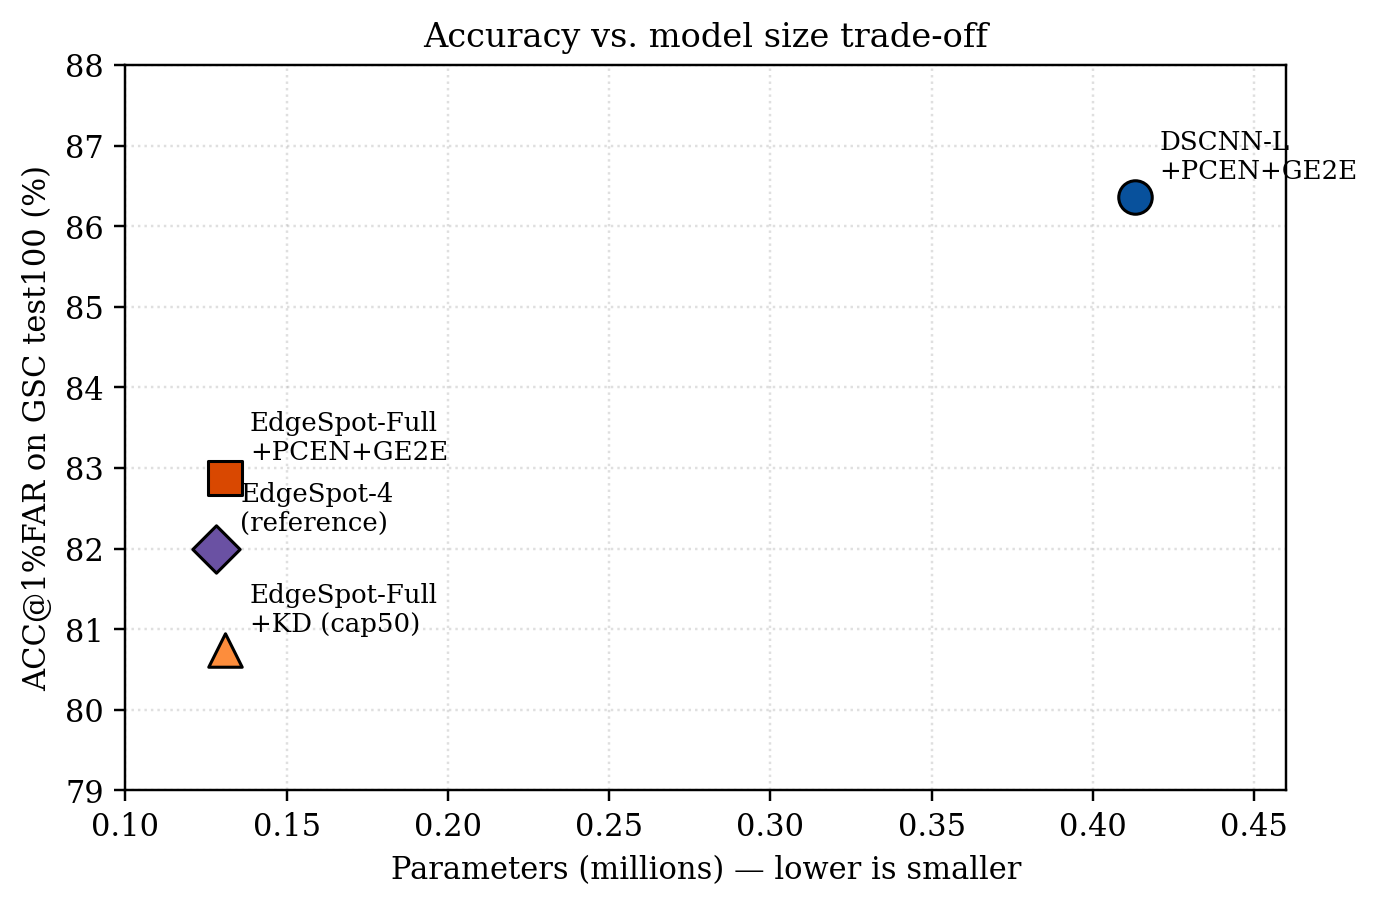
\includegraphics[width=0.78\linewidth]{fig_model_tradeoff.png}
\caption{\NEW{Đánh đổi độ chính xác vs.\ kích thước mô hình. DSCNN-L dẫn đầu về
độ chính xác; EdgeSpot-Full đạt điểm cạnh tranh với một phần ba tham số; KD nâng
mô hình nhỏ gọn ở dữ liệu ít. (Số liệu chi tiết ở \Cref{ch:results}.)} \emph{Tạo
từ kết quả dự án.}}
\label{fig:tradeoff}
\end{figure}

\textbf{Triplet:} Hàm mất mát triplet bán-khó~\cite{schroff2015facenet} với
khoảng cách Euclid, $\mathcal{L}=\frac{1}{N}\sum\max(0, d(a,p)-d(a,n)+m)$, với
khai thác positive khó nhất và khai thác negative bán-khó kiểu FaceNet. Ở đây $a$
là mẫu neo, $p$ là mẫu \emph{cùng} từ (positive), $n$ là mẫu \emph{khác} từ
(negative) và $m$ là biên. Ý nghĩa: hàm này ép khoảng cách neo--positive nhỏ hơn
khoảng cách neo--negative ít nhất một lượng $m$; phần $\max(0,\cdot)$ nghĩa là chỉ
phạt khi điều kiện chưa thỏa, tức chỉ học từ các bộ ba ``khó''.

\textbf{Sub-center ArcFace (SCAF):} Softmax biên góc cộng với $K{=}3$ sub-center
mỗi lớp. Logit mỗi lớp là max cosine qua các sub-center,
$\cos\theta_c = \max_{j\le K} w_{c,j}^{\top} z$; biên cộng $m{=}0{,}5$ áp dụng
cho lớp đích và logit được nhân $s{=}30$ trước cross-entropy. Ý nghĩa: $z$ là
embedding chuẩn hóa, $w_{c,j}$ là tâm con thứ $j$ của lớp $c$; lấy max qua các tâm
con cho phép một từ có nhiều ``kiểu phát âm'' khác nhau. Biên $m$ buộc lớp đúng
phải vượt trội rõ rệt về góc, còn thang $s$ khuếch đại điểm trước softmax --- chính
hai yếu tố này, khi nhân lên hàng chục nghìn lớp, gây ra hiện tượng sụp đổ phân
tích ở \Cref{ch:results}.

\textbf{GE2E (centroid):} Hàm mất mát generalized end-to-end~\cite{wan2018ge2e}
phản ánh triển khai: trong mỗi phép học mỗi lớp được chia thành hỗ trợ/truy vấn;
centroid là trung bình hỗ trợ chuẩn hóa $\ell_2$ và truy vấn được phân loại bằng
cosine similarity có thang và bias học được, tối ưu hóa bằng cross-entropy. GE2E
trực tiếp tối ưu hóa mục tiêu đăng ký-rồi-khớp của \Cref{eq:proto,eq:score}.

\textbf{Chưng cất cosine (KD):} Chúng tôi thêm chưng cất từ mô hình giáo viên
Wav2Vec\,2.0-base đóng băng (lớp ẩn 16, mean-pooled, chiếu sang $d{=}64$ bởi đầu
sub-center-ArcFace đã huấn luyện). Hàm mất mát chưng cất là thuần cosine embedding,
\begin{equation}
\mathcal{L}_{\text{KD}} = 1 - \frac{1}{N}\sum_i
\cos\!\big(f_\theta(x_i),\, g_{\text{giáo viên}}(x_i)\big),
\label{eq:kd}
\end{equation}
không có nhiệt độ/nhãn mềm. Trong \Cref{eq:kd}, $f_\theta(x_i)$ là embedding của
mô hình sinh viên và $g_{\text{giáo viên}}(x_i)$ là embedding của mô hình giáo viên
Wav2Vec\,2.0 đã đóng băng cho cùng đầu vào $x_i$. Ý nghĩa: vì $\cos$ bằng 1 khi hai
vector cùng hướng, cực tiểu hóa $\mathcal{L}_{\text{KD}}$ tương đương kéo embedding
sinh viên \emph{cùng hướng} với embedding giáo viên --- tức ép mô hình nhỏ bắt
chước không gian biểu diễn của mô hình lớn. Embedding giáo viên được tính trước
offline và tra cứu theo đường dẫn file khi huấn luyện, nên chi phí huấn luyện thêm
là không đáng kể.

\textbf{Kết hợp lai:} Chúng tôi tạo tổng có trọng số, ví dụ \code{scaf\_ge2e},
\code{kd\_ge2e}, \code{kd\_scaf}, \code{kd\_scaf\_ge2e}. Một chi tiết triển khai
quan trọng (và là phát hiện thực nghiệm chính, \Cref{ch:results}) là trọng số
SCAF: trong KD được đặt là $5\times10^{-5}$ trong khi trọng số GE2E/KD là 1{,}0.

\NEW{\textbf{Tối ưu hóa.} Trừ khi ghi chú khác, mọi mô hình được huấn luyện bằng
thuật toán Adam với tốc độ học khởi đầu $10^{-3}$ và hệ số phạt trọng số (weight
decay) $10^{-4}$. Chuẩn của gradient được cắt ở ngưỡng $5{,}0$ (gradient clipping)
để tránh các bước cập nhật quá lớn gây mất ổn định, nhất là với các hàm mất mát
lai. Tốc độ học giảm dần theo lịch \emph{cosine annealing kèm khởi động lại}
(CosineAnnealingWarmRestarts): giá trị tốc độ học đi xuống theo đường cong cosine
rồi được đặt lại theo chu kỳ, với chu kỳ đầu dài $T_0{=}10$ epoch, mỗi chu kỳ kế
tiếp dài gấp $T_{\text{mult}}{=}2$ lần chu kỳ trước, và mức sàn
$\eta_{\min}{=}10^{-5}$. Để kết quả có thể tái lập, chúng tôi cố định mọi hạt giống
ngẫu nhiên ($=42$) và bật chế độ tính toán tất định của thư viện cuDNN.}

\section{Các Đầu Từ Chối Tập Mở}\label{sec:openset}
\reviewnote{Mục mới mô tả bốn đầu từ chối đã triển khai.}

Tất cả các đầu chia sẻ giao diện prototype và chỉ khác nhau ở điểm từ chối; từ
khóa dự đoán luôn là lớp argmin khoảng cách (\Cref{eq:score}).
(i) \textbf{Nearest-class-mean (NCM, ``L2 trực tiếp'')} --- mặc định của chúng
tôi --- từ chối khi khoảng cách prototype tối thiểu vượt ngưỡng, dùng khoảng cách
thô không chuẩn hóa xác suất.
(ii) \textbf{OpenMax}~\cite{bendale2016openmax} khớp đuôi Weibull với khoảng cách
hỗ trợ-tới-prototype và dùng $1-\text{CDF}$ làm điểm thành viên.
(iii) \textbf{Energy}~\cite{liu2020energy} xem $-d_i$ như logit và dùng năng
lượng tự do $E(x)=T\log\sum_i\exp(-d_i/T)$ làm điểm chấp nhận.
(iv) \textbf{Ngưỡng hiệu chỉnh} ($\mu+2\sigma$ của khoảng cách hỗ trợ) điều
khiển bảng phân tích nhầm lẫn theo từng từ.

\section{Phương Pháp Đánh Giá}\label{sec:eval}

Mục này định nghĩa các chỉ số đánh giá \emph{trước khi} chúng được dùng ở
\Cref{ch:results}. Chúng tôi xem bài toán tập mở là phát hiện nhị phân từ khóa
vs.\ không phải từ khóa kết hợp theo dõi danh tính đa lớp, và xây dựng tất cả chỉ
số trên đường cong ROC. Trước hết, hai khái niệm cơ sở: \far{} (False-Accept
Rate) là tỷ lệ âm thanh \emph{không phải} từ khóa bị chấp nhận nhầm, và \frr{}
(False-Reject Rate) là tỷ lệ từ khóa \emph{thật} bị từ chối nhầm. Ký hiệu
$\uparrow$ nghĩa là \emph{cao hơn tốt hơn}, $\downarrow$ nghĩa là \emph{thấp hơn
tốt hơn}.
\begin{itemize}[leftmargin=1.3em,itemsep=1pt]
\item \textbf{AUC} ($\uparrow$): diện tích dưới ROC của điểm tập mở
(\Cref{eq:score}); không phụ thuộc ngưỡng, đo khả năng phân tách từ khóa với
không-từ-khóa nói chung.
\item \textbf{EER} ($\downarrow$): tỷ lệ lỗi bằng nhau, điểm hoạt động tối thiểu
hóa $|\far-\frr|$, báo cáo là $(\far+\frr)/2$.
\item \textbf{FRR@FAR} ($\downarrow$): tỷ lệ từ chối sai tại ngưỡng lớn nhất có tỷ
lệ chấp nhận sai không vượt mục tiêu (1\% hoặc 5\%).
\item \textbf{Open-set ACC@FAR} ($\uparrow$): độ chính xác chính. Truy vấn đã biết
đúng khi được chấp nhận ($s\ge\tau_{\far}$) và nhãn argmin đúng; truy vấn không
biết đúng khi bị từ chối. Báo cáo tại $\far\in\{1\%, 5\%\}$.
\item \textbf{Keyword ACC} ($\uparrow$): độ chính xác prototype gần nhất tập đóng
chỉ trên truy vấn đã biết (bỏ qua từ chối).
\item \textbf{F1} ($\uparrow$): F1 nhị phân từ khóa vs.\ không biết tại ngưỡng EER.
\end{itemize}

\section{Thiết Kế Thực Nghiệm: Những Gì Chúng Tôi Đo}\label{sec:expdesign}
\reviewnote{Mục mới. Phát biểu bốn câu hỏi thực nghiệm sẽ trả lời (không có kết
quả --- kết quả ở Chương~4).}

Các thực nghiệm được tổ chức quanh bốn câu hỏi:
\begin{description}[leftmargin=1.6em,itemsep=2pt]
\item[\textbf{Q1 --- Trục thiết kế nào quan trọng?}] Chúng tôi huấn luyện tất cả
$2{\times}2{\times}4 = 16$ tổ hợp \{DSCNN-L, EdgeSpot-Full\} $\times$
\{MFCC, PCEN\} $\times$ \{Triplet, SCAF, GE2E, SCAF$+$GE2E\} và cô lập từng trục.
\item[\textbf{Q2 --- Hiệu suất quy mô như thế nào?}] Cố định frontend/loss tốt
nhất, chúng tôi quét giới hạn $\{20,50,220,620\}$ và tăng từ vựng từ 31 đến
37.387 từ.
\item[\textbf{Q3 --- Chưng cất có thể thay thế dữ liệu không?}] Chúng tôi so sánh
GE2E với hàm mục tiêu cosine-KD ở các giới hạn dữ liệu tương đương.
\item[\textbf{Q4 --- Hệ thống triển khai tốt nhất là gì?}] Chúng tôi tổng hợp các
cấu hình mạnh nhất theo từng chế độ dữ liệu.
\end{description}

\section{Triển Khai: Phát Trực Tuyến và Bản Demo}\label{sec:deploy}
\reviewnote{Mục mới mô tả pipeline trên thiết bị/phát trực tuyến và web demo.}

Ngoài bộ mã hóa lõi, hệ thống bao gồm pipeline phát trực tuyến trên CPU và bản
demo web offline (\Cref{fig:demo}). Phát trực tuyến thực hiện phát hiện cửa sổ trượt (cửa sổ 1\,s,
bước 0{,}5\,s) được kiểm soát bởi Silero VAD: chỉ các cửa sổ VAD đánh dấu là lời
nói mới được nhúng và khớp. Một \emph{máy trạng thái} quyết định không phụ thuộc
backend (\Cref{alg:sm}) ổn định các ứng viên thô thành sự kiện sạch bằng bầu chọn
đa số ngắn, kiểm tra biên top-2 và thời gian hồi phục để ngăn kích hoạt trùng lặp.
Các module tùy chọn --- bộ giảm nhiễu spectral-gating/SpeechBrain và cổng xác minh
người nói ECAPA-TDNN --- tuân theo cùng mô hình fail-open, bật/tắt runtime.

\begin{algorithm}[H]
\caption{Máy trạng thái quyết định phát trực tuyến (làm mượt $+$ hồi phục).}
\label{alg:sm}
\footnotesize
\begin{algorithmic}[1]
\Require cửa sổ $W$, phiếu $V$, biên $m_{\min}$, hồi phục $C$
\State bộ đệm $\gets$ deque(maxlen $=W$);\ $t_{\text{cuối}}\gets-\infty$
\For{mỗi ứng viên $c$ với khoảng $[t_s,t_e]$}
  \If{$t_s - t_{\text{cuối}} < C$} \State phát \textsc{hồi\_phục};\ \textbf{tiếp tục} \EndIf
  \If{$\lnot c.\text{phát hiện}$ \textbf{hoặc} $c.\text{kw}{=}$\texttt{không biết}
       \textbf{hoặc} $c.\text{biên}<m_{\min}$}
     \State xóa bộ đệm; phát \textsc{từ\_chối};\ \textbf{tiếp tục}
  \EndIf
  \State đẩy $c$;\ $k^\star\gets$ từ khóa đa số trong bộ đệm
  \If{phiếu$(k^\star)\ge V$}
     \State $a\gets\arg\max_{\text{độ tin}}$\{$c\in$bộ đệm: $c.\text{kw}{=}k^\star$\}
     \State $t_{\text{cuối}}\gets a.t_e$; xóa bộ đệm; phát \textsc{phát\_hiện}$(k^\star)$
  \Else\ \State phát \textsc{đang\_chấm\_điểm} \EndIf
\EndFor
\end{algorithmic}
\end{algorithm}

\begin{figure}[H]
\centering
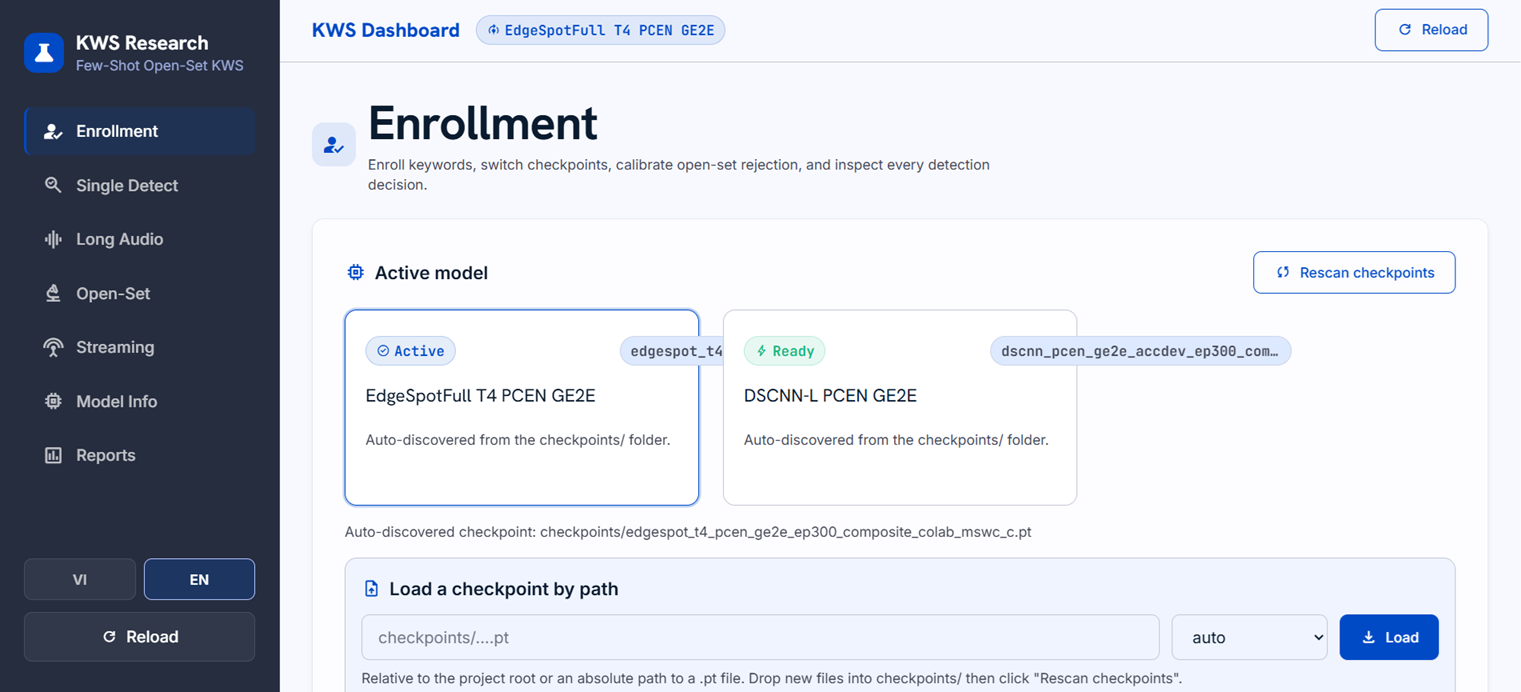
\includegraphics[width=0.95\linewidth]{homepage.png}
\caption{\NEW{Bản demo web offline: bộ chuyển đổi mô hình và khung xem thời điểm
trên audio dài, trong đó các từ khóa được phát hiện được đánh dấu dọc theo bản
ghi. \emph{Ảnh chụp màn hình demo của dự án.}}}
\label{fig:demo}
\end{figure}

%==============================================================================
\chapter{Kết Quả và Phân Tích}\label{ch:results}
\reviewnote{Toàn bộ chương này là mới. Báo cáo và phân tích các số đo, tham chiếu
đến hình kết quả trong \code{assets/}.}

Chương này trình bày và phân tích kết quả thực nghiệm; các chỉ số đã được định
nghĩa ở \Cref{sec:eval}, nên ở đây chỉ thuần phân tích con số. \Cref{sec:res-train}
trước hết kiểm tra diễn biến huấn luyện để xác nhận quá trình tối ưu lành mạnh.
Sau đó, kết quả được tổ chức đúng theo bốn câu hỏi nghiên cứu đã nêu ở
\Cref{sec:expdesign}: \Cref{sec:res-q1} (Q1) cô lập trục thiết kế nào quan trọng;
\Cref{sec:res-q2} (Q2) phân tích hiệu ứng quy mô, gồm cả bão hòa dữ liệu và sụp đổ
SCAF; \Cref{sec:res-q3} (Q3) xét chưng cất có thể thay một phần dữ liệu hay không;
và \Cref{sec:res-q4} (Q4) tổng hợp các hệ thống triển khai tốt nhất. Cuối cùng,
\Cref{sec:res-inference} kiểm chứng đầu cuối trên bản ghi dài.

\paragraph{Quy ước báo cáo.} Trừ khi ghi rõ, mọi số liệu là trung bình$\pm$độ lệch
chuẩn (std) qua giao thức EdgeSpot-exact 10 mẫu với 100 lần chạy trên GSC test (ký
hiệu \emph{test100}); độ lệch chuẩn phản ánh độ ổn định giữa các lần chọn mẫu đăng
ký. Số tốt nhất mỗi cột được \best{in đậm}. Theo quy ước ở \Cref{sec:eval}, cao hơn
tốt hơn cho ACC/AUC/F1/Keyword-ACC và thấp hơn tốt hơn cho EER/FRR. Các dòng được
đánh dấu ``sụp.'' là cấu hình bị sụp đổ suy biến ($\auc{\approx}50$, F1$\approx$0,
$\frr{\approx}100\%$) và \emph{không} được coi là kết quả tốt dù ACC tập mở quanh
$69\%$ (đó là hành vi từ chối-tất-cả).

\section{Diễn Biến Huấn Luyện}\label{sec:res-train}
\reviewnote{Mục mới. \Cref{fig:traincurves} được vẽ từ \emph{log TensorBoard local
thật} (không cần huấn luyện lại), tương tự hình ``Loss Huấn Luyện và Kiểm Định''
của đồ án mẫu.}

\Cref{fig:traincurves} cho thấy quỹ đạo huấn luyện thực sự của mô hình neo
Microset (EdgeSpot-Full + SCAF+GE2E), đọc trực tiếp từ log TensorBoard đã lưu.
Hàm mất mát SCAF+GE2E giảm mượt từ $\sim$15{,}5 xuống $\sim$1{,}3, AUC kiểm định
tăng lên và ổn định gần $98\%$, độ chính xác tập mở GSC-dev đạt ngưỡng $\sim$85\%
--- một quỹ đạo lành mạnh, không bị overfit.

\begin{figure}[H]
\centering
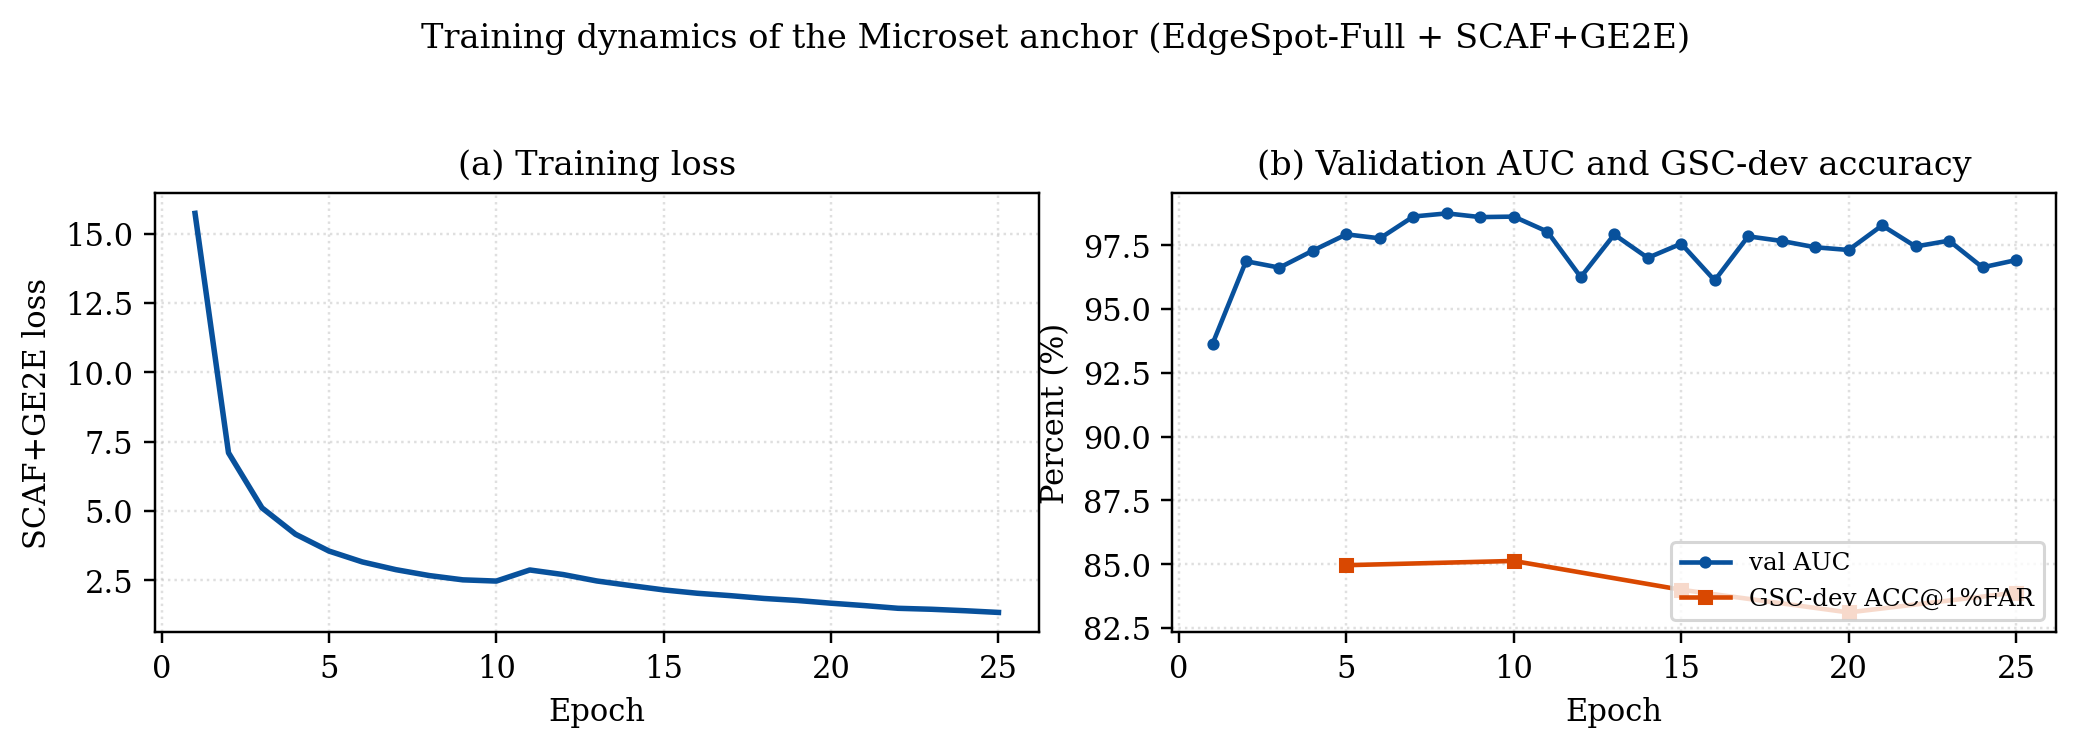
\includegraphics[width=0.98\linewidth]{fig_training_curves.png}
\caption{\NEW{Diễn biến huấn luyện thực sự của mô hình neo Microset (EdgeSpot-Full
+ SCAF+GE2E), từ log TensorBoard local: (a) hàm mất mát huấn luyện; (b) AUC kiểm
định và GSC-dev ACC@1\%FAR theo epoch.}}
\label{fig:traincurves}
\end{figure}

\section{Q1: Trục Thiết Kế Nào Quan Trọng}\label{sec:res-q1}

\begin{table}[H]
\centering
\caption{Bộ sàng lọc 16 cấu hình đầy đủ trên MSWC toàn từ vựng (cap-620),
GSC test100 @ 1\% FAR. Giá trị là trung bình$\pm$std qua 100 lần chạy.
``sụp.'' đánh dấu sụp đổ suy biến ($\auc{=}50$, $\text{F1}{=}0$, $\frr{=}100\%$);
std$=0$ ở các dòng này phản ánh hành vi từ chối-tất-cả mang tính tất định. Tốt
nhất in đậm.}
\label{tab:matrix}
\scriptsize
\setlength{\tabcolsep}{3pt}
\begin{tabular}{lll r r r r}
\toprule
\textbf{Bộ mã hóa} & \textbf{Đặc trưng} & \textbf{Loss} &
\acc$_{1\%}$ & \auc & \eer & F1\\
\midrule
DSCNN & MFCC & Triplet     & 71{,}52$\pm$0{,}67 & 75{,}55$\pm$1{,}09 & 31{,}41$\pm$0{,}98 & 57{,}17$\pm$1{,}11 \\
DSCNN & MFCC & SCAF        & 70{,}08$\pm$0{,}44 & 55{,}04$\pm$1{,}11 & 46{,}41$\pm$0{,}85 & 41{,}38$\pm$0{,}83 \\
DSCNN & MFCC & GE2E        & 77{,}08$\pm$1{,}24 & 86{,}46$\pm$0{,}83 & 21{,}95$\pm$1{,}03 & 68{,}50$\pm$1{,}30 \\
DSCNN & MFCC & SCAF+GE2E   & 69{,}04$\pm$0{,}41 & 47{,}78$\pm$1{,}21 & 52{,}15$\pm$1{,}67 & 35{,}93$\pm$1{,}54 \\
DSCNN & PCEN & Triplet     & 79{,}98$\pm$1{,}11 & 90{,}65$\pm$0{,}62 & 17{,}57$\pm$0{,}93 & 74{,}14$\pm$1{,}23 \\
DSCNN & PCEN & SCAF        & 69{,}44$\pm$0{,}00 & 50{,}00$\pm$0{,}00 & 50{,}00$\pm$0{,}00 & sụp. \\
\rowcolor{blue!7}
DSCNN & PCEN & GE2E        & \best{82{,}34}$\pm$1{,}19 & \best{92{,}42}$\pm$0{,}54 & \best{14{,}89}$\pm$0{,}84 & \best{77{,}75}$\pm$1{,}15 \\
DSCNN & PCEN & SCAF+GE2E   & 69{,}44$\pm$0{,}00 & 50{,}00$\pm$0{,}00 & 50{,}00$\pm$0{,}00 & sụp. \\
Edge  & MFCC & Triplet     & 69{,}63$\pm$0{,}34 & 52{,}84$\pm$0{,}95 & 48{,}05$\pm$1{,}02 & 39{,}79$\pm$0{,}98 \\
Edge  & MFCC & SCAF        & 69{,}44$\pm$0{,}00 & 50{,}00$\pm$0{,}00 & 50{,}00$\pm$0{,}00 & sụp. \\
Edge  & MFCC & GE2E        & 70{,}76$\pm$0{,}39 & 65{,}30$\pm$1{,}12 & 39{,}05$\pm$1{,}07 & 48{,}82$\pm$1{,}12 \\
Edge  & MFCC & SCAF+GE2E   & 69{,}67$\pm$1{,}01 & 50{,}88$\pm$0{,}90 & 50{,}39$\pm$0{,}82 & 37{,}57$\pm$0{,}76 \\
Edge  & PCEN & Triplet     & 79{,}58$\pm$1{,}35 & 89{,}85$\pm$0{,}63 & 18{,}22$\pm$0{,}78 & 73{,}29$\pm$1{,}02 \\
Edge  & PCEN & SCAF        & 69{,}44$\pm$0{,}00 & 50{,}00$\pm$0{,}00 & 50{,}00$\pm$0{,}00 & sụp. \\
\rowcolor{blue!7}
Edge  & PCEN & GE2E        & \best{79{,}98}$\pm$0{,}98 & 87{,}23$\pm$0{,}75 & 20{,}23$\pm$0{,}96 & 70{,}68$\pm$1{,}23 \\
Edge  & PCEN & SCAF+GE2E   & 69{,}44$\pm$0{,}00 & 50{,}00$\pm$0{,}00 & 50{,}00$\pm$0{,}00 & sụp. \\
\bottomrule
\end{tabular}
\end{table}

\Cref{tab:matrix} báo cáo bộ sàng lọc 16 cấu hình đầy đủ trên MSWC toàn từ vựng
(cap-620), và \Cref{fig:ranked} xếp hạng các cấu hình trực quan. Hai phát hiện
ngay lập tức: các pipeline dùng PCEN chiếm đỉnh xếp hạng, và hàm mất mát centroid
GE2E là tốt nhất cho mọi backbone. Hàm mục tiêu phân loại SCAF (và kết hợp
SCAF$+$GE2E ở trọng số đầy đủ) \emph{sụp đổ} ở quy mô này --- hiện tượng được
phân tích ở \Cref{sec:res-q2}.

\begin{figure}[H]
\centering
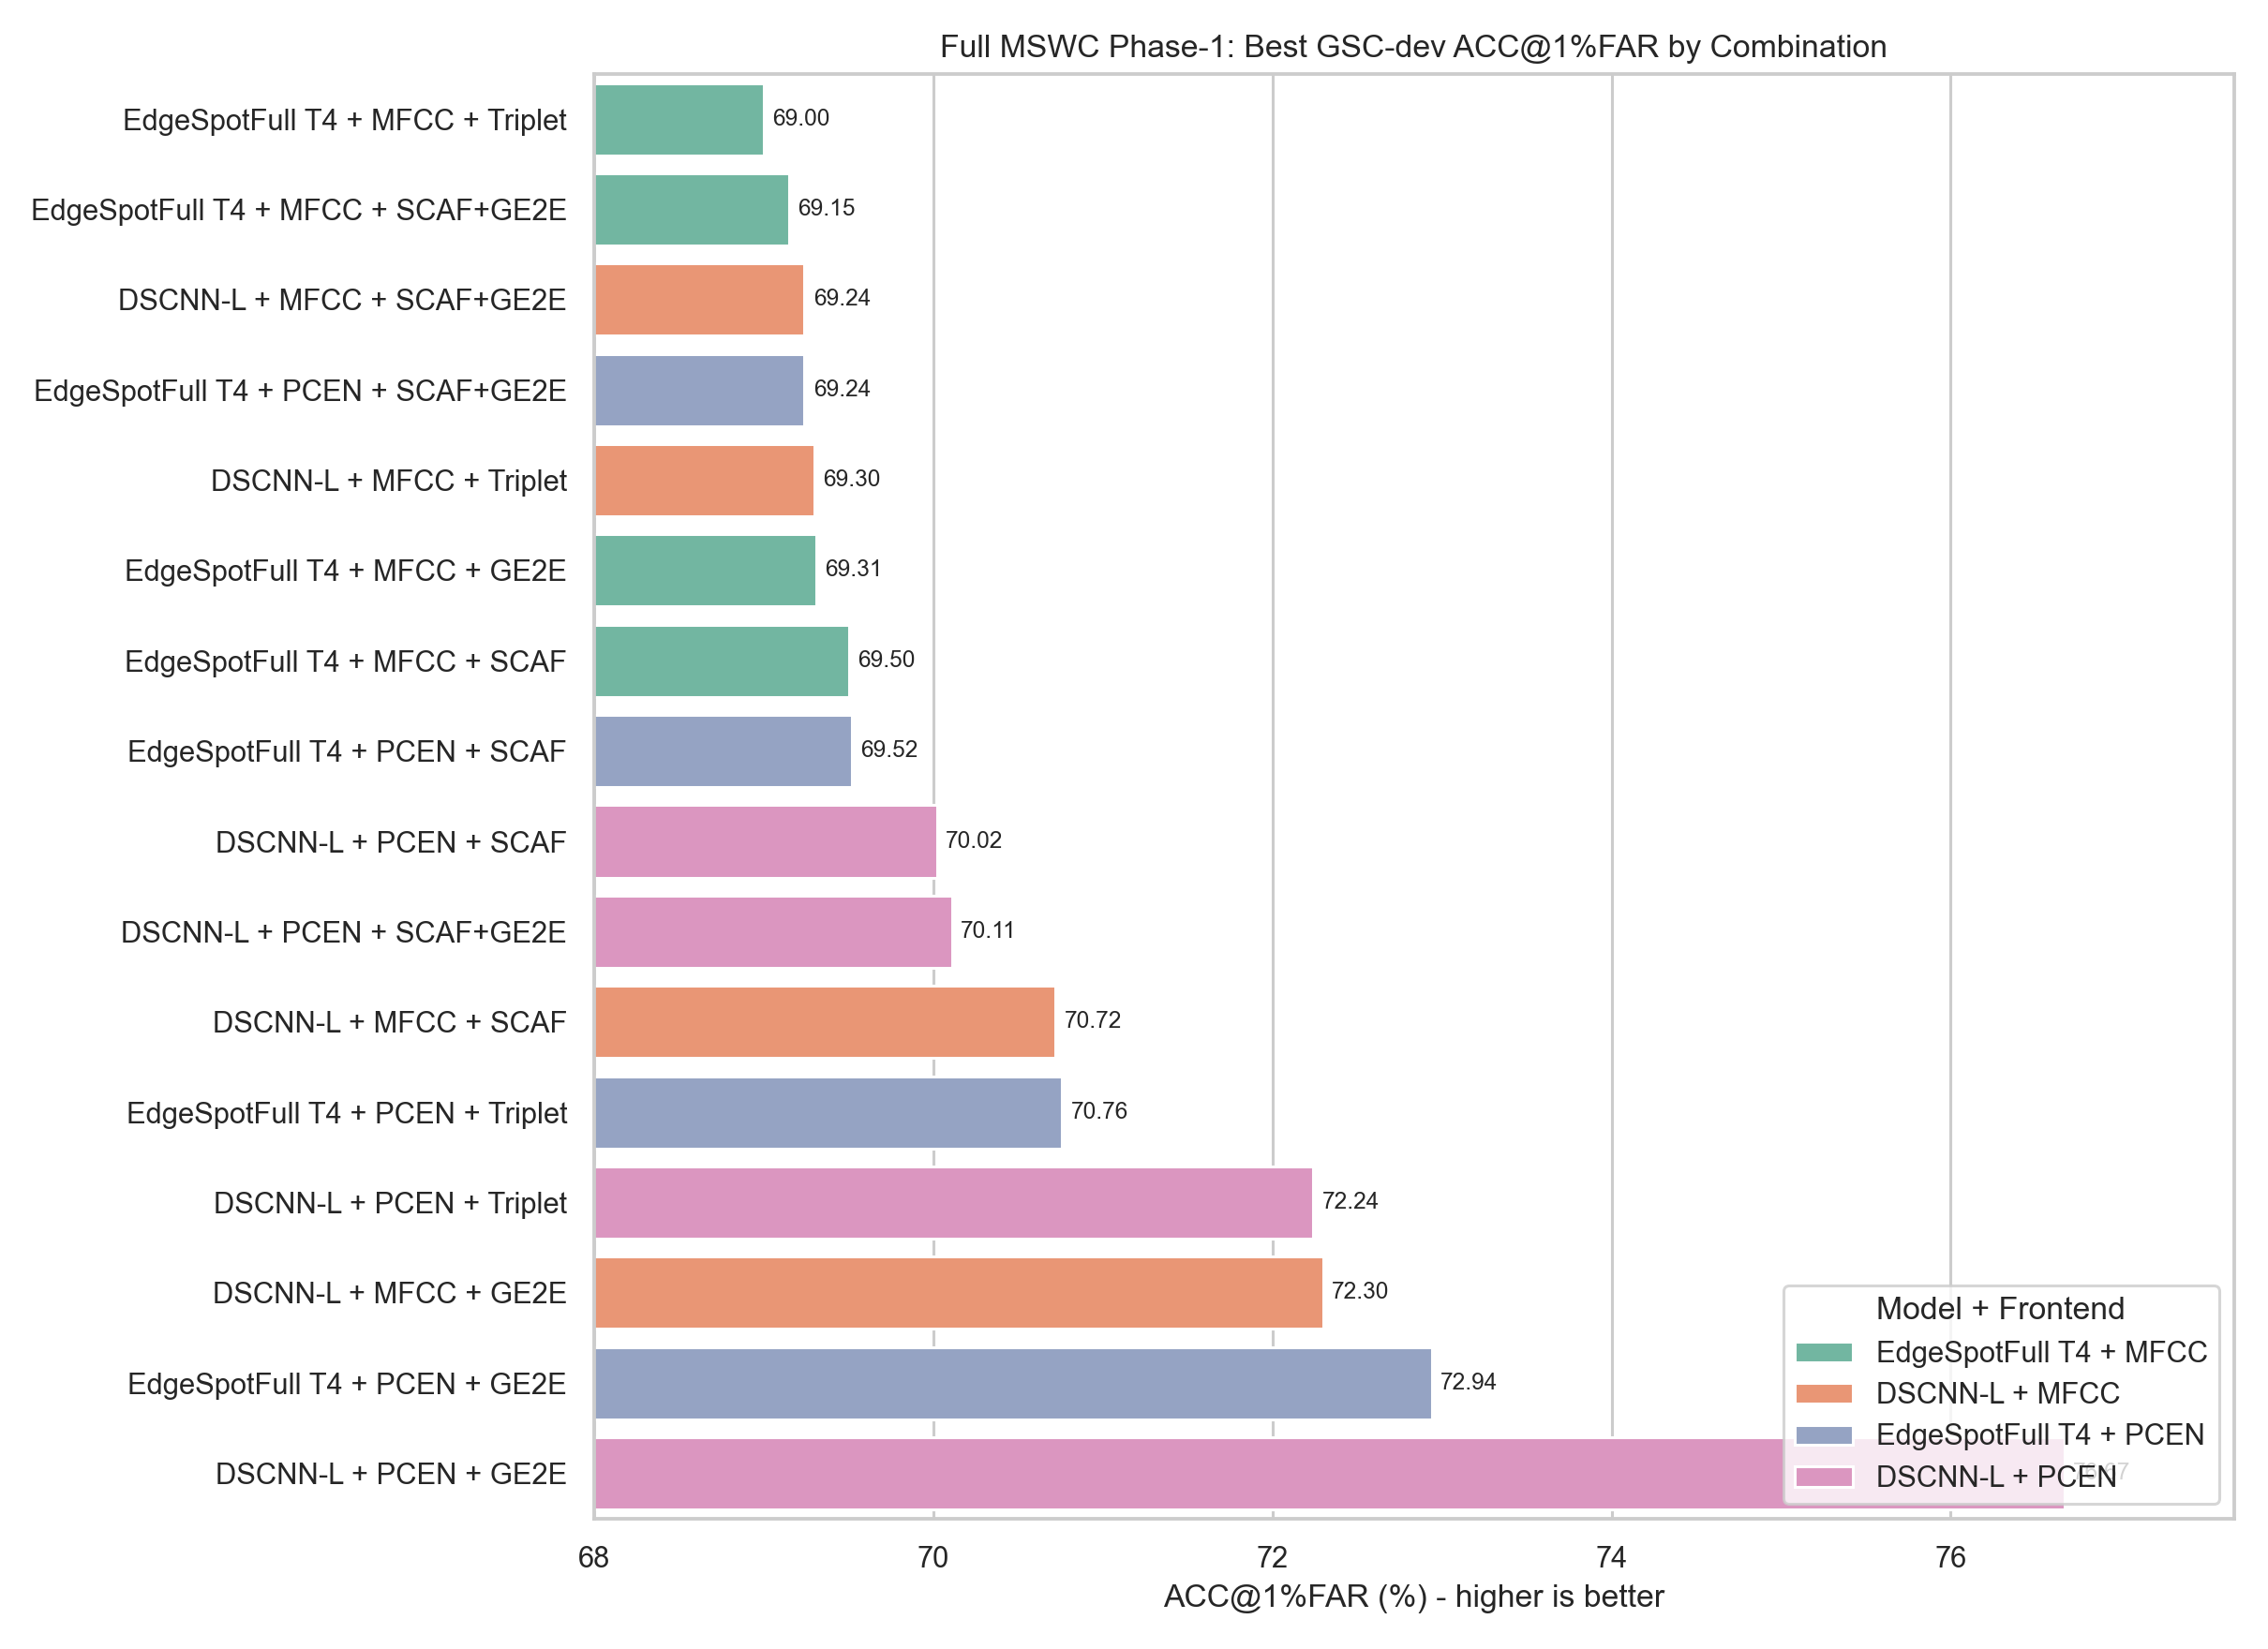
\includegraphics[width=0.96\linewidth]{res_ranked_bar.png}
\caption{Các cấu hình xếp hạng theo GSC ACC@1\%FAR (sàng lọc giai đoạn 1 trên
MSWC đầy đủ). Pipeline PCEN$+$GE2E dẫn đầu; màu sắc mã hóa backbone$\times$
đặc trưng. \emph{Hình kết quả từ dự án.}}
\label{fig:ranked}
\end{figure}

\paragraph{Lưu ý về cách đọc bảng sàng lọc.} \Cref{tab:matrix} là một lần chạy
\emph{sàng lọc} với ngân sách huấn luyện cố định, đồng nhất cho cả 16 cấu hình, nên
mục đích của nó là \emph{so sánh tương đối} giữa các trục thiết kế chứ không phải
đo đỉnh tuyệt đối. Vì vậy giá trị tuyệt đối ở đây thấp hơn một cách hệ thống so với
các lần chạy chuyên biệt dài hơn (ep300, chọn checkpoint theo chỉ số tổng hợp) được
tổng hợp ở \Cref{tab:final}: ví dụ DSCNN-L$+$PCEN$+$GE2E đạt $82{,}34$ ở bảng sàng
lọc nhưng $86{,}36$ ($+4{,}02$ điểm) khi được huấn luyện đầy đủ. Kết luận về thứ
hạng giữa các trục là nhất quán giữa hai chế độ.

\paragraph{Delta hiệu ứng cặp.}
Cô lập từng trục (\Cref{tab:deltas}, \Cref{fig:deltas}) cho thấy hai lợi thế ổn
định. PCEN cải thiện mọi backbone --- ấn tượng nhất là bộ mã hóa cạnh ($+9{,}22$
ACC, $+21{,}86$ F1) --- và GE2E nhất quán vượt triplet. Bộ trích xuất đặc trưng vì
vậy mang gánh nặng biểu diễn nhiều hơn theo tỷ lệ khi backbone nhỏ.

\begin{table}[H]
\centering
\caption{Delta hiệu ứng cặp (điểm phần trăm), MSWC toàn từ vựng,
GSC test100 @ 1\% FAR. Dương nghĩa là tùy chọn đầu tiên tốt hơn.}
\label{tab:deltas}
\small
\begin{tabular}{l r r r}
\toprule
\textbf{So sánh (các trục khác cố định)} & $\Delta\acc_{1\%}$ & $\Delta\auc$ & $\Delta$F1\\
\midrule
PCEN $-$ MFCC \;(DSCNN, GE2E)    & +5{,}26 & +5{,}96  & +9{,}25 \\
PCEN $-$ MFCC \;(Edge, GE2E)     & +9{,}22 & +21{,}93 & +21{,}86 \\
GE2E $-$ Triplet \;(DSCNN, PCEN) & +2{,}36 & +1{,}77  & +3{,}61 \\
DSCNN $-$ Edge \;(PCEN, GE2E)    & +2{,}36 & +5{,}19  & +7{,}07 \\
\bottomrule
\end{tabular}
\end{table}

\paragraph{Ý nghĩa thực tế.} Hai lựa chọn ``rẻ'' về chi phí --- đổi bộ trích xuất
sang PCEN và đổi hàm mục tiêu sang GE2E --- mang lại phần lớn lợi ích mà không làm
tăng kích thước mô hình. Với người làm sản phẩm, điều này nghĩa là một thiết bị
dùng bộ mã hóa cạnh nhỏ vẫn có thể tăng đáng kể độ tin cậy chỉ bằng cách thay khối
tiền xử lý và cách huấn luyện, thay vì phải dùng mô hình lớn hơn và tốn pin hơn.

\begin{figure}[H]
\centering
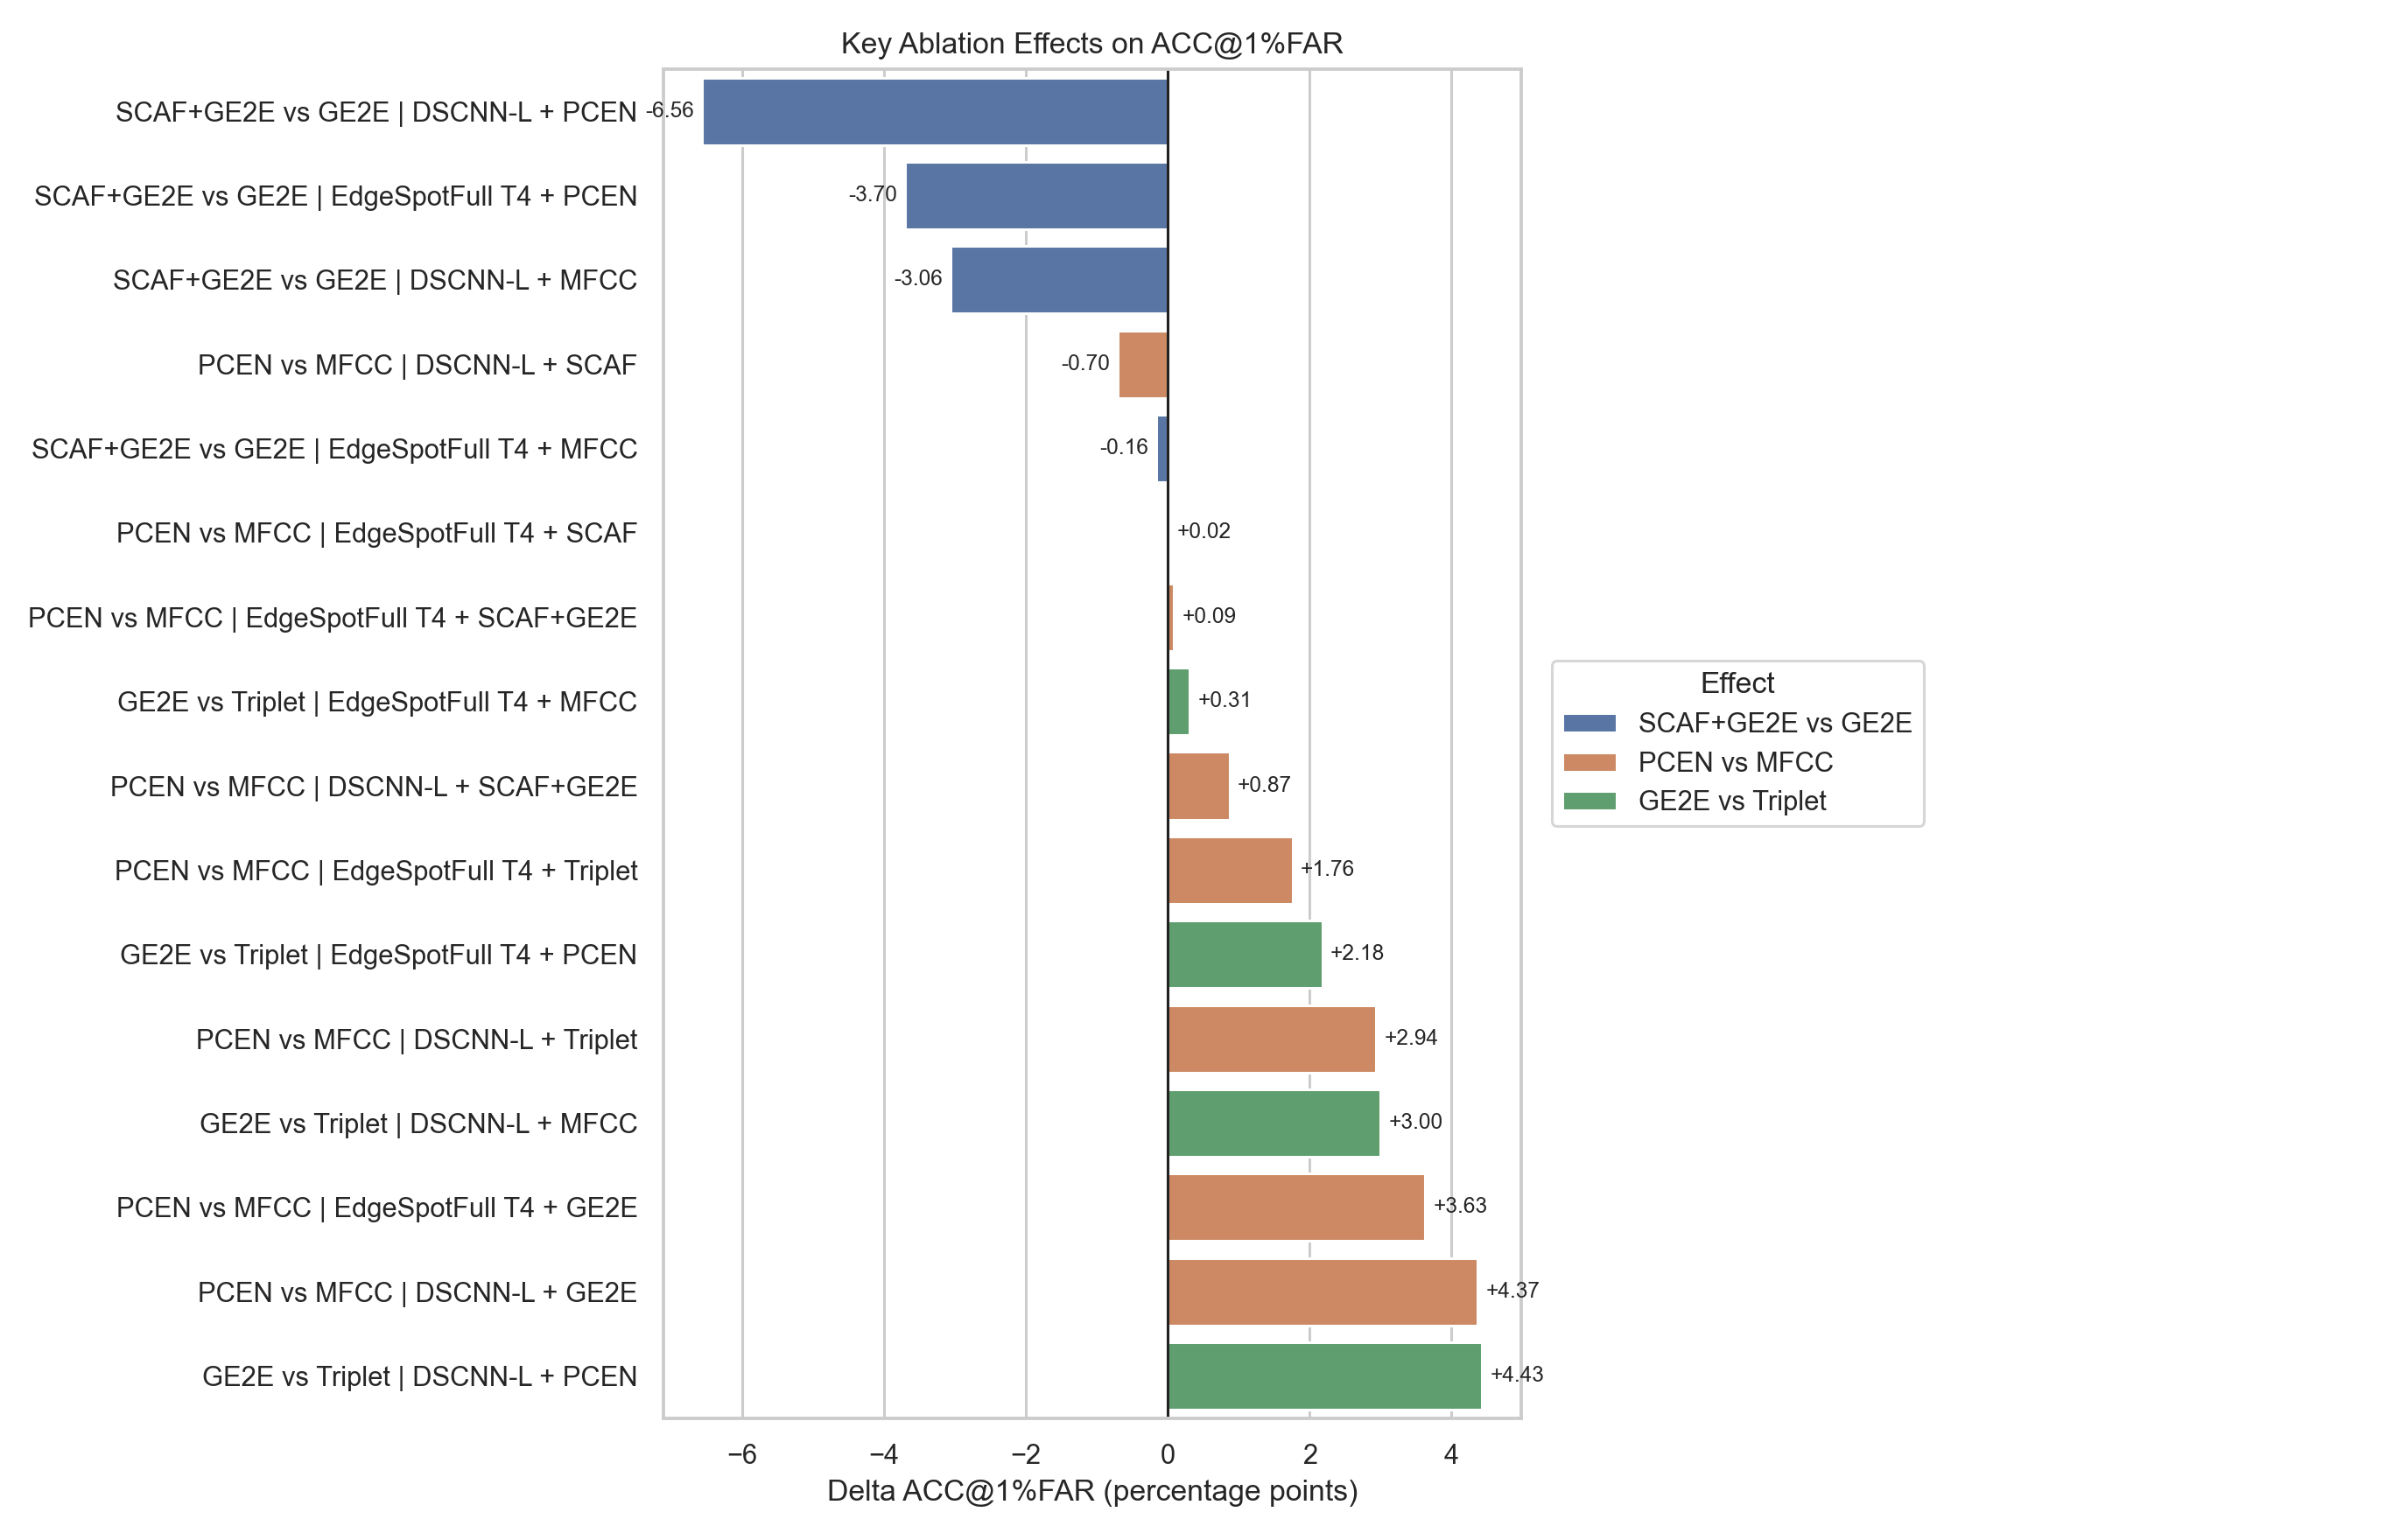
\includegraphics[width=0.92\linewidth]{res_effect_deltas.png}
\caption{Các delta hiệu ứng cặp chính. PCEN và GE2E là hai cải tiến nhất quán qua
các backbone. \emph{Hình kết quả từ dự án.}}
\label{fig:deltas}
\end{figure}

\section{Q2: Quy Mô --- Bão Hòa và Sụp Đổ SCAF}\label{sec:res-q2}

\begin{table}[H]
\centering
\caption{Quét quy mô dữ liệu (PCEN$+$GE2E), GSC test100, ACC tại 5\% FAR. Mỗi cap
là một lần chạy huấn luyện riêng (ngân sách huấn luyện khác nhau giữa các cap); các
dòng cap-$\{20,50,220\}$ kèm std qua 100 lần chạy đánh giá, riêng dòng cap-620 lấy
từ một lần chạy bão hòa mà std từng-lần-chạy không được ghi nhận.}
\label{tab:scale}
\small
\begin{tabular}{l c r r r r}
\toprule
\textbf{Bộ mã hóa} & \textbf{Giới hạn} & \acc$_{5\%}$ & \auc & \eer & F1\\
\midrule
\multirow{4}{*}{DSCNN-L}
 & 20  & 86{,}05$\pm$0{,}66 & 91{,}57$\pm$0{,}58 & 16{,}25$\pm$0{,}86 & 75{,}90$\pm$1{,}16 \\
 & 50  & 84{,}68$\pm$0{,}70 & 90{,}45$\pm$0{,}68 & 17{,}42$\pm$1{,}08 & 74{,}34$\pm$1{,}43 \\
 & 220 & 88{,}23$\pm$0{,}68 & 93{,}87$\pm$0{,}47 & 12{,}78$\pm$0{,}80 & 80{,}67$\pm$1{,}12 \\
 & 620 & \best{88{,}56} & \best{94{,}04} & \best{12{,}53} & \best{81{,}02} \\
\midrule
\multirow{4}{*}{EdgeSpot}
 & 20  & 83{,}06$\pm$0{,}82 & 87{,}22$\pm$0{,}75 & 20{,}40$\pm$1{,}01 & 70{,}46$\pm$1{,}30 \\
 & 50  & 82{,}24$\pm$0{,}74 & 87{,}74$\pm$0{,}66 & 20{,}19$\pm$0{,}90 & 70{,}73$\pm$1{,}16 \\
 & 220 & \best{86{,}03}$\pm$0{,}70 & 91{,}31$\pm$0{,}62 & 16{,}47$\pm$0{,}78 & 75{,}61$\pm$1{,}06 \\
 & 620 & 86{,}01 & \best{91{,}34} & 16{,}64 & 75{,}38 \\
\bottomrule
\end{tabular}
\end{table}

\paragraph{Độ chính xác bão hòa gần 2\,M clip.}
\Cref{fig:saturation} và \Cref{tab:scale} quét giới hạn mỗi từ cho frontend/loss
tốt nhất (PCEN$+$GE2E). Có bước nhảy lớn giữa cap-50 và cap-220 ($+3{,}55$ ACC
cho DSCNN, $+3{,}79$ cho EdgeSpot tại 5\% FAR) và vùng phẳng từ cap-220 đến
cap-620 ($+0{,}33$/$-0{,}02$). Độ chính xác thực sự bão hòa dữ liệu tại
$\sim$2\,M clip huấn luyện.

\begin{figure}[H]
\centering
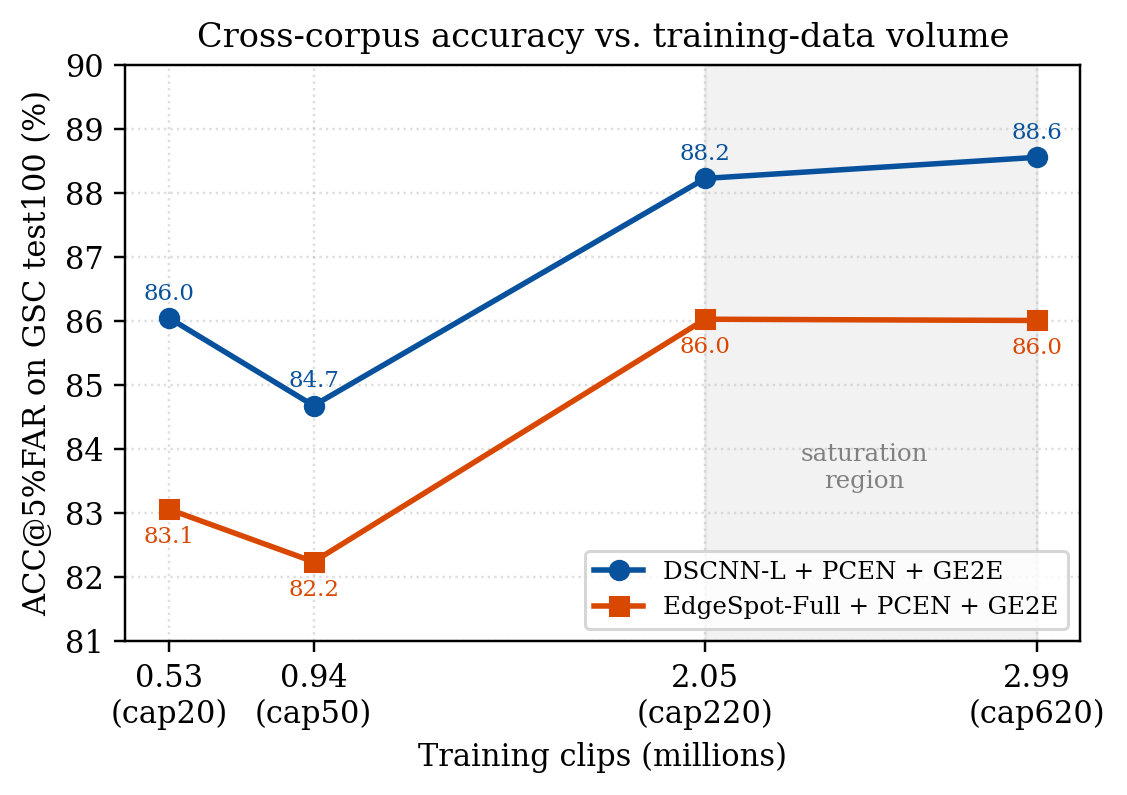
\includegraphics[width=0.80\linewidth]{fig_data_saturation.png}
\caption{Độ chính xác chéo kho ngữ liệu vs.\ khối lượng dữ liệu huấn luyện (giới
hạn mỗi từ). Hiệu suất bão hòa gần $\sim$2\,M clip (vùng tô màu).
\emph{Tạo từ kết quả dự án.}}
\label{fig:saturation}
\end{figure}

\paragraph{Sụp đổ SCAF tại 37k lớp.}
Kết quả ấn tượng nhất của nghiên cứu quy mô là thất bại định tính. Trên micro-set
31 lớp và phân chia Top-500 $\sim$500 lớp, SCAF và SCAF$+$GE2E rất xuất sắc (AUC
$\approx 95$). Tuy nhiên, trên từ vựng đầy đủ 37.387 lớp với trọng số SCAF mặc
định 1{,}0, huấn luyện sụp đổ từ epoch~2: AUC kiểm định ghim tại 0{,}5000 và độ
chính xác GE2E trong phép học giảm xuống $\approx 0{,}033$ (ngẫu nhiên). Các chỉ số
GSC chéo kho ngữ liệu cũng suy biến tương ứng (\Cref{fig:scafcollapse}): AUC 50,
F1 0, $\frr{=}100\%$, keyword ACC 9{,}09\% ($={}$$1/11$ lớp), trong khi ACC@1\%FAR
tập mở vẫn ở mức \emph{gây hiểu nhầm} 69{,}4\% --- một hiện tượng từ-chối-tất-cả
mà AUC, F1 và FRR lập tức phơi bày.
Cơ chế là mất cân bằng gradient: thang logit ArcFace ($s{=}30$) nhân qua
$\sim$3{,}7$\times$10$^4$ lớp tạo ra gradient phân loại áp đảo các số hạng
centroid/cosine. Các biện pháp khắc phục thực tế: (i) giảm trọng số SCAF xuống
$\sim$5$\times$10$^{-5}$, (ii) làm ấm biên/thang, hoặc (iii) bỏ số hạng phân loại
và dùng GE2E hoặc KD.

\begin{figure}[H]
\centering
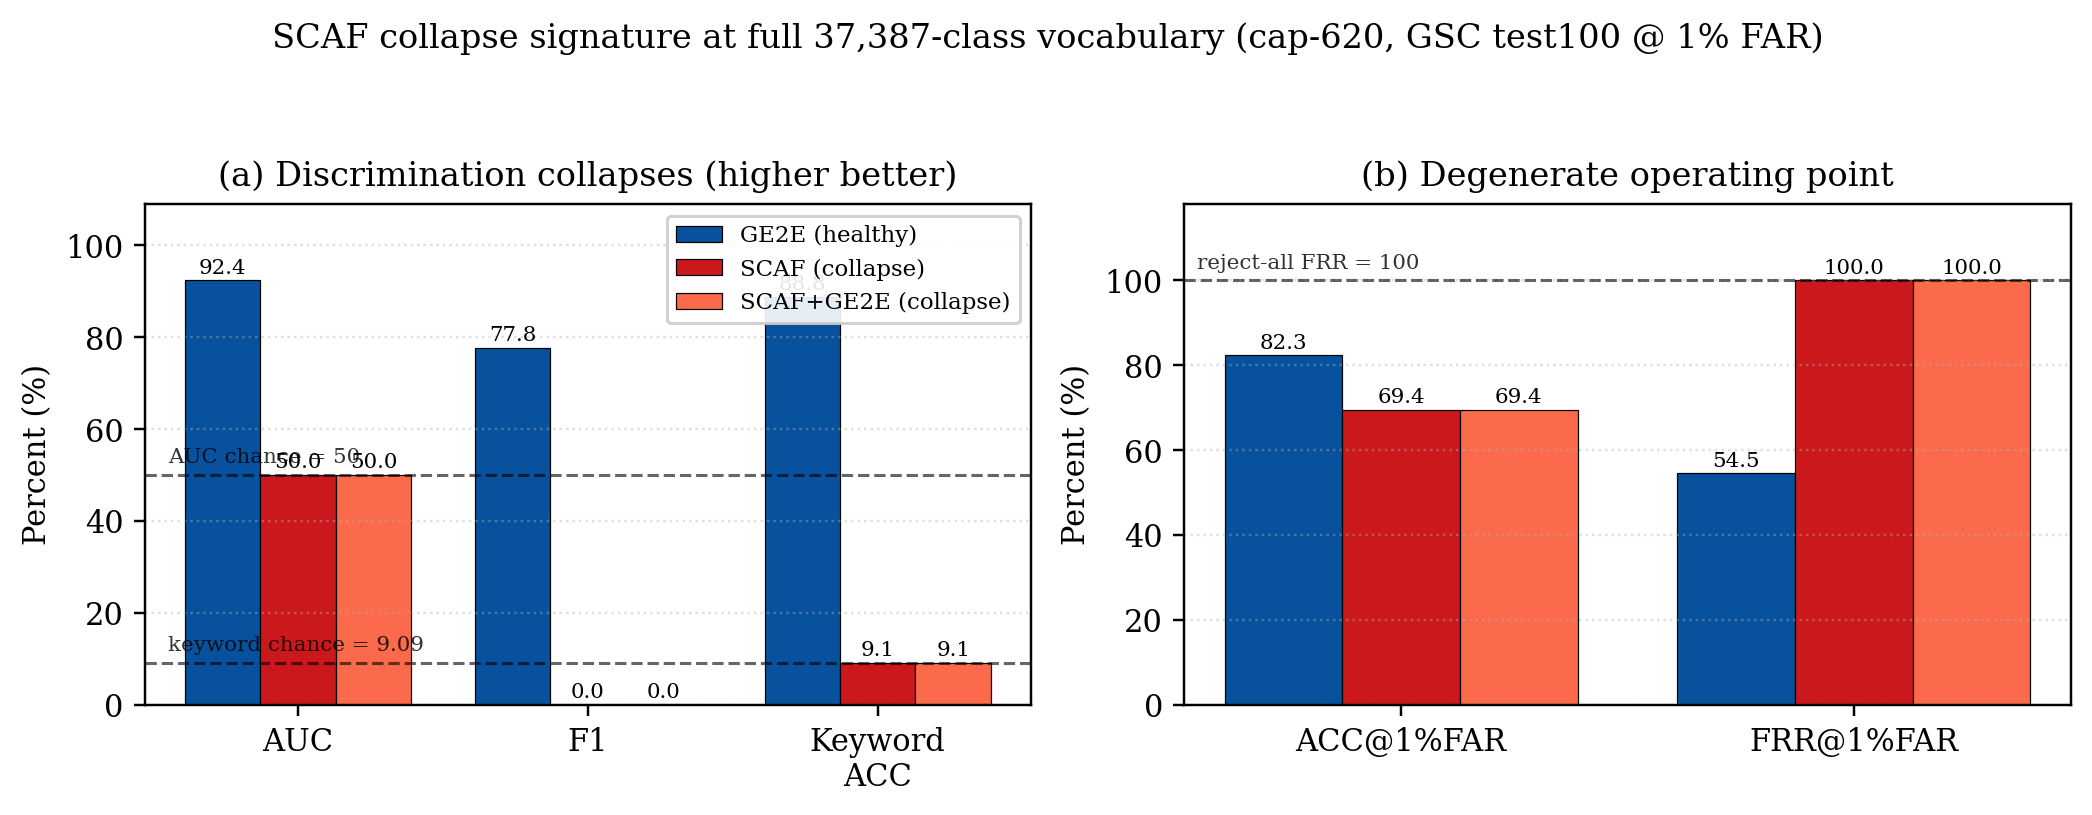
\includegraphics[width=0.92\linewidth]{scaf_collapse.png}
\caption{\NEW{Dấu hiệu sụp đổ của SCAF và SCAF$+$GE2E ở từ vựng đầy đủ 37.387 lớp
(cap-620, GSC test100 @ 1\% FAR), đối chiếu với cấu hình lành mạnh
DSCNN-L$+$PCEN$+$GE2E. (a) Các chỉ số phân biệt rơi đáy: AUC về mức ngẫu nhiên (50),
F1 về 0 và keyword ACC về 9{,}09\% ($={}$$1/11$). (b) Điểm hoạt động suy biến: các
run sụp đổ từ chối tất cả ($\frr{=}100\%$), nhưng ACC@1\%FAR tập mở vẫn ở mức gây
hiểu nhầm $\sim$69\% nhờ số lượng mẫu âm lớn. Mọi giá trị là chỉ số cuối thật của
cap-620 (cùng nguồn với \Cref{tab:matrix}).}}
\label{fig:scafcollapse}
\end{figure}

\paragraph{Ý nghĩa thực tế.} Hai phát hiện ở Q2 có hệ quả vận hành rõ ràng. Bão hòa
gần $\sim$2\,M clip nghĩa là sau một ngưỡng nhất định, việc thu thập thêm dữ liệu
cho mỗi từ gần như không cải thiện độ chính xác --- nên ngân sách thu dữ liệu nên
ưu tiên \emph{đa dạng từ và điều kiện ghi âm} hơn là thêm clip cho cùng một từ. Sụp
đổ SCAF ở quy mô lớn là lời cảnh báo: một hàm mất mát xuất sắc ở quy mô nhỏ có thể
phá hỏng toàn bộ huấn luyện ở quy mô thật nếu không được điều chỉnh, nên cần kiểm
tra lại các lựa chọn thiết kế mỗi khi tăng quy mô thay vì giả định chúng vẫn đúng.

\section{Q3: Chưng Cất Đổi Kiến Thức Giáo Viên Lấy Dữ Liệu}\label{sec:res-q3}

\begin{table}[H]
\centering
\caption{Chưng cất kiến thức vs.\ GE2E (sinh viên EdgeSpot), GSC test100.
``n/a'' nghĩa là ACC@1\%FAR không được ghi nhận cho lần chạy cap-220 GE2E này (chỉ
có ACC@5\%FAR); so sánh ở cap-220 vì vậy dựa trên cột ACC@5\%FAR.}
\label{tab:kd}
\small
\begin{tabular}{l l r r r r}
\toprule
\textbf{Giới hạn} & \textbf{Loss} & \acc$_{1\%}$ & \acc$_{5\%}$ & \eer & F1\\
\midrule
50  & GE2E & 77{,}14 & 82{,}24 & 20{,}19 & 70{,}73 \\
\rowcolor{blue!7}
50  & KD   & \best{80{,}74} & \best{85{,}82} & \best{15{,}41} & \best{77{,}04} \\
220 & GE2E & n/a & 86{,}03 & 16{,}47 & 75{,}61 \\
220 & KD   & 80{,}82 & 85{,}90 & 15{,}36 & 77{,}10 \\
\bottomrule
\end{tabular}
\end{table}

\Cref{tab:kd} chưng cất mô hình giáo viên Wav2Vec\,2.0 đóng băng vào sinh viên
EdgeSpot nhỏ gọn. Ở cap-50, KD cải thiện mọi chỉ số so với GE2E ($+3{,}60$
ACC@1\%FAR, $-4{,}78$ EER, $+6{,}31$ F1) và, đáng chú ý, KD ở cap-50 khớp GE2E
ở cap-220 --- cùng độ chính xác với khoảng một nửa clip huấn luyện. KD cũng bão
hòa sớm (cap-50$\to$cap-220 gần như phẳng), cho thấy mô hình giáo viên tiêm hầu
hết thiên kiến quy nạp hữu ích từ dữ liệu hạn chế.

\paragraph{Ý nghĩa thực tế.} Kết quả này có giá trị khi dữ liệu khan hiếm: một
mô hình giáo viên mạnh có thể bù cho việc thiếu dữ liệu, giúp đạt cùng độ chính xác
với khoảng một nửa số clip. Với nhóm phát triển không có sẵn kho dữ liệu lớn cho
từng từ, chưng cất là cách thực tế để rút ngắn chi phí thu thập dữ liệu mà vẫn giữ
mô hình triển khai nhỏ gọn.

\section{Q4: Các Hệ Thống Triển Khai Tốt Nhất}\label{sec:res-q4}

\begin{table}[H]
\centering
\caption{Tổng hợp hệ thống tốt nhất theo chế độ dữ liệu (GSC test100,
EdgeSpot-exact 10 mẫu, 100 lần chạy). ``sụp.''$=$ sụp đổ suy biến; ``n/a''$=$
ACC@1\%FAR không được ghi nhận cho lần chạy đó. Để bảng dễ đọc, độ lệch chuẩn
($\pm$) của ba cấu hình chủ lực được nêu trong văn bản ở trên (cỡ $\pm0{,}4$ đến
$\pm1{,}3$ điểm); các dòng còn lại là một lần chạy huấn luyện mỗi chế độ.}
\label{tab:final}
\scriptsize
\setlength{\tabcolsep}{3pt}
\begin{tabular}{l l l c r r r r r r}
\toprule
\textbf{Chế độ} & \textbf{Bộ mã hóa} & \textbf{Loss} & \textbf{Tham số} &
\acc$_{1\%}$ & \acc$_{5\%}$ & \auc & \eer & F1 & KW\\
\midrule
Micro (31)    & EdgeSpot & SCAF+GE2E      & 0{,}131M & 84{,}61 & 86{,}12 & 95{,}61 & 11{,}54 & 82{,}41 & 77{,}66 \\
Top-500       & EdgeSpot & SCAF+GE2E\,ep13& 0{,}131M & 85{,}62 & 88{,}79 & 95{,}34 & 11{,}51 & 82{,}45 & 90{,}44 \\
Top-500       & DSCNN-L  & GE2E           & 0{,}413M & 81{,}55 & 86{,}56 & 93{,}17 & 14{,}00 & 78{,}97 & 88{,}62 \\
Full cap20    & DSCNN-L  & GE2E           & 0{,}413M & 82{,}10 & 86{,}05 & 91{,}57 & 16{,}25 & 75{,}90 & 88{,}90 \\
Full cap220   & DSCNN-L  & GE2E           & 0{,}413M & n/a & 88{,}23 & 93{,}87 & 12{,}78 & 80{,}67 & 89{,}82 \\
\rowcolor{blue!7}
Full cap620   & DSCNN-L  & GE2E\,ep300    & 0{,}413M & \best{86{,}36} & \best{89{,}93} & \best{95{,}21} & \best{11{,}32} & \best{82{,}73} & \best{92{,}92} \\
Full cap620   & EdgeSpot & GE2E\,ep300    & 0{,}131M & 82{,}87 & 86{,}76 & 92{,}41 & 14{,}82 & 77{,}85 & 87{,}29 \\
Full cap50    & EdgeSpot & KD             & 0{,}131M & 80{,}74 & 85{,}82 & 91{,}19 & 15{,}41 & 77{,}04 & 87{,}95 \\
Full cap220   & EdgeSpot & SCAF+GE2E      & 0{,}131M & sụp. & sụp. & 50{,}00 & 50{,}00 & sụp. & 9{,}09 \\
\bottomrule
\end{tabular}
\end{table}

\Cref{tab:final} tổng hợp các cấu hình mạnh nhất theo từng chế độ dữ liệu. Khác với
bảng sàng lọc ngân sách cố định ở \Cref{sec:res-q1}, các dòng cap-620 ``ep300'' tại
đây là những lần chạy chuyên biệt được huấn luyện đầy đủ và chọn checkpoint theo chỉ
số tổng hợp trên GSC-dev, nên đạt đỉnh tuyệt đối cao hơn.
Ba điểm nổi bật:
\begin{itemize}[leftmargin=1.3em,itemsep=2pt]
\item \textbf{Tốt nhất tổng thể:} DSCNN-L$+$PCEN$+$GE2E (cap-620) đạt
\best{$86{,}36\pm1{,}29$} ACC@1\%FAR và $89{,}93\pm0{,}65$ tại 5\% FAR, với AUC
95{,}21, EER 11{,}32, F1 82{,}73, keyword ACC 92{,}92\%.
\item \textbf{Tốt nhất nhỏ gọn:} EdgeSpot-Full$+$PCEN$+$GE2E (cap-620) đạt
$82{,}87\pm1{,}22$ ACC@1\%FAR với 0{,}131\,M tham số --- cách hệ thống tốt nhất
$\sim$3{,}5 điểm nhưng nhỏ hơn ba lần.
\item \textbf{Tốt nhất từ vựng nhỏ:} trên phân chia Top-500, kết hợp
EdgeSpot$+$PCEN$+$SCAF$+$GE2E là mô hình nhỏ gọn mạnh nhất ($85{,}62\pm1{,}04$
ACC@1\%FAR, AUC 95{,}34), xác nhận rằng kết hợp lai xuất sắc \emph{khi số lớp
đủ nhỏ để không kích hoạt sụp đổ}.
\end{itemize}

\Cref{fig:res-q4} tóm tắt câu chuyện của chương bằng hai góc nhìn bổ trợ: đường
cong DET cho thấy hệ thống tốt nhất giữ tỉ lệ bỏ sót thấp trên dải tỉ lệ báo nhầm
rộng, còn bản đồ nhiệt xác nhận PCEN$+$GE2E là vùng sáng nhất bất kể backbone.

\begin{figure}[H]
\centering
\begin{subfigure}{0.49\linewidth}
  \centering
  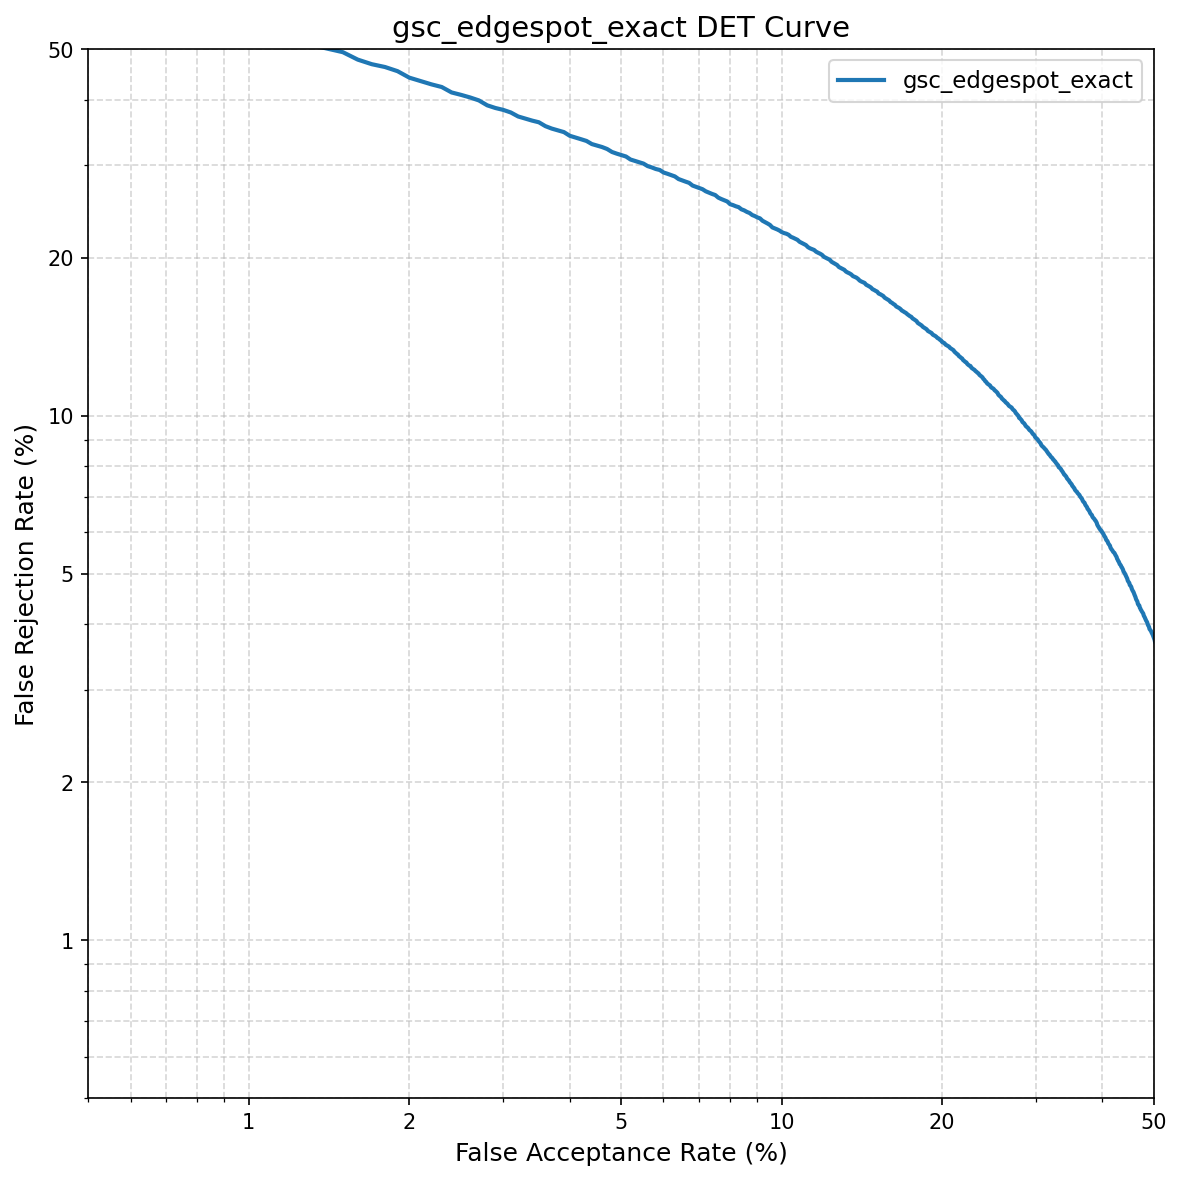
\includegraphics[width=\linewidth]{res_det_dscnn.png}
  \caption{Đường cong DET (DSCNN-L$+$PCEN$+$GE2E).}
  \label{fig:detcurve}
\end{subfigure}\hfill
\begin{subfigure}{0.49\linewidth}
  \centering
  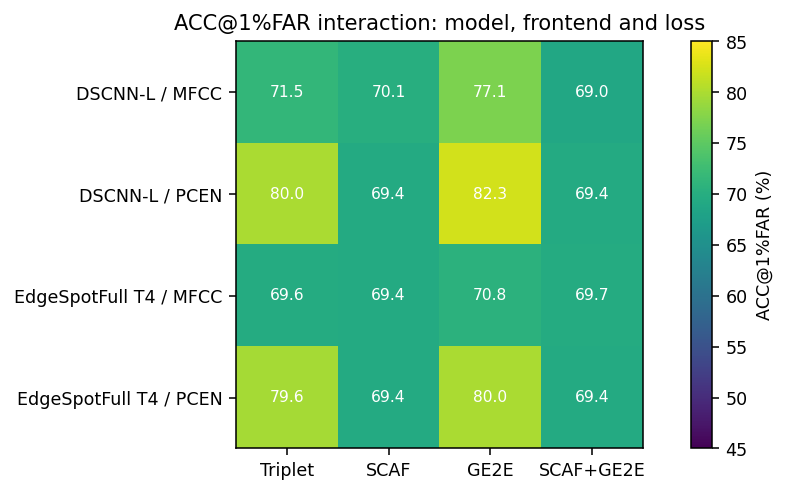
\includegraphics[width=\linewidth]{res_cap620_heatmap.png}
  \caption{Bản đồ nhiệt ACC@1\%FAR (cap-620).}
  \label{fig:heatmap}
\end{subfigure}
\caption{Các góc nhìn về điểm hoạt động. (a) Đường cong đánh đổi lỗi phát hiện
của hệ thống tổng thể tốt nhất; (b) bản đồ nhiệt độ chính xác ACC@1\%FAR qua các
cấu hình cap-620, cho thấy ô PCEN$+$GE2E sáng nhất ở cả hai backbone.
\emph{Hình kết quả từ dự án.}}
\label{fig:res-q4}
\end{figure}

\paragraph{Ý nghĩa thực tế.} Bảng tổng hợp cho thấy người triển khai có hai lựa
chọn rõ ràng tùy ràng buộc phần cứng: nếu ưu tiên độ chính xác và còn dư tài
nguyên thì dùng DSCNN-L$+$PCEN$+$GE2E; nếu bị giới hạn bộ nhớ/pin thì EdgeSpot-Full
nhỏ hơn ba lần chỉ kém khoảng 3,5 điểm --- một mức đánh đổi chấp nhận được cho thiết
bị biên. Quan trọng hơn, cùng một bộ mã hóa phục vụ được vô số bộ từ khóa hạ nguồn
mà không cần huấn luyện lại, nên chi phí một lần này được khấu hao trên mọi ứng dụng.

\section{Suy Luận Trên Audio Dài}\label{sec:res-inference}
\reviewnote{Mục mới, tương tự mục ``Kết Quả Suy Luận'' của đồ án mẫu.
\Cref{fig:longinfer} được tạo bằng cách thực sự chạy mô hình đã huấn luyện trên
bản ghi đa từ thật.}

Để xác minh hệ thống hoạt động đầu cuối --- không chỉ trên clip kiểm tra riêng lẻ
--- chúng tôi đăng ký prototype cho 17 từ khóa (10 mẫu mỗi từ từ GSC) và chạy
suy luận prototype gần nhất trên bản ghi liên tục đa từ thật.

\begin{figure}[H]
\centering
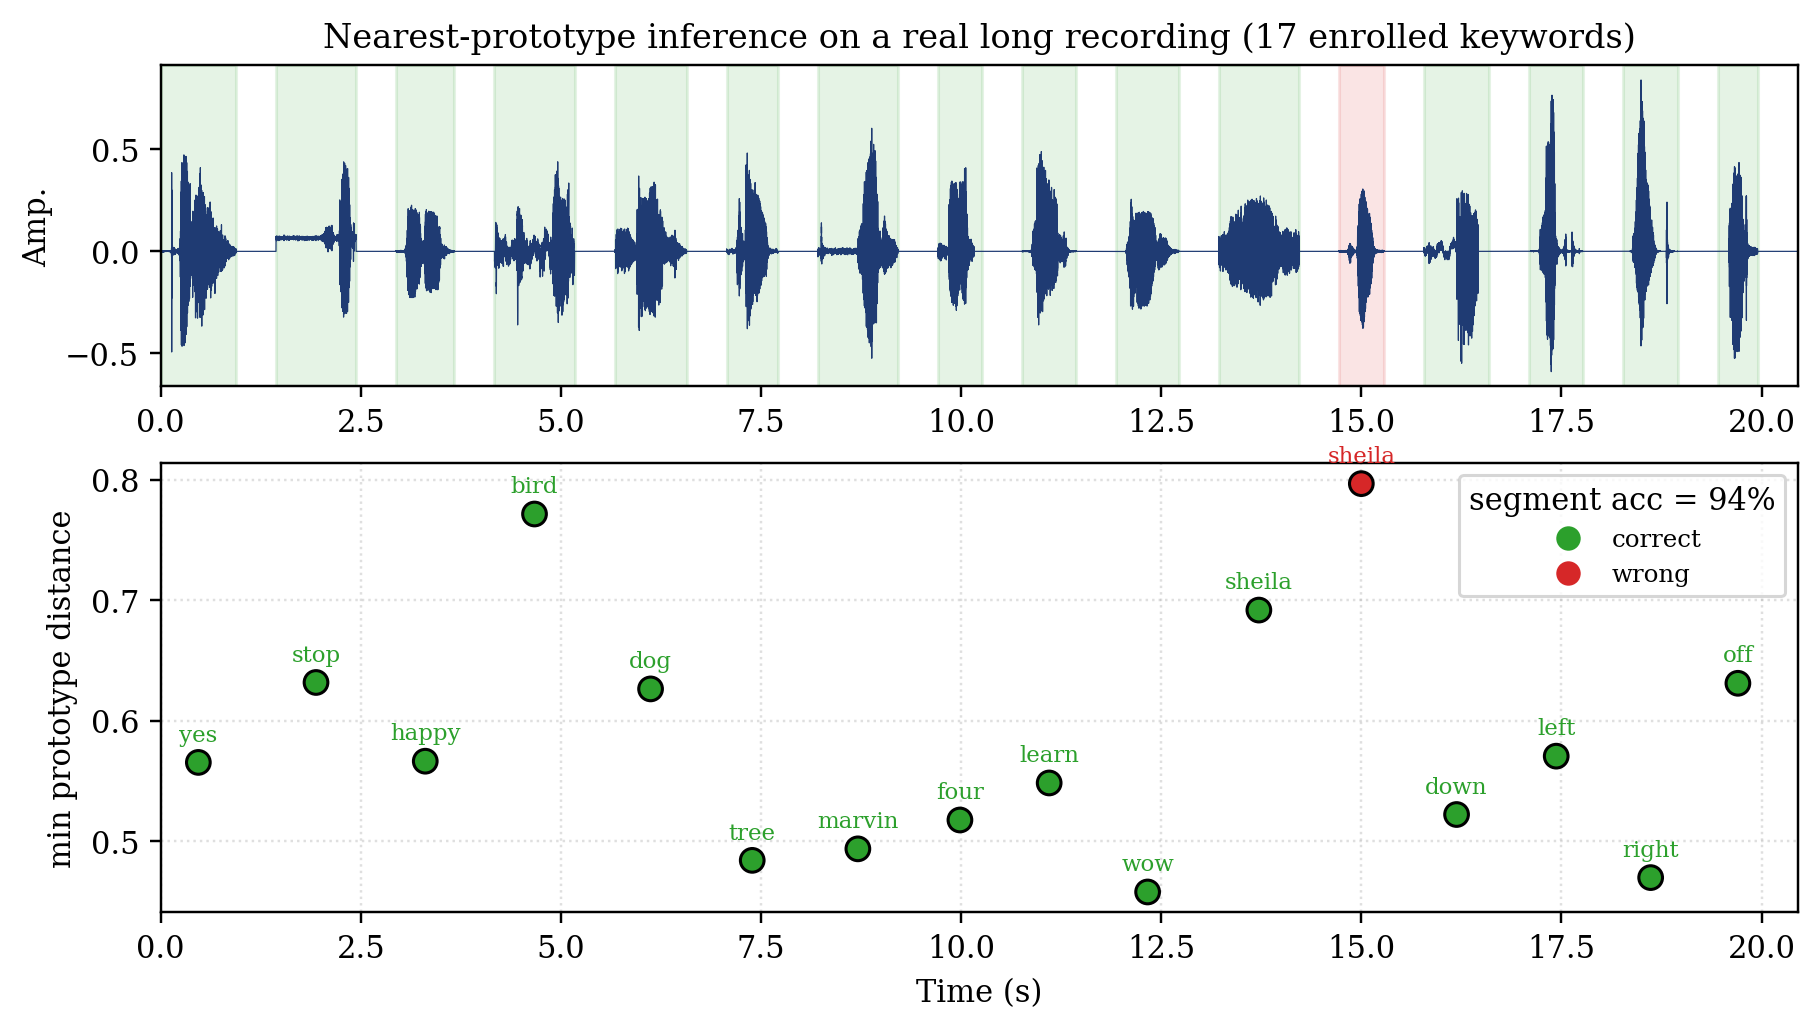
\includegraphics[width=0.98\linewidth]{fig_long_inference.png}
\caption{\NEW{Suy luận prototype gần nhất trên bản ghi dài thật. Trên: dạng sóng
với tô màu đúng (xanh)/sai (đỏ) mỗi đoạn. Dưới: khoảng cách prototype tối thiểu
và từ khóa dự đoán mỗi đoạn.}}
\label{fig:longinfer}
\end{figure}

\Cref{fig:longinfer} chồng lên dạng sóng từ khóa dự đoán và khoảng cách prototype của nó cho 16 đoạn
nói đầu tiên. Mô hình nhận dạng đúng $15/16$ đoạn ($\approx$94\%); lỗi duy nhất
(``sheila'', tên dài, hiếm) cũng có khoảng cách prototype lớn nhất --- đúng là tín
hiệu mà ngưỡng tập mở dùng để đánh dấu phát hiện độ tin thấp.

%==============================================================================
\chapter{Kết Luận}\label{ch:conclusion}
\reviewnote{Chương mới ($\sim$2 trang): hiện trạng, điểm mạnh, điểm yếu, hướng
phát triển tương lai.}

Chương này khép lại đồ án bằng cách nhìn lại toàn bộ hành trình: từ bài toán đặt ra
ở \Cref{ch:intro}, phương pháp ở \Cref{ch:method}, đến bằng chứng thực nghiệm ở
\Cref{ch:results}. Chúng tôi tóm tắt hiện trạng hệ thống, nêu rõ điểm mạnh và điểm
yếu một cách trung thực, rồi vạch ra các hướng phát triển tiếp theo bắt nguồn trực
tiếp từ những hạn chế đã quan sát được.

\section{Hiện Trạng}\label{sec:status}

Đồ án này nhằm xây dựng hệ thống nhận dạng từ khóa thoát khỏi hai giới hạn cấu
trúc của các engine từ đánh thức cổ điển --- từ vựng đóng băng và không thể từ
chối --- đồng thời hiểu được, chứ không chỉ đơn thuần báo cáo, điều gì khiến hệ
thống như vậy hoạt động khi từ vựng huấn luyện tăng. Chúng tôi đã cung cấp một
pipeline hoàn chỉnh, có thể tái tạo, ít phụ thuộc: hai bộ mã hóa nhỏ gọn (DSCNN-L
$\approx$0{,}41\,M và EdgeSpot-Full $\approx$0{,}13\,M tham số), ba bộ trích xuất
đặc trưng, bốn hàm mục tiêu học độ đo, bốn đầu từ chối tập mở, engine phát trực
tuyến CPU và bản demo web offline. Mọi hệ thống được huấn luyện trên MSWC tiếng
Anh và đánh giá chéo kho ngữ liệu trên GSC v2 theo một giao thức EdgeSpot-exact
10 mẫu nghiêm ngặt với 100 lần chạy ngẫu nhiên.

Kết quả chính là nhận dạng từ khóa ít mẫu tập mở khả thi và thậm chí mạnh ở quy
mô từ vựng thật: huấn luyện một lần trên $37{.}387$ từ, cấu hình tốt nhất
(DSCNN-L $+$ PCEN $+$ GE2E) đạt $86{,}36\%$ độ chính xác tập mở tại 1\% FAR và
AUC $95{,}21$ trên kho ngữ liệu chưa từng được huấn luyện, trong khi mô hình nhỏ
hơn ba lần vẫn cách vài điểm. Người dùng có thể tự định nghĩa tập từ khóa tùy ý
từ mười ví dụ mỗi từ, không cần huấn luyện lại, và hệ thống có thể từ chối lời
nói không biết và tiếng im lặng.

\section{Điểm Mạnh và Điểm Yếu}\label{sec:goodbad}

\paragraph{Điều hoạt động tốt.} Ba phát hiện bền vững và có thể chuyển giao.
(1) Bộ trích xuất PCEN có thể học được là cải tiến đơn lẻ đáng tin cậy nhất, và
nó giúp bộ mã hóa nhỏ hơn nhiều nhất --- một đòn bẩy hữu ích chính xác khi ngân
sách tham số hạn chế nhất. (2) Hàm mục tiêu centroid GE2E, tối ưu hóa cùng tính
toán đăng ký-rồi-khớp dùng khi triển khai, nhất quán vượt cả triplet lẫn phân
loại cho tổng quát hóa tập mở. (3) Mô hình giáo viên Wav2Vec\,2.0 đóng băng chưng
cất với hàm mất mát cosine đơn giản cho phép mô hình nhỏ gọn đạt độ chính xác
ngang GE2E với khoảng một nửa dữ liệu.

\paragraph{Điểm yếu / những gì chúng tôi học được theo cách khó.} Kết quả phủ
định rõ ràng nhất là sụp đổ của hàm mục tiêu phân loại Sub-center ArcFace (SCAF)
ở quy mô $10^4$ lớp: một hàm mất mát xuất sắc ở hàng chục đến hàng trăm lớp đẩy
embedding đến nghiệm tầm thường ở hàng chục nghìn lớp trừ khi trọng số của nó bị
cắt bốn bậc độ lớn. Đây là bài học cảnh báo quan trọng cho bất kỳ ai mở rộng hàm
mất mát biên góc sang không gian nhãn lớn. Hai hạn chế khác ràng buộc phạm vi các
kết luận hiện tại. Thứ nhất, các điểm hoạt động ACC@FAR/FRR@FAR được đọc từ ROC đánh giá
(ngưỡng oracle) chứ không được chuyển từ tập hiệu chỉnh độc lập. Thứ hai, đăng ký
cố định ở $k{=}10$ mẫu và các con số độ trễ phát trực tuyến là ngân sách thiết kế,
không phải điểm chuẩn thực địa đo được.

\section{Hướng Phát Triển Tương Lai}\label{sec:future}

Bốn hướng xuất phát trực tiếp từ các hạn chế trên.
(1) \emph{Nhạy cảm $k$-mẫu:} quét $k\in\{1,3,5,10\}$ để lập biểu đồ đường cong
độ chính xác vs.\ nỗ lực đăng ký, là chỉ số người dùng cuối thực sự cảm nhận được.
(2) \emph{Ngưỡng hiệu chỉnh:} học hoặc chuyển ngưỡng tập mở từ tập phân chia
độc lập và báo cáo ACC@FAR thực tế triển khai.
(3) \emph{Điểm chuẩn trên thiết bị:} đo độ trễ đầu cuối, tỷ lệ kích hoạt nhầm mỗi
giờ và tỷ lệ bỏ sót trên phần cứng mục tiêu.
(4) \emph{Ổn định phân loại ở quy mô lớn:} làm ấm biên/thang, chương trình giảng
dạy hoặc cắt tỉa sub-center để khôi phục sức mạnh phân biệt của hàm mất mát biên
góc mà không sụp đổ --- có khả năng kết hợp các cụm chặt của SCAF với hàm mục tiêu
khớp-triển khai của GE2E ở toàn bộ từ vựng.

Tóm lại, đồ án trình bày một bộ nhận dạng từ khóa tập mở, không cần huấn luyện
lại, có thể triển khai được và, quan trọng không kém, một bản đồ thực nghiệm rõ
ràng về lựa chọn thiết kế nào giúp ích, ở đâu chúng bão hòa và ở đâu chúng thất
bại khi bài toán mở rộng quy mô.

%==============================================================================
\begin{thebibliography}{99}
\footnotesize

\bibitem{zhang2017hello} Y.~Zhang, N.~Suda, L.~Lai, và V.~Chandra,
``Hello edge: Keyword spotting on microcontrollers,'' \emph{arXiv:1711.07128}, 2017.
\bibitem{kim2021bcresnet} B.~Kim, S.~Chang, J.~Lee, và D.~Sung,
``Broadcasted residual learning for efficient keyword spotting,'' \emph{Interspeech}, 2021.
\bibitem{snell2017prototypical} J.~Snell, K.~Swersky, và R.~Zemel,
``Prototypical networks for few-shot learning,'' \emph{NeurIPS}, 2017.
\bibitem{schroff2015facenet} F.~Schroff, D.~Kalenichenko, và J.~Philbin,
``FaceNet: A unified embedding for face recognition and clustering,'' \emph{CVPR}, 2015.
\bibitem{wan2018ge2e} L.~Wan, Q.~Wang, A.~Papir, và I.~L.~Moreno,
``Generalized end-to-end loss for speaker verification,'' \emph{ICASSP}, 2018.
\bibitem{deng2019arcface} J.~Deng, J.~Guo, N.~Xue, và S.~Zafeiriou,
``ArcFace: Additive angular margin loss for deep face recognition,'' \emph{CVPR}, 2019.
\bibitem{deng2020subcenter} J.~Deng, J.~Guo, T.~Liu, M.~Gong, và S.~Zafeiriou,
``Sub-center ArcFace: Boosting face recognition by large-scale noisy web faces,'' \emph{ECCV}, 2020.
\bibitem{bendale2016openmax} A.~Bendale và T.~E.~Boult,
``Towards open set deep networks,'' \emph{CVPR}, 2016.
\bibitem{liu2020energy} W.~Liu, X.~Wang, J.~Owens, và Y.~Li,
``Energy-based out-of-distribution detection,'' \emph{NeurIPS}, 2020.
\bibitem{wang2017trainable} Y.~Wang, P.~Getreuer, T.~Hughes, R.~F.~Lyon, và R.~A.~Saurous,
``Trainable frontend for robust and far-field keyword spotting,'' \emph{ICASSP}, 2017.
\bibitem{baevski2020wav2vec} A.~Baevski, H.~Zhou, A.~Mohamed, và M.~Auli,
``wav2vec 2.0: A framework for self-supervised learning of speech representations,'' \emph{NeurIPS}, 2020.
\bibitem{mazumder2021mswc} M.~Mazumder \emph{và cộng sự},
``Multilingual Spoken Words Corpus,'' \emph{NeurIPS Datasets and Benchmarks}, 2021.
\bibitem{warden2018speech} P.~Warden,
``Speech Commands: A dataset for limited-vocabulary speech recognition,'' \emph{arXiv:1804.03209}, 2018.

\end{thebibliography}

\end{document}
